\documentclass[twoside]{book}

% Packages required by doxygen
\usepackage{fixltx2e}
\usepackage{calc}
\usepackage{doxygen}
\usepackage[export]{adjustbox} % also loads graphicx
\usepackage{graphicx}
\usepackage[utf8]{inputenc}
\usepackage{makeidx}
\usepackage{multicol}
\usepackage{multirow}
\PassOptionsToPackage{warn}{textcomp}
\usepackage{textcomp}
\usepackage[nointegrals]{wasysym}
\usepackage[table]{xcolor}

% Font selection
\usepackage[T1]{fontenc}
\usepackage[scaled=.90]{helvet}
\usepackage{courier}
\usepackage{amssymb}
\usepackage{sectsty}
\renewcommand{\familydefault}{\sfdefault}
\allsectionsfont{%
  \fontseries{bc}\selectfont%
  \color{darkgray}%
}
\renewcommand{\DoxyLabelFont}{%
  \fontseries{bc}\selectfont%
  \color{darkgray}%
}
\newcommand{\+}{\discretionary{\mbox{\scriptsize$\hookleftarrow$}}{}{}}

% Page & text layout
\usepackage{geometry}
\geometry{%
  a4paper,%
  top=2.5cm,%
  bottom=2.5cm,%
  left=2.5cm,%
  right=2.5cm%
}
\tolerance=750
\hfuzz=15pt
\hbadness=750
\setlength{\emergencystretch}{15pt}
\setlength{\parindent}{0cm}
\setlength{\parskip}{3ex plus 2ex minus 2ex}
\makeatletter
\renewcommand{\paragraph}{%
  \@startsection{paragraph}{4}{0ex}{-1.0ex}{1.0ex}{%
    \normalfont\normalsize\bfseries\SS@parafont%
  }%
}
\renewcommand{\subparagraph}{%
  \@startsection{subparagraph}{5}{0ex}{-1.0ex}{1.0ex}{%
    \normalfont\normalsize\bfseries\SS@subparafont%
  }%
}
\makeatother

% Headers & footers
\usepackage{fancyhdr}
\pagestyle{fancyplain}
\fancyhead[LE]{\fancyplain{}{\bfseries\thepage}}
\fancyhead[CE]{\fancyplain{}{}}
\fancyhead[RE]{\fancyplain{}{\bfseries\leftmark}}
\fancyhead[LO]{\fancyplain{}{\bfseries\rightmark}}
\fancyhead[CO]{\fancyplain{}{}}
\fancyhead[RO]{\fancyplain{}{\bfseries\thepage}}
\fancyfoot[LE]{\fancyplain{}{}}
\fancyfoot[CE]{\fancyplain{}{}}
\fancyfoot[RE]{\fancyplain{}{\bfseries\scriptsize Generated by Doxygen }}
\fancyfoot[LO]{\fancyplain{}{\bfseries\scriptsize Generated by Doxygen }}
\fancyfoot[CO]{\fancyplain{}{}}
\fancyfoot[RO]{\fancyplain{}{}}
\renewcommand{\footrulewidth}{0.4pt}
\renewcommand{\chaptermark}[1]{%
  \markboth{#1}{}%
}
\renewcommand{\sectionmark}[1]{%
  \markright{\thesection\ #1}%
}

% Indices & bibliography
\usepackage{natbib}
\usepackage[titles]{tocloft}
\setcounter{tocdepth}{3}
\setcounter{secnumdepth}{5}
\makeindex

% Hyperlinks (required, but should be loaded last)
\usepackage{ifpdf}
\ifpdf
  \usepackage[pdftex,pagebackref=true]{hyperref}
\else
  \usepackage[ps2pdf,pagebackref=true]{hyperref}
\fi
\hypersetup{%
  colorlinks=true,%
  linkcolor=blue,%
  citecolor=blue,%
  unicode%
}

% Custom commands
\newcommand{\clearemptydoublepage}{%
  \newpage{\pagestyle{empty}\cleardoublepage}%
}

\usepackage{caption}
\captionsetup{labelsep=space,justification=centering,font={bf},singlelinecheck=off,skip=4pt,position=top}

%===== C O N T E N T S =====

\begin{document}

% Titlepage & ToC
\hypersetup{pageanchor=false,
             bookmarksnumbered=true,
             pdfencoding=unicode
            }
\pagenumbering{alph}
\begin{titlepage}
\vspace*{7cm}
\begin{center}%
{\Large Code Preprocessor and Header Generator \\[1ex]\large 1.\+0 }\\
\vspace*{1cm}
{\large Generated by Doxygen 1.8.13}\\
\end{center}
\end{titlepage}
\clearemptydoublepage
\pagenumbering{roman}
\tableofcontents
\clearemptydoublepage
\pagenumbering{arabic}
\hypersetup{pageanchor=true}

%--- Begin generated contents ---
\chapter{Code Preprocessor}
\label{index}\hypertarget{index}{}\label{index_md_Readme}%
\Hypertarget{index_md_Readme}%
\hypertarget{index_autotoc_md6}{}\doxysection{Introduction}\label{index_autotoc_md6}
A simple preprocessor preprocessor I generally use. It creates boilerplate functions based on tags.


\begin{DoxyItemize}
\item Author\+: Amos Buchanan
\item email\+: \href{mailto:amos@amosbuchanan.net}{\texttt{ amos@amosbuchanan.\+net}}
\item License\+: M\+IT, \href{https://opensource.org/licenses/MIT}{\texttt{ https\+://opensource.\+org/licenses/\+M\+IT}}
\end{DoxyItemize}\hypertarget{index_autotoc_md7}{}\doxysection{Other Useful Libraries}\label{index_autotoc_md7}
Some links to other libraries I use and find useful.


\begin{DoxyItemize}
\item Sean T Barrett Single File Libraries\+: \href{https://github.com/nothings/stb}{\texttt{ https\+://github.\+com/nothings/stb}}
\item J\+S\+MN J\+S\+ON Parser\+: \href{https://github.com/zserge/jsmn}{\texttt{ https\+://github.\+com/zserge/jsmn}}
\end{DoxyItemize}\hypertarget{index_autotoc_md8}{}\doxysection{General Usage}\label{index_autotoc_md8}
The preprocessor reads in the source files of a given directory and outputs a generated file with various useful functions. It\textquotesingle{}s mostly based on a \mbox{\hyperlink{PreprocTest_8h_a2606cd56d2d8f567785bde5848176722}{T\+A\+G()}} pre-\/define with the various add-\/ons desired. See the preprocessor file for usage.

Example\+:


\begin{DoxyCode}{0}
\DoxyCodeLine{\mbox{\hyperlink{PreprocTest_8h_a2606cd56d2d8f567785bde5848176722}{TAG}}(Strings);}
\DoxyCodeLine{\textcolor{keyword}{enum class} \mbox{\hyperlink{PreprocTest_8h_a081cf1a0e70d6e2bd48c98f457742877}{enColours}}}
\DoxyCodeLine{\{}
\DoxyCodeLine{    Red,}
\DoxyCodeLine{    Green,}
\DoxyCodeLine{    \mbox{\hyperlink{PreprocTest_8h_a081cf1a0e70d6e2bd48c98f457742877aee38e4d5dd68c4e440825018d549cb47}{Blue}}}
\DoxyCodeLine{\};}
\end{DoxyCode}


The trailing semicolon is optional.

Before compiling, run the preprocessor\+:


\begin{DoxyCode}{0}
\DoxyCodeLine{\$ preprocessor src/ Generated}
\end{DoxyCode}


This reads all the files in the {\ttfamily src/} directory, and creates a single file {\ttfamily src/\+Generated.\+h}. This file may be checked into source control, so even if you lose the preprocessor the existing functions aren\textquotesingle{}t lost.

In the above example, this will generate the functions related to \textquotesingle{}Strings\textquotesingle{}, which is a set of functions for converting enum values to and from strings. It will define functions such as {\ttfamily char $\ast$\+Enum\+To\+String(en\+Colours);}.

The generated file is a single-\/file-\/library. Anywhere in the source code, you can include the file as a header\+:


\begin{DoxyCode}{0}
\DoxyCodeLine{\textcolor{preprocessor}{\#include "{}Generated.h"{}}}
\end{DoxyCode}


In the place you want to pull in the code (once per project), add the appropriate define\+:


\begin{DoxyCode}{0}
\DoxyCodeLine{\textcolor{preprocessor}{\#define GENERATED\_SRC}}
\DoxyCodeLine{\textcolor{preprocessor}{\#include "{}Generated.h"{}}}
\end{DoxyCode}


The specific {\ttfamily \#define} to use is listed at the top of the generated file.

Do not modify generated files, they get over-\/written. You can safely re-\/run the preprocessor in the same directory as an existing generated files.

Several tags may be added by separating them with commas. Example\+:


\begin{DoxyCode}{0}
\DoxyCodeLine{\mbox{\hyperlink{PreprocTest_8h_a2606cd56d2d8f567785bde5848176722}{TAG}}(Strings, JSON, Label:Short);}
\DoxyCodeLine{\textcolor{keyword}{enum class} Length}
\DoxyCodeLine{\{   }
\DoxyCodeLine{    \mbox{\hyperlink{PreprocTest_8h_a2606cd56d2d8f567785bde5848176722}{TAG}}(Short:\textcolor{stringliteral}{"{}m"{}})}
\DoxyCodeLine{    Meter,}
\DoxyCodeLine{}
\DoxyCodeLine{    \mbox{\hyperlink{PreprocTest_8h_a2606cd56d2d8f567785bde5848176722}{TAG}}(Short:\textcolor{stringliteral}{"{}in"{}})}
\DoxyCodeLine{    Inches}
\DoxyCodeLine{}
\DoxyCodeLine{    \mbox{\hyperlink{PreprocTest_8h_a2606cd56d2d8f567785bde5848176722}{TAG}}(Short:\textcolor{stringliteral}{"{}f"{}})}
\DoxyCodeLine{    Feet}
\DoxyCodeLine{\};}
\end{DoxyCode}
\hypertarget{index_autotoc_md9}{}\doxysection{Enum Class Tags}\label{index_autotoc_md9}
Tag always goes before the definition of {\ttfamily enum class}. Usage\+: 
\begin{DoxyCode}{0}
\DoxyCodeLine{\mbox{\hyperlink{PreprocTest_8h_a2606cd56d2d8f567785bde5848176722}{TAG}}(Tag1, Tag2:Option, ...)}
\DoxyCodeLine{enum class \mbox{\hyperlink{PreprocTest_8h_a081cf1a0e70d6e2bd48c98f457742877}{enColours}}}
\DoxyCodeLine{\{}
\DoxyCodeLine{    Red,}
\DoxyCodeLine{    Green,}
\DoxyCodeLine{    \mbox{\hyperlink{PreprocTest_8h_a081cf1a0e70d6e2bd48c98f457742877aee38e4d5dd68c4e440825018d549cb47}{Blue}}}
\DoxyCodeLine{\};}
\end{DoxyCode}


If any enum tag is used, the following are defined\+: 
\begin{DoxyCode}{0}
\DoxyCodeLine{\textcolor{keyword}{enum class} \mbox{\hyperlink{PreprocTest_8h_a081cf1a0e70d6e2bd48c98f457742877}{enColours}};}
\DoxyCodeLine{\textcolor{keyword}{const} u32 \mbox{\hyperlink{Generated__Test_8h_abd85a89ac29df78a4d1b078c54016c79}{enColours\_Count}};}
\end{DoxyCode}
\hypertarget{index_autotoc_md10}{}\doxysubsection{Strings}\label{index_autotoc_md10}
Usage\+: 
\begin{DoxyCode}{0}
\DoxyCodeLine{\mbox{\hyperlink{PreprocTest_8h_a2606cd56d2d8f567785bde5848176722}{TAG}}(Strings)}
\DoxyCodeLine{\textcolor{keyword}{enum class} \mbox{\hyperlink{PreprocTest_8h_a081cf1a0e70d6e2bd48c98f457742877}{enColours}}}
\DoxyCodeLine{\{}
\DoxyCodeLine{    Unknown,}
\DoxyCodeLine{    Red,}
\DoxyCodeLine{    Green,}
\DoxyCodeLine{    \mbox{\hyperlink{PreprocTest_8h_a081cf1a0e70d6e2bd48c98f457742877aee38e4d5dd68c4e440825018d549cb47}{Blue}}}
\DoxyCodeLine{\};}
\end{DoxyCode}


This creates the following\+: 
\begin{DoxyCode}{0}
\DoxyCodeLine{\mbox{\hyperlink{PreprocTest_8h_a081cf1a0e70d6e2bd48c98f457742877}{enColours}} \mbox{\hyperlink{Generated__Test_8h_ad369bcb4826dc155da6b130a0fa97d13}{StringToEnum<enColours>}}(\textcolor{keyword}{const} \textcolor{keywordtype}{char} *);}
\DoxyCodeLine{constexpr \textcolor{keywordtype}{char} \textcolor{keyword}{const} *\mbox{\hyperlink{Generated__Test_8h_a37220bfe6977f9507cffa3283af7f09b}{EnumToCString}}(\mbox{\hyperlink{PreprocTest_8h_a081cf1a0e70d6e2bd48c98f457742877}{enColours}});}
\DoxyCodeLine{\mbox{\hyperlink{PreprocTest_8h_a081cf1a0e70d6e2bd48c98f457742877}{enColours}} \mbox{\hyperlink{Generated__Test_8h_ad369bcb4826dc155da6b130a0fa97d13}{StringToEnum<enColours>}}(abs\_stringptr);}
\DoxyCodeLine{constexpr abs\_stringptr \mbox{\hyperlink{Generated__Test_8h_a6087c1644a941337a7e8ac43157a30b3}{EnumToString}}(\mbox{\hyperlink{PreprocTest_8h_a081cf1a0e70d6e2bd48c98f457742877}{enColours}});}
\end{DoxyCode}


If you attempt to convert an invalid string to enum, the first enum value is returned. I usually reserve the first enum value as \textquotesingle{}Unknown\textquotesingle{} or \textquotesingle{}N\+OP\textquotesingle{}, which is how this convention came about.


\begin{DoxyCode}{0}
\DoxyCodeLine{\mbox{\hyperlink{PreprocTest_8h_a081cf1a0e70d6e2bd48c98f457742877}{enColours}} Colour = \mbox{\hyperlink{Generated__Test_8h_ad369bcb4826dc155da6b130a0fa97d13}{StringToEnum<enColours>}}(\textcolor{stringliteral}{"{}Monster"{}});}
\DoxyCodeLine{\textcolor{comment}{// Colour is enColours::Red}}
\end{DoxyCode}
\hypertarget{index_autotoc_md11}{}\doxysubsection{J\+S\+ON}\label{index_autotoc_md11}
Note\+: To use J\+S\+ON, you have to specify the define before the inclusion of the Generated header. Those only needs to be done once per project, even if you\textquotesingle{}re using multiple header files. This does add the dependency on the jsmn library, linked above. See below for general notes on using the J\+S\+ON tag. For example\+:


\begin{DoxyCode}{0}
\DoxyCodeLine{\textcolor{preprocessor}{\#define GEN\_JSMN\_HEADER}}
\DoxyCodeLine{\textcolor{preprocessor}{\#include "{}Generated.h"{}}}
\end{DoxyCode}


Usage\+: 
\begin{DoxyCode}{0}
\DoxyCodeLine{\mbox{\hyperlink{PreprocTest_8h_a2606cd56d2d8f567785bde5848176722}{TAG}}(JSON)}
\DoxyCodeLine{\textcolor{keyword}{enum class} \mbox{\hyperlink{PreprocTest_8h_a081cf1a0e70d6e2bd48c98f457742877}{enColours}}}
\DoxyCodeLine{\{}
\DoxyCodeLine{    Red,}
\DoxyCodeLine{    Green,}
\DoxyCodeLine{    \mbox{\hyperlink{PreprocTest_8h_a081cf1a0e70d6e2bd48c98f457742877aee38e4d5dd68c4e440825018d549cb47}{Blue}}}
\DoxyCodeLine{\};}
\end{DoxyCode}


This creates the following\+: 
\begin{DoxyCode}{0}
\DoxyCodeLine{u32}
\DoxyCodeLine{\mbox{\hyperlink{Generated__Test_8h_ad8caeb90f89cac9c8978390dc8ec420a}{PushJson}}(\textcolor{keywordtype}{char} *Json, u32 MaxLength, \textcolor{keywordtype}{char} \textcolor{keyword}{const} *Tag, \mbox{\hyperlink{PreprocTest_8h_a081cf1a0e70d6e2bd48c98f457742877}{enColours}} Type, u32 JsonFlags);}
\end{DoxyCode}


This creates a json fragment of the form\+: 
\begin{DoxyCode}{0}
\DoxyCodeLine{"{}enColours"{}: "{}Red"{}}
\end{DoxyCode}


Takes a J\+S\+ON string {\ttfamily Json} of length {\ttfamily Json\+Length} and outputs {\ttfamily Object\+Out}. {\ttfamily Token\+Array} should be {\ttfamily N\+U\+LL}. 
\begin{DoxyCode}{0}
\DoxyCodeLine{jsmntok\_t *\mbox{\hyperlink{Generated__Test_8h_a64411d75ccfa768d32520dac899352f3}{JsonToObject}}(memory\_arena *VolatileMemory, \textcolor{keywordtype}{char} \textcolor{keyword}{const} *Json, \textcolor{keywordtype}{size\_t} JsonLength, jsmntok\_t *TokenArray, Colours *ObjectOut, u32 Unused);}
\end{DoxyCode}
\hypertarget{index_autotoc_md12}{}\doxysubsection{Label}\label{index_autotoc_md12}
This allows you to have arbitrary string labels for your enum items.

Usage\+: 
\begin{DoxyCode}{0}
\DoxyCodeLine{\mbox{\hyperlink{PreprocTest_8h_a2606cd56d2d8f567785bde5848176722}{TAG}}(Label:Object);}
\DoxyCodeLine{\textcolor{keyword}{enum class} \mbox{\hyperlink{PreprocTest_8h_a081cf1a0e70d6e2bd48c98f457742877}{enColours}}}
\DoxyCodeLine{\{}
\DoxyCodeLine{    \mbox{\hyperlink{PreprocTest_8h_a2606cd56d2d8f567785bde5848176722}{TAG}}(Object:\textcolor{stringliteral}{"{}Apple"{}})}
\DoxyCodeLine{    Red,}
\DoxyCodeLine{    }
\DoxyCodeLine{    \mbox{\hyperlink{PreprocTest_8h_a2606cd56d2d8f567785bde5848176722}{TAG}}(Object:\textcolor{stringliteral}{"{}Brocoli"{}})}
\DoxyCodeLine{    Green,}
\DoxyCodeLine{    }
\DoxyCodeLine{    \mbox{\hyperlink{PreprocTest_8h_a2606cd56d2d8f567785bde5848176722}{TAG}}(Object:\textcolor{stringliteral}{"{}Blueberry"{}})}
\DoxyCodeLine{    \mbox{\hyperlink{PreprocTest_8h_a081cf1a0e70d6e2bd48c98f457742877aee38e4d5dd68c4e440825018d549cb47}{Blue}}}
\DoxyCodeLine{\};}
\end{DoxyCode}


This creates the function\+: 
\begin{DoxyCode}{0}
\DoxyCodeLine{\textcolor{keyword}{const} \textcolor{keywordtype}{char} *\mbox{\hyperlink{Generated__Test_8h_a9b8638e967a81b3c211b77df49d85034}{EnumToLabel\_Object}}(\mbox{\hyperlink{PreprocTest_8h_a081cf1a0e70d6e2bd48c98f457742877}{enColours}} EnumToken);}
\end{DoxyCode}


Note that you can have multiple labels on the same enum.


\begin{DoxyCode}{0}
\DoxyCodeLine{\mbox{\hyperlink{PreprocTest_8h_a2606cd56d2d8f567785bde5848176722}{TAG}}(Label:Object, Label:Animal);}
\DoxyCodeLine{\textcolor{keyword}{enum class} \mbox{\hyperlink{PreprocTest_8h_a081cf1a0e70d6e2bd48c98f457742877}{enColours}}}
\DoxyCodeLine{\{}
\DoxyCodeLine{    \mbox{\hyperlink{PreprocTest_8h_a2606cd56d2d8f567785bde5848176722}{TAG}}(Object:\textcolor{stringliteral}{"{}Apple"{}}, Animal:\textcolor{stringliteral}{"{}Panda"{}})}
\DoxyCodeLine{    Red,}
\DoxyCodeLine{    }
\DoxyCodeLine{    \mbox{\hyperlink{PreprocTest_8h_a2606cd56d2d8f567785bde5848176722}{TAG}}(Object:\textcolor{stringliteral}{"{}Brocoli"{}}, Animal:\textcolor{stringliteral}{"{}Frog"{}})}
\DoxyCodeLine{    Green,}
\DoxyCodeLine{    }
\DoxyCodeLine{    \mbox{\hyperlink{PreprocTest_8h_a2606cd56d2d8f567785bde5848176722}{TAG}}(Object:\textcolor{stringliteral}{"{}Blueberry"{}}, Animal:\textcolor{stringliteral}{"{}Cookie Monster"{}})}
\DoxyCodeLine{    \mbox{\hyperlink{PreprocTest_8h_a081cf1a0e70d6e2bd48c98f457742877aee38e4d5dd68c4e440825018d549cb47}{Blue}}}
\DoxyCodeLine{\};}
\end{DoxyCode}


Which creates\+: 
\begin{DoxyCode}{0}
\DoxyCodeLine{\textcolor{keyword}{const} \textcolor{keywordtype}{char} *\mbox{\hyperlink{Generated__Test_8h_a9b8638e967a81b3c211b77df49d85034}{EnumToLabel\_Object}}(\mbox{\hyperlink{PreprocTest_8h_a081cf1a0e70d6e2bd48c98f457742877}{enColours}} EnumToken);}
\DoxyCodeLine{\textcolor{keyword}{const} \textcolor{keywordtype}{char} *EnumToLabel\_Animal(\mbox{\hyperlink{PreprocTest_8h_a081cf1a0e70d6e2bd48c98f457742877}{enColours}} EnumToken);}
\end{DoxyCode}


If you don\textquotesingle{}t have a label for a specific item, it just uses the item name itself\+:


\begin{DoxyCode}{0}
\DoxyCodeLine{\mbox{\hyperlink{PreprocTest_8h_a2606cd56d2d8f567785bde5848176722}{TAG}}(Label:Object);}
\DoxyCodeLine{\textcolor{keyword}{enum class} \mbox{\hyperlink{PreprocTest_8h_a081cf1a0e70d6e2bd48c98f457742877}{enColours}}}
\DoxyCodeLine{\{}
\DoxyCodeLine{    Unknown, }
\DoxyCodeLine{}
\DoxyCodeLine{    \mbox{\hyperlink{PreprocTest_8h_a2606cd56d2d8f567785bde5848176722}{TAG}}(Object:\textcolor{stringliteral}{"{}Apple"{}})}
\DoxyCodeLine{    Red,}
\DoxyCodeLine{    }
\DoxyCodeLine{    \mbox{\hyperlink{PreprocTest_8h_a2606cd56d2d8f567785bde5848176722}{TAG}}(Object:\textcolor{stringliteral}{"{}Brocoli"{}})}
\DoxyCodeLine{    Green,}
\DoxyCodeLine{    }
\DoxyCodeLine{    \mbox{\hyperlink{PreprocTest_8h_a2606cd56d2d8f567785bde5848176722}{TAG}}(Object:\textcolor{stringliteral}{"{}Blueberry"{}})}
\DoxyCodeLine{    \mbox{\hyperlink{PreprocTest_8h_a081cf1a0e70d6e2bd48c98f457742877aee38e4d5dd68c4e440825018d549cb47}{Blue}}}
\DoxyCodeLine{\};}
\end{DoxyCode}


This creates the output\+: 
\begin{DoxyCode}{0}
\DoxyCodeLine{\textcolor{keyword}{const} \textcolor{keywordtype}{char}* Label = \mbox{\hyperlink{Generated__Test_8h_a9b8638e967a81b3c211b77df49d85034}{EnumToLabel\_Object}}(\mbox{\hyperlink{PreprocTest_8h_a081cf1a0e70d6e2bd48c98f457742877}{enColours}}:Unknown);}
\DoxyCodeLine{printf(\textcolor{stringliteral}{"{}\%s\(\backslash\)n"{}}, Label); \textcolor{comment}{// prints 'Unknown'}}
\end{DoxyCode}
\hypertarget{index_autotoc_md13}{}\doxysection{Structs}\label{index_autotoc_md13}
\hypertarget{index_autotoc_md14}{}\doxysubsection{J\+S\+ON}\label{index_autotoc_md14}
Creates functions for converting to/from J\+S\+ON, as per enum. Understands the base types as from {\ttfamily ab\+\_\+common.\+h}, and any structs/enums that are also tagged with {\ttfamily J\+S\+ON}. See below for more info on J\+S\+ON.

Usage\+: 
\begin{DoxyCode}{0}
\DoxyCodeLine{\mbox{\hyperlink{PreprocTest_8h_a2606cd56d2d8f567785bde5848176722}{TAG}}(JSON)}
\DoxyCodeLine{\textcolor{keyword}{struct }\mbox{\hyperlink{structmy__json__test}{my\_json\_test}}}
\DoxyCodeLine{\{}
\DoxyCodeLine{    u8 \mbox{\hyperlink{structmy__json__test_a0ea8af0c0061131955753275ad70dba4}{TestUnsigned}};}
\DoxyCodeLine{    \textcolor{keywordtype}{char} \mbox{\hyperlink{structmy__json__test_a497da009ff7ce7742cf99571b0752227}{TestString}}[50];}
\DoxyCodeLine{    \mbox{\hyperlink{PreprocTest_8h_a081cf1a0e70d6e2bd48c98f457742877}{enColours}} \mbox{\hyperlink{structmy__json__test_a6f1212d5aaf1f688e8887d5614d510ca}{MyColour}};}
\DoxyCodeLine{    b8 \mbox{\hyperlink{structmy__json__test_a55bffca96cce85232e33fc0c619a9eab}{isValue}};}
\DoxyCodeLine{\};}
\end{DoxyCode}


This generates the functions\+: Create a J\+S\+ON string and push it onto {\ttfamily Json}, which is a character buffer with the length {\ttfamily Max\+Length}. Uses the tag {\ttfamily Tag}. Returns number of characters written to {\ttfamily Json}, which is used to chain several structs together. 
\begin{DoxyCode}{0}
\DoxyCodeLine{u32 \mbox{\hyperlink{Generated__Test_8h_ad8caeb90f89cac9c8978390dc8ec420a}{PushJson}}(\textcolor{keywordtype}{char} *Json, u32 MaxLength, \textcolor{keywordtype}{char} \textcolor{keyword}{const} *Tag, \textcolor{keyword}{const} \mbox{\hyperlink{structmy__json__test}{my\_json\_test}} \&Value, u32 JsonFlags);}
\end{DoxyCode}


Example\+: 
\begin{DoxyCode}{0}
\DoxyCodeLine{\textcolor{keywordtype}{char} Buffer[100];}
\DoxyCodeLine{\mbox{\hyperlink{structmy__json__test}{my\_json\_test}} Value = \{10, \textcolor{stringliteral}{"{}SomeString"{}}, enColours::Red, \textcolor{keyword}{true}\};}
\DoxyCodeLine{u32 \mbox{\hyperlink{Generated__Test_8h_ad8caeb90f89cac9c8978390dc8ec420a}{PushJson}}(Buffer, 100, \textcolor{stringliteral}{"{}MyStruct"{}}, Value, JSON\_IsLastInList);}
\end{DoxyCode}


Generates\+: 
\begin{DoxyCode}{0}
\DoxyCodeLine{"{}MyStruct"{}: \{"{}TestUnsigned"{}: 10, "{}TestString"{}: "{}SomeString"{}, "{}MyColour"{}: "{}Red"{}, "{}isValue"{}: true\}}
\end{DoxyCode}


This struct is used to show what items exist in a J\+S\+ON string for a given struct, for use in {\ttfamily Json\+To\+Object}. 
\begin{DoxyCode}{0}
\DoxyCodeLine{\textcolor{keyword}{struct }\mbox{\hyperlink{structmy__json__test__existlist}{my\_json\_test\_existlist}}}
\DoxyCodeLine{\{}
\DoxyCodeLine{   b8 \mbox{\hyperlink{structmy__json__test__existlist_abcc3320a088be44f3780f7768da67efa}{TestUnsigned}};}
\DoxyCodeLine{   b8 \mbox{\hyperlink{structmy__json__test__existlist_ad1bf35a0d6153e177322567228ae0203}{TestString}};}
\DoxyCodeLine{   b8 \mbox{\hyperlink{structmy__json__test__existlist_adc7bd401b4e560999733be88e43b5b7f}{MyColour}};}
\DoxyCodeLine{   b8 \mbox{\hyperlink{structmy__json__test__existlist_ad8b82af159a6dd0709800ca082156caf}{isValue}};}
\DoxyCodeLine{\};}
\end{DoxyCode}


Takes a J\+S\+ON string {\ttfamily Json} of length {\ttfamily Json\+Length} and outputs the base object {\ttfamily Object\+Out} and a list of whether the items existed in the original J\+S\+ON as {\ttfamily Items\+Exist\+Out}. {\ttfamily Token\+Array} should be {\ttfamily N\+U\+LL} when calling; this is used for the recursive functionality. 
\begin{DoxyCode}{0}
\DoxyCodeLine{jsmntok\_t *\mbox{\hyperlink{Generated__Test_8h_a64411d75ccfa768d32520dac899352f3}{JsonToObject}}(memory\_arena *VolatileMemory, \textcolor{keywordtype}{char} \textcolor{keyword}{const} *Json, \textcolor{keywordtype}{size\_t} JsonLength, jsmntok\_t *TokenArray, \mbox{\hyperlink{structmy__json__test}{my\_json\_test}} *ObjectOut, \mbox{\hyperlink{structmy__json__test__existlist}{my\_json\_test\_existlist}} *ItemsExistOut);}
\end{DoxyCode}


Intake a J\+S\+ON string {\ttfamily Json} of length {\ttfamily Json\+Length} of an array of objects and output a pointers to the arrays {\ttfamily Object\+Array} and {\ttfamily Object\+Array\+Exist}. Returns the number of items in the array. 
\begin{DoxyCode}{0}
\DoxyCodeLine{u32}
\DoxyCodeLine{\mbox{\hyperlink{Generated__Test_8h_a7f44ecb93f784751376b9bf5354d69f0}{JsonArrayToObjectArray}}(memory\_arena *VolatileMemory, \textcolor{keywordtype}{char} \textcolor{keyword}{const} *Json, \textcolor{keywordtype}{size\_t} JsonLength, \mbox{\hyperlink{structmy__json__test}{my\_json\_test}} **ObjectArray, \mbox{\hyperlink{structmy__json__test__existlist}{my\_json\_test\_existlist}} **ObjectArrayExist);}
\end{DoxyCode}
\hypertarget{index_autotoc_md15}{}\doxysection{State Machine}\label{index_autotoc_md15}
I have a standard format for state machines I use, so I created a tag specifically for creating state machines.

Due to a limitation of the program, the statemachine tag {\itshape must} be in the same file as all the state machine functions. I haven\textquotesingle{}t found this to be particularly limiting,

Usage\+: 
\begin{DoxyCode}{0}
\DoxyCodeLine{\mbox{\hyperlink{PreprocTest_8cpp_a47061d27749d7e9de66e4e834ab28848}{STATEMACHINE}}(base\_name, struct\_name, cmd\_enum\_name \textcolor{comment}{/*, <other types for functions*/});}
\end{DoxyCode}


This creates the following\+: 
\begin{DoxyCode}{0}
\DoxyCodeLine{\textcolor{keyword}{struct }cmd\_enum\_name\_queue}
\DoxyCodeLine{\{}
\DoxyCodeLine{    cmd\_enum\_name Items[10];}
\DoxyCodeLine{    s32 Front;}
\DoxyCodeLine{    s32 Rear;}
\DoxyCodeLine{\};}
\DoxyCodeLine{}
\DoxyCodeLine{\textcolor{keyword}{inline} \textcolor{keywordtype}{void} \mbox{\hyperlink{Generated__Test_8h_a43822849924e4365ec1ad146736a7967}{InitializeQueue}}(cmd\_enum\_name\_queue *Queue);}
\DoxyCodeLine{\textcolor{keyword}{inline} b8 \mbox{\hyperlink{Generated__Test_8h_a24b3c990497a61d0d6aca57105e2c86a}{isQueueEmpty}}(cmd\_enum\_name\_queue *Queue);}
\DoxyCodeLine{\textcolor{keyword}{inline} b8 \mbox{\hyperlink{Generated__Test_8h_a5074b01af8cb1f2124b7d04399a48c82}{isQueueFull}}(cmd\_enum\_name\_queue *Queue);}
\DoxyCodeLine{b8 \mbox{\hyperlink{Generated__Test_8h_a9ca011b44b1d493d71b8414f84af2f69}{EnqueueCommand}}(cmd\_enum\_name\_queue *Queue, cmd\_enum\_name Cmd);}
\DoxyCodeLine{cmd\_enum\_name \mbox{\hyperlink{Generated__Test_8h_aa15eaba01fecffd4380ff2f1b4018a3a}{DequeueCommand}}(cmd\_enum\_name\_queue *Queue);}
\DoxyCodeLine{}
\DoxyCodeLine{\textcolor{preprocessor}{\#define BASE\_NAME(name) void name(struct\_name *State, cmd\_enum\_name Cmd }\textcolor{comment}{/*<, Other types for functions>*/}\textcolor{preprocessor}{)}}
\DoxyCodeLine{\textcolor{keyword}{typedef} BASE\_NAME(test\_statemachine);}
\DoxyCodeLine{}
\DoxyCodeLine{\textcolor{keyword}{inline} b8 \mbox{\hyperlink{Generated__Test_8h_ad4b73e92f4af2b501841ce35b274f71c}{GoToState}}(struct\_name *State, base\_name  *NewState);}
\DoxyCodeLine{\textcolor{keywordtype}{char} \textcolor{keyword}{const} *\mbox{\hyperlink{Generated__Test_8h_a36c15d4c27a71b37003bfc22b75964be}{GetStateName}}(base\_name *StateName);}
\DoxyCodeLine{b8 \mbox{\hyperlink{Generated__Test_8h_a9ca011b44b1d493d71b8414f84af2f69}{EnqueueCommand}}(struct\_name *State, cmd\_enum\_name Cmd);}
\DoxyCodeLine{cmd\_enum\_name \mbox{\hyperlink{Generated__Test_8h_aa15eaba01fecffd4380ff2f1b4018a3a}{DequeueCommand}}(struct\_name *State);}
\DoxyCodeLine{}
\DoxyCodeLine{\textcolor{comment}{//<Declaration of State Machine Functions>}}
\end{DoxyCode}


You can then create state machine functions using {\ttfamily B\+A\+S\+E\+\_\+\+N\+A\+ME} (The declaration is always capitolized, the function typedef is always lowercase.)\+: 
\begin{DoxyCode}{0}
\DoxyCodeLine{BASE\_NAME(IdleState)}
\DoxyCodeLine{\{\}}
\DoxyCodeLine{}
\DoxyCodeLine{BASE\_NAME(RunningState)}
\DoxyCodeLine{\{\}}
\end{DoxyCode}


N\+O\+TE\+: The command queue must be initialized before it can be used. 
\begin{DoxyCode}{0}
\DoxyCodeLine{\mbox{\hyperlink{Generated__Test_8h_a43822849924e4365ec1ad146736a7967}{InitializeQueue}}(State-\/>\mbox{\hyperlink{structtest__type_a9ef32b05c6f8a712062f8261d71665ca}{CommandQueue}});}
\end{DoxyCode}


The proper state struct and command enum must be created; the generator doesn\textquotesingle{}t do that for you. The first element of the command queue should be a no operation ({\ttfamily N\+OP}), as an empty queue will return the first item when attempting to dequeue.

Example\+: 
\begin{DoxyCode}{0}
\DoxyCodeLine{\textcolor{comment}{// statemachine.h}}
\DoxyCodeLine{\textcolor{keyword}{struct }\mbox{\hyperlink{structtest__type}{test\_type}}}
\DoxyCodeLine{\{}
\DoxyCodeLine{    \textcolor{comment}{// These three variables *must* be defined.}}
\DoxyCodeLine{    test\_statemachine *\mbox{\hyperlink{structtest__type_a48139457e16e23a57531e5af02be7f14}{CurrentState}};}
\DoxyCodeLine{    b8 \mbox{\hyperlink{structtest__type_a36eb3041ef1341aec27a2a2d98500ce6}{isNewState}};}
\DoxyCodeLine{    \mbox{\hyperlink{structtest__cmd__queue}{test\_cmd\_queue}} \mbox{\hyperlink{structtest__type_a9ef32b05c6f8a712062f8261d71665ca}{CommandQueue}};}
\DoxyCodeLine{\};}
\DoxyCodeLine{}
\DoxyCodeLine{\mbox{\hyperlink{PreprocTest_8h_a2606cd56d2d8f567785bde5848176722}{TAG}}(Strings)}
\DoxyCodeLine{\textcolor{keyword}{enum class} \mbox{\hyperlink{PreprocTest_8h_a55ed691059222a58555cf9992ec14431}{test\_cmd}}}
\DoxyCodeLine{\{}
\DoxyCodeLine{    NOP,}
\DoxyCodeLine{    Command1,}
\DoxyCodeLine{    Command2,}
\DoxyCodeLine{    Command3,}
\DoxyCodeLine{    Command4,}
\DoxyCodeLine{    \mbox{\hyperlink{PreprocTest_8h_a55ed691059222a58555cf9992ec14431a1a004f5abe2b334db21328be1ea6b593}{Last}}}
\DoxyCodeLine{\};}
\DoxyCodeLine{}
\DoxyCodeLine{\textcolor{comment}{// statemachine.c}}
\DoxyCodeLine{\textcolor{preprocessor}{\#include "{}statemachine.h"{}}}
\DoxyCodeLine{}
\DoxyCodeLine{\mbox{\hyperlink{PreprocTest_8cpp_a47061d27749d7e9de66e4e834ab28848}{STATEMACHINE}}(test\_statemachine, \mbox{\hyperlink{structtest__type}{test\_type}}, \mbox{\hyperlink{PreprocTest_8h_a55ed691059222a58555cf9992ec14431}{test\_cmd}}, \textcolor{keywordtype}{int} SomeInt, \textcolor{keywordtype}{char} \textcolor{keyword}{const} *AString);}
\DoxyCodeLine{}
\DoxyCodeLine{\mbox{\hyperlink{Generated__Test_8h_a60e76ed427c4968689b9571af7254547}{TEST\_STATEMACHINE}}(StartupState)}
\DoxyCodeLine{\{}
\DoxyCodeLine{    \mbox{\hyperlink{Generated__Test_8h_a43822849924e4365ec1ad146736a7967}{InitializeQueue}}(State-\/>\mbox{\hyperlink{structtest__type_a9ef32b05c6f8a712062f8261d71665ca}{CommandQueue}});}
\DoxyCodeLine{    \textcolor{comment}{// Code Here}}
\DoxyCodeLine{    \mbox{\hyperlink{Generated__Test_8h_ad4b73e92f4af2b501841ce35b274f71c}{GoToState}}(State, IdleState);}
\DoxyCodeLine{\}}
\DoxyCodeLine{}
\DoxyCodeLine{\mbox{\hyperlink{Generated__Test_8h_a60e76ed427c4968689b9571af7254547}{TEST\_STATEMACHINE}}(IdleState)}
\DoxyCodeLine{\{}
\DoxyCodeLine{    \textcolor{comment}{// Code Here}}
\DoxyCodeLine{    \mbox{\hyperlink{Generated__Test_8h_ad4b73e92f4af2b501841ce35b274f71c}{GoToState}}(State, RunningState);}
\DoxyCodeLine{\}}
\DoxyCodeLine{}
\DoxyCodeLine{}
\DoxyCodeLine{\mbox{\hyperlink{Generated__Test_8h_a60e76ed427c4968689b9571af7254547}{TEST\_STATEMACHINE}}(RunningState)}
\DoxyCodeLine{\{}
\DoxyCodeLine{    \mbox{\hyperlink{PreprocTest_8h_a55ed691059222a58555cf9992ec14431}{test\_cmd}} = \mbox{\hyperlink{Generated__Test_8h_aa15eaba01fecffd4380ff2f1b4018a3a}{DequeueCommand}}(State);}
\DoxyCodeLine{    \textcolor{comment}{// Code Here}}
\DoxyCodeLine{    printf(\textcolor{stringliteral}{"{}Input Int: \%d\(\backslash\)n"{}}, SomeInt); }
\DoxyCodeLine{    printf(\textcolor{stringliteral}{"{}Input String: \%s\(\backslash\)n"{}}, AString);}
\DoxyCodeLine{    QueueCommand(State, test\_cmd::Command1);}
\DoxyCodeLine{}
\DoxyCodeLine{    \textcolor{keywordtype}{char} *StateName = \mbox{\hyperlink{Generated__Test_8h_a36c15d4c27a71b37003bfc22b75964be}{GetStateName}}(State-\/>\mbox{\hyperlink{structtest__type_a48139457e16e23a57531e5af02be7f14}{CurrentState}});}
\DoxyCodeLine{    printf(\textcolor{stringliteral}{"{}Current State: \%s\(\backslash\)n"{}}, StateName); \textcolor{comment}{// Prints "{}Current State: RunningState"{}}}
\DoxyCodeLine{}
\DoxyCodeLine{    \mbox{\hyperlink{Generated__Test_8h_ad4b73e92f4af2b501841ce35b274f71c}{GoToState}}(State, IdleState);}
\DoxyCodeLine{\}}
\end{DoxyCode}
\hypertarget{index_autotoc_md16}{}\doxysection{J\+S\+ON}\label{index_autotoc_md16}
Structs and enums can both be tagged with {\ttfamily J\+S\+ON}. This creates som functions for creating and reading J\+S\+ON objects into C structs or enums. They all follow a similar format, and are recursive. So if you have a struct tagged J\+S\+ON, all the enums and structs it refers to must also be tagged J\+S\+ON.

The preprocessor uses the functions in {\ttfamily ab\+\_\+json.\+h} as general functions to use. This means you must include the define 
\begin{DoxyCode}{0}
\DoxyCodeLine{\textcolor{preprocessor}{\#define AB\_JSON\_SRC}}
\end{DoxyCode}


somewhere in your code so the source can be picked up. It should only be defined once, and could probably be defined in the compiler (though I haven\textquotesingle{}t tested this).

You will also have to include the source to the J\+S\+MN parser somewhere. If you are using the version I\textquotesingle{}ve included here, you only need to define the following\+:


\begin{DoxyCode}{0}
\DoxyCodeLine{\textcolor{preprocessor}{\#define JSMN\_SRC}}
\DoxyCodeLine{\textcolor{preprocessor}{\#include "{}jsmn.h"{}}}
\end{DoxyCode}


I\textquotesingle{}ve slightly modified the source so this works everywhere. If you are using it directly from git, you\textquotesingle{}ll have read up on how to properly include the source.\hypertarget{index_autotoc_md17}{}\doxysection{M\+I\+T License}\label{index_autotoc_md17}
\href{https://opensource.org/licenses/MIT}{\texttt{ https\+://opensource.\+org/licenses/\+M\+IT}}

Copyright 2020 Amos Buchanan

Permission is hereby granted, free of charge, to any person obtaining a copy of this software and associated documentation files (the \char`\"{}\+Software\char`\"{}), to deal in the Software without restriction, including without limitation the rights to use, copy, modify, merge, publish, distribute, sublicense, and/or sell copies of the Software, and to permit persons to whom the Software is furnished to do so, subject to the following conditions\+:

The above copyright notice and this permission notice shall be included in all copies or substantial portions of the Software.

T\+HE S\+O\+F\+T\+W\+A\+RE IS P\+R\+O\+V\+I\+D\+ED \char`\"{}\+A\+S I\+S\char`\"{}, W\+I\+T\+H\+O\+UT W\+A\+R\+R\+A\+N\+TY OF A\+NY K\+I\+ND, E\+X\+P\+R\+E\+SS OR I\+M\+P\+L\+I\+ED, I\+N\+C\+L\+U\+D\+I\+NG B\+UT N\+OT L\+I\+M\+I\+T\+ED TO T\+HE W\+A\+R\+R\+A\+N\+T\+I\+ES OF M\+E\+R\+C\+H\+A\+N\+T\+A\+B\+I\+L\+I\+TY, F\+I\+T\+N\+E\+SS F\+OR A P\+A\+R\+T\+I\+C\+U\+L\+AR P\+U\+R\+P\+O\+SE A\+ND N\+O\+N\+I\+N\+F\+R\+I\+N\+G\+E\+M\+E\+NT. IN NO E\+V\+E\+NT S\+H\+A\+LL T\+HE A\+U\+T\+H\+O\+RS OR C\+O\+P\+Y\+R\+I\+G\+HT H\+O\+L\+D\+E\+RS BE L\+I\+A\+B\+LE F\+OR A\+NY C\+L\+A\+IM, D\+A\+M\+A\+G\+ES OR O\+T\+H\+ER L\+I\+A\+B\+I\+L\+I\+TY, W\+H\+E\+T\+H\+ER IN AN A\+C\+T\+I\+ON OF C\+O\+N\+T\+R\+A\+CT, T\+O\+RT OR O\+T\+H\+E\+R\+W\+I\+SE, A\+R\+I\+S\+I\+NG F\+R\+OM, O\+UT OF OR IN C\+O\+N\+N\+E\+C\+T\+I\+ON W\+I\+TH T\+HE S\+O\+F\+T\+W\+A\+RE OR T\+HE U\+SE OR O\+T\+H\+ER D\+E\+A\+L\+I\+N\+GS IN T\+HE S\+O\+F\+T\+W\+A\+RE. 
\chapter{Class Index}
\doxysection{Class List}
Here are the classes, structs, unions and interfaces with brief descriptions\+:\begin{DoxyCompactList}
\item\contentsline{section}{\mbox{\hyperlink{structablc__message}{ablc\+\_\+message}} }{\pageref{structablc__message}}{}
\item\contentsline{section}{\mbox{\hyperlink{structabs__stringptr}{abs\+\_\+stringptr}} \\*Pointer and length of a character array }{\pageref{structabs__stringptr}}{}
\end{DoxyCompactList}

\chapter{File Index}
\section{File List}
Here is a list of all files with brief descriptions\+:\begin{DoxyCompactList}
\item\contentsline{section}{\hyperlink{ab__common_8h}{ab\+\_\+common.\+h} \\*Common macros and typedefs }{\pageref{ab__common_8h}}{}
\item\contentsline{section}{\hyperlink{ab__file_8h}{ab\+\_\+file.\+h} }{\pageref{ab__file_8h}}{}
\item\contentsline{section}{\hyperlink{ab__file__linux_8h}{ab\+\_\+file\+\_\+linux.\+h} }{\pageref{ab__file__linux_8h}}{}
\item\contentsline{section}{\hyperlink{ab__file__win32_8h}{ab\+\_\+file\+\_\+win32.\+h} }{\pageref{ab__file__win32_8h}}{}
\item\contentsline{section}{\hyperlink{ab__json_8h}{ab\+\_\+json.\+h} }{\pageref{ab__json_8h}}{}
\item\contentsline{section}{\hyperlink{ab__logger_8h}{ab\+\_\+logger.\+h} }{\pageref{ab__logger_8h}}{}
\item\contentsline{section}{\hyperlink{ab__memory_8h}{ab\+\_\+memory.\+h} }{\pageref{ab__memory_8h}}{}
\item\contentsline{section}{\hyperlink{ab__memory__linux_8h}{ab\+\_\+memory\+\_\+linux.\+h} }{\pageref{ab__memory__linux_8h}}{}
\item\contentsline{section}{\hyperlink{ab__memory__win32_8h}{ab\+\_\+memory\+\_\+win32.\+h} }{\pageref{ab__memory__win32_8h}}{}
\item\contentsline{section}{\hyperlink{ab__string_8h}{ab\+\_\+string.\+h} }{\pageref{ab__string_8h}}{}
\item\contentsline{section}{\hyperlink{ab__time_8h}{ab\+\_\+time.\+h} }{\pageref{ab__time_8h}}{}
\end{DoxyCompactList}

\chapter{Class Documentation}
\hypertarget{structdata}{}\section{data Struct Reference}
\label{structdata}\index{data@{data}}


Collaboration diagram for data\+:
\nopagebreak
\begin{figure}[H]
\begin{center}
\leavevmode
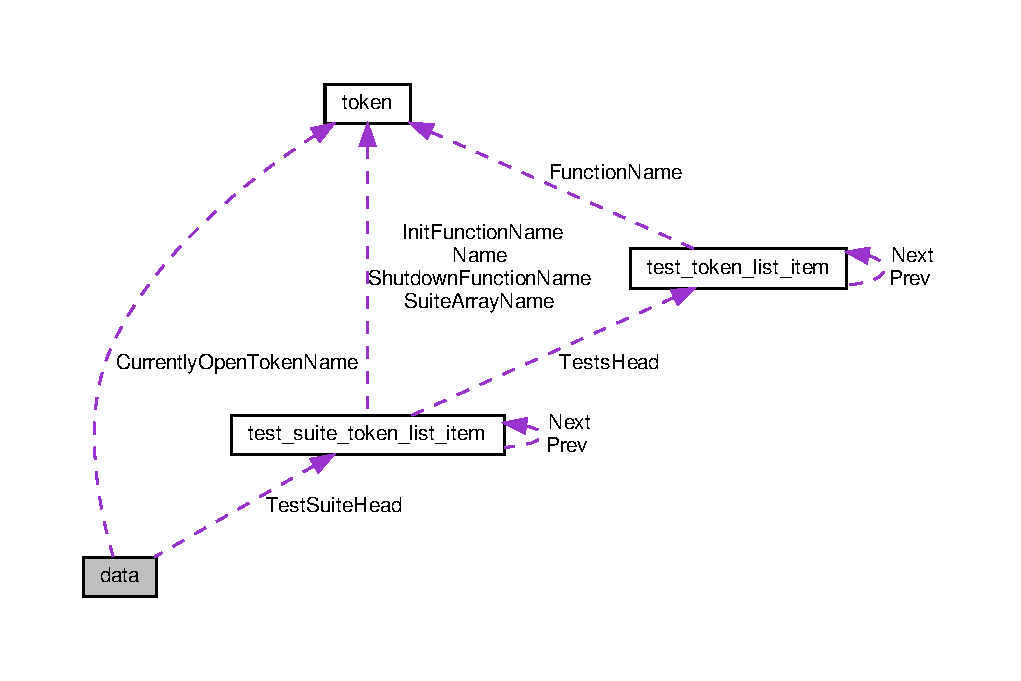
\includegraphics[width=350pt]{d7/dcf/structdata__coll__graph}
\end{center}
\end{figure}
\subsection*{Public Attributes}
\begin{DoxyCompactItemize}
\item 
memory\+\_\+arena \hyperlink{structdata_ad3188e5c8551b604c9d2c3ddbf29a9b8}{Memory}
\item 
\hyperlink{structtoken}{token} \hyperlink{structdata_acd39ca2feac118a8faa8d82520494213}{Currently\+Open\+Token\+Name}
\item 
\hyperlink{structtest__suite__token__list__item}{test\+\_\+suite\+\_\+token\+\_\+list\+\_\+item} \hyperlink{structdata_a5bb01b3754cb4b3baf9b7f499022cd1e}{Test\+Suite\+Head}
\end{DoxyCompactItemize}


\subsection{Member Data Documentation}
\mbox{\Hypertarget{structdata_acd39ca2feac118a8faa8d82520494213}\label{structdata_acd39ca2feac118a8faa8d82520494213}} 
\index{data@{data}!Currently\+Open\+Token\+Name@{Currently\+Open\+Token\+Name}}
\index{Currently\+Open\+Token\+Name@{Currently\+Open\+Token\+Name}!data@{data}}
\subsubsection{\texorpdfstring{Currently\+Open\+Token\+Name}{CurrentlyOpenTokenName}}
{\footnotesize\ttfamily \hyperlink{structtoken}{token} data\+::\+Currently\+Open\+Token\+Name}

\mbox{\Hypertarget{structdata_ad3188e5c8551b604c9d2c3ddbf29a9b8}\label{structdata_ad3188e5c8551b604c9d2c3ddbf29a9b8}} 
\index{data@{data}!Memory@{Memory}}
\index{Memory@{Memory}!data@{data}}
\subsubsection{\texorpdfstring{Memory}{Memory}}
{\footnotesize\ttfamily memory\+\_\+arena data\+::\+Memory}

\mbox{\Hypertarget{structdata_a5bb01b3754cb4b3baf9b7f499022cd1e}\label{structdata_a5bb01b3754cb4b3baf9b7f499022cd1e}} 
\index{data@{data}!Test\+Suite\+Head@{Test\+Suite\+Head}}
\index{Test\+Suite\+Head@{Test\+Suite\+Head}!data@{data}}
\subsubsection{\texorpdfstring{Test\+Suite\+Head}{TestSuiteHead}}
{\footnotesize\ttfamily \hyperlink{structtest__suite__token__list__item}{test\+\_\+suite\+\_\+token\+\_\+list\+\_\+item} data\+::\+Test\+Suite\+Head}



The documentation for this struct was generated from the following file\+:\begin{DoxyCompactItemize}
\item 
\hyperlink{test__preprocessor_8cpp}{test\+\_\+preprocessor.\+cpp}\end{DoxyCompactItemize}

\hypertarget{structlexer}{}\section{lexer Struct Reference}
\label{structlexer}\index{lexer@{lexer}}


{\ttfamily \#include $<$ab\+\_\+lexer.\+h$>$}

\subsection*{Public Attributes}
\begin{DoxyCompactItemize}
\item 
char $\ast$ \hyperlink{structlexer_a3a775702427156530a8b1c1f426a904d}{At}
\item 
\hyperlink{ab__common_8h_ae9b1af5c037e57a98884758875d3a7c4}{s32} \hyperlink{structlexer_a467733563699eba46da6c518ae3923eb}{Num\+Currently\+Open\+Braces}
\item 
\hyperlink{ab__common_8h_ae9b1af5c037e57a98884758875d3a7c4}{s32} \hyperlink{structlexer_a252d45a538fbf3a3b5a22c294061651c}{Line\+Number}
\end{DoxyCompactItemize}


\subsection{Member Data Documentation}
\mbox{\Hypertarget{structlexer_a3a775702427156530a8b1c1f426a904d}\label{structlexer_a3a775702427156530a8b1c1f426a904d}} 
\index{lexer@{lexer}!At@{At}}
\index{At@{At}!lexer@{lexer}}
\subsubsection{\texorpdfstring{At}{At}}
{\footnotesize\ttfamily char$\ast$ lexer\+::\+At}

\mbox{\Hypertarget{structlexer_a252d45a538fbf3a3b5a22c294061651c}\label{structlexer_a252d45a538fbf3a3b5a22c294061651c}} 
\index{lexer@{lexer}!Line\+Number@{Line\+Number}}
\index{Line\+Number@{Line\+Number}!lexer@{lexer}}
\subsubsection{\texorpdfstring{Line\+Number}{LineNumber}}
{\footnotesize\ttfamily \hyperlink{ab__common_8h_ae9b1af5c037e57a98884758875d3a7c4}{s32} lexer\+::\+Line\+Number}

\mbox{\Hypertarget{structlexer_a467733563699eba46da6c518ae3923eb}\label{structlexer_a467733563699eba46da6c518ae3923eb}} 
\index{lexer@{lexer}!Num\+Currently\+Open\+Braces@{Num\+Currently\+Open\+Braces}}
\index{Num\+Currently\+Open\+Braces@{Num\+Currently\+Open\+Braces}!lexer@{lexer}}
\subsubsection{\texorpdfstring{Num\+Currently\+Open\+Braces}{NumCurrentlyOpenBraces}}
{\footnotesize\ttfamily \hyperlink{ab__common_8h_ae9b1af5c037e57a98884758875d3a7c4}{s32} lexer\+::\+Num\+Currently\+Open\+Braces}



The documentation for this struct was generated from the following file\+:\begin{DoxyCompactItemize}
\item 
\hyperlink{ab__lexer_8h}{ab\+\_\+lexer.\+h}\end{DoxyCompactItemize}

\hypertarget{structmy__json__test}{}\doxysection{my\+\_\+json\+\_\+test Struct Reference}
\label{structmy__json__test}\index{my\_json\_test@{my\_json\_test}}


{\ttfamily \#include $<$Preproc\+Test.\+h$>$}

\doxysubsection*{Public Attributes}
\begin{DoxyCompactItemize}
\item 
u8 \mbox{\hyperlink{structmy__json__test_a0ea8af0c0061131955753275ad70dba4}{Test\+Unsigned}}
\item 
char \mbox{\hyperlink{structmy__json__test_a497da009ff7ce7742cf99571b0752227}{Test\+String}} \mbox{[}50\mbox{]}
\item 
\mbox{\hyperlink{PreprocTest_8h_a081cf1a0e70d6e2bd48c98f457742877}{en\+Colours}} \mbox{\hyperlink{structmy__json__test_a6f1212d5aaf1f688e8887d5614d510ca}{My\+Colour}}
\item 
b8 \mbox{\hyperlink{structmy__json__test_a55bffca96cce85232e33fc0c619a9eab}{is\+Value}}
\end{DoxyCompactItemize}


\doxysubsection{Member Data Documentation}
\mbox{\Hypertarget{structmy__json__test_a55bffca96cce85232e33fc0c619a9eab}\label{structmy__json__test_a55bffca96cce85232e33fc0c619a9eab}} 
\index{my\_json\_test@{my\_json\_test}!isValue@{isValue}}
\index{isValue@{isValue}!my\_json\_test@{my\_json\_test}}
\doxysubsubsection{\texorpdfstring{isValue}{isValue}}
{\footnotesize\ttfamily b8 my\+\_\+json\+\_\+test\+::is\+Value}

\mbox{\Hypertarget{structmy__json__test_a6f1212d5aaf1f688e8887d5614d510ca}\label{structmy__json__test_a6f1212d5aaf1f688e8887d5614d510ca}} 
\index{my\_json\_test@{my\_json\_test}!MyColour@{MyColour}}
\index{MyColour@{MyColour}!my\_json\_test@{my\_json\_test}}
\doxysubsubsection{\texorpdfstring{MyColour}{MyColour}}
{\footnotesize\ttfamily \mbox{\hyperlink{PreprocTest_8h_a081cf1a0e70d6e2bd48c98f457742877}{en\+Colours}} my\+\_\+json\+\_\+test\+::\+My\+Colour}

\mbox{\Hypertarget{structmy__json__test_a497da009ff7ce7742cf99571b0752227}\label{structmy__json__test_a497da009ff7ce7742cf99571b0752227}} 
\index{my\_json\_test@{my\_json\_test}!TestString@{TestString}}
\index{TestString@{TestString}!my\_json\_test@{my\_json\_test}}
\doxysubsubsection{\texorpdfstring{TestString}{TestString}}
{\footnotesize\ttfamily char my\+\_\+json\+\_\+test\+::\+Test\+String\mbox{[}50\mbox{]}}

\mbox{\Hypertarget{structmy__json__test_a0ea8af0c0061131955753275ad70dba4}\label{structmy__json__test_a0ea8af0c0061131955753275ad70dba4}} 
\index{my\_json\_test@{my\_json\_test}!TestUnsigned@{TestUnsigned}}
\index{TestUnsigned@{TestUnsigned}!my\_json\_test@{my\_json\_test}}
\doxysubsubsection{\texorpdfstring{TestUnsigned}{TestUnsigned}}
{\footnotesize\ttfamily u8 my\+\_\+json\+\_\+test\+::\+Test\+Unsigned}



The documentation for this struct was generated from the following file\+:\begin{DoxyCompactItemize}
\item 
\mbox{\hyperlink{PreprocTest_8h}{Preproc\+Test.\+h}}\end{DoxyCompactItemize}

\hypertarget{structmy__json__test__existlist}{}\section{my\+\_\+json\+\_\+test\+\_\+existlist Struct Reference}
\label{structmy__json__test__existlist}\index{my\+\_\+json\+\_\+test\+\_\+existlist@{my\+\_\+json\+\_\+test\+\_\+existlist}}


{\ttfamily \#include $<$Generated\+\_\+\+Test.\+h$>$}

\subsection*{Public Attributes}
\begin{DoxyCompactItemize}
\item 
\hyperlink{ab__common_8h_a70e369648385b50f2d0588e8e8745275}{b8} \hyperlink{structmy__json__test__existlist_abcc3320a088be44f3780f7768da67efa}{Test\+Unsigned}
\item 
\hyperlink{ab__common_8h_a70e369648385b50f2d0588e8e8745275}{b8} \hyperlink{structmy__json__test__existlist_ad1bf35a0d6153e177322567228ae0203}{Test\+String}
\item 
\hyperlink{ab__common_8h_a70e369648385b50f2d0588e8e8745275}{b8} \hyperlink{structmy__json__test__existlist_adc7bd401b4e560999733be88e43b5b7f}{My\+Colour}
\item 
\hyperlink{ab__common_8h_a70e369648385b50f2d0588e8e8745275}{b8} \hyperlink{structmy__json__test__existlist_ad8b82af159a6dd0709800ca082156caf}{is\+Value}
\end{DoxyCompactItemize}


\subsection{Member Data Documentation}
\mbox{\Hypertarget{structmy__json__test__existlist_ad8b82af159a6dd0709800ca082156caf}\label{structmy__json__test__existlist_ad8b82af159a6dd0709800ca082156caf}} 
\index{my\+\_\+json\+\_\+test\+\_\+existlist@{my\+\_\+json\+\_\+test\+\_\+existlist}!is\+Value@{is\+Value}}
\index{is\+Value@{is\+Value}!my\+\_\+json\+\_\+test\+\_\+existlist@{my\+\_\+json\+\_\+test\+\_\+existlist}}
\subsubsection{\texorpdfstring{is\+Value}{isValue}}
{\footnotesize\ttfamily \hyperlink{ab__common_8h_a70e369648385b50f2d0588e8e8745275}{b8} my\+\_\+json\+\_\+test\+\_\+existlist\+::is\+Value}

\mbox{\Hypertarget{structmy__json__test__existlist_adc7bd401b4e560999733be88e43b5b7f}\label{structmy__json__test__existlist_adc7bd401b4e560999733be88e43b5b7f}} 
\index{my\+\_\+json\+\_\+test\+\_\+existlist@{my\+\_\+json\+\_\+test\+\_\+existlist}!My\+Colour@{My\+Colour}}
\index{My\+Colour@{My\+Colour}!my\+\_\+json\+\_\+test\+\_\+existlist@{my\+\_\+json\+\_\+test\+\_\+existlist}}
\subsubsection{\texorpdfstring{My\+Colour}{MyColour}}
{\footnotesize\ttfamily \hyperlink{ab__common_8h_a70e369648385b50f2d0588e8e8745275}{b8} my\+\_\+json\+\_\+test\+\_\+existlist\+::\+My\+Colour}

\mbox{\Hypertarget{structmy__json__test__existlist_ad1bf35a0d6153e177322567228ae0203}\label{structmy__json__test__existlist_ad1bf35a0d6153e177322567228ae0203}} 
\index{my\+\_\+json\+\_\+test\+\_\+existlist@{my\+\_\+json\+\_\+test\+\_\+existlist}!Test\+String@{Test\+String}}
\index{Test\+String@{Test\+String}!my\+\_\+json\+\_\+test\+\_\+existlist@{my\+\_\+json\+\_\+test\+\_\+existlist}}
\subsubsection{\texorpdfstring{Test\+String}{TestString}}
{\footnotesize\ttfamily \hyperlink{ab__common_8h_a70e369648385b50f2d0588e8e8745275}{b8} my\+\_\+json\+\_\+test\+\_\+existlist\+::\+Test\+String}

\mbox{\Hypertarget{structmy__json__test__existlist_abcc3320a088be44f3780f7768da67efa}\label{structmy__json__test__existlist_abcc3320a088be44f3780f7768da67efa}} 
\index{my\+\_\+json\+\_\+test\+\_\+existlist@{my\+\_\+json\+\_\+test\+\_\+existlist}!Test\+Unsigned@{Test\+Unsigned}}
\index{Test\+Unsigned@{Test\+Unsigned}!my\+\_\+json\+\_\+test\+\_\+existlist@{my\+\_\+json\+\_\+test\+\_\+existlist}}
\subsubsection{\texorpdfstring{Test\+Unsigned}{TestUnsigned}}
{\footnotesize\ttfamily \hyperlink{ab__common_8h_a70e369648385b50f2d0588e8e8745275}{b8} my\+\_\+json\+\_\+test\+\_\+existlist\+::\+Test\+Unsigned}



The documentation for this struct was generated from the following file\+:\begin{DoxyCompactItemize}
\item 
\hyperlink{Generated__Test_8h}{Generated\+\_\+\+Test.\+h}\end{DoxyCompactItemize}

\hypertarget{structoutput__data}{}\section{output\+\_\+data Struct Reference}
\label{structoutput__data}\index{output\+\_\+data@{output\+\_\+data}}


{\ttfamily \#include $<$ab\+\_\+parser.\+h$>$}



Collaboration diagram for output\+\_\+data\+:\nopagebreak
\begin{figure}[H]
\begin{center}
\leavevmode
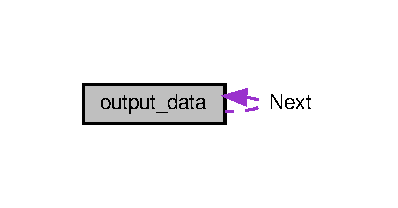
\includegraphics[width=191pt]{dc/d66/structoutput__data__coll__graph}
\end{center}
\end{figure}
\subsection*{Public Attributes}
\begin{DoxyCompactItemize}
\item 
char \hyperlink{structoutput__data_a4b5cddf8fc02cfb5219eafd71e3b3645}{Output\+String} \mbox{[}\hyperlink{ab__common_8h_a9e89c74d1fedd0a954107d7ab01481cc}{Kilobytes}(200)\mbox{]}
\item 
size\+\_\+t \hyperlink{structoutput__data_ac960304f0c5df1d42068abe8bb6a362a}{Used}
\item 
\hyperlink{structoutput__data}{output\+\_\+data} $\ast$ \hyperlink{structoutput__data_ab48e74baa16f37fe4f5b87faed472657}{Next}
\end{DoxyCompactItemize}


\subsection{Member Data Documentation}
\mbox{\Hypertarget{structoutput__data_ab48e74baa16f37fe4f5b87faed472657}\label{structoutput__data_ab48e74baa16f37fe4f5b87faed472657}} 
\index{output\+\_\+data@{output\+\_\+data}!Next@{Next}}
\index{Next@{Next}!output\+\_\+data@{output\+\_\+data}}
\subsubsection{\texorpdfstring{Next}{Next}}
{\footnotesize\ttfamily \hyperlink{structoutput__data}{output\+\_\+data}$\ast$ output\+\_\+data\+::\+Next}

\mbox{\Hypertarget{structoutput__data_a4b5cddf8fc02cfb5219eafd71e3b3645}\label{structoutput__data_a4b5cddf8fc02cfb5219eafd71e3b3645}} 
\index{output\+\_\+data@{output\+\_\+data}!Output\+String@{Output\+String}}
\index{Output\+String@{Output\+String}!output\+\_\+data@{output\+\_\+data}}
\subsubsection{\texorpdfstring{Output\+String}{OutputString}}
{\footnotesize\ttfamily char output\+\_\+data\+::\+Output\+String\mbox{[}\hyperlink{ab__common_8h_a9e89c74d1fedd0a954107d7ab01481cc}{Kilobytes}(200)\mbox{]}}

\mbox{\Hypertarget{structoutput__data_ac960304f0c5df1d42068abe8bb6a362a}\label{structoutput__data_ac960304f0c5df1d42068abe8bb6a362a}} 
\index{output\+\_\+data@{output\+\_\+data}!Used@{Used}}
\index{Used@{Used}!output\+\_\+data@{output\+\_\+data}}
\subsubsection{\texorpdfstring{Used}{Used}}
{\footnotesize\ttfamily size\+\_\+t output\+\_\+data\+::\+Used}



The documentation for this struct was generated from the following file\+:\begin{DoxyCompactItemize}
\item 
\hyperlink{ab__parser_8h}{ab\+\_\+parser.\+h}\end{DoxyCompactItemize}

\hypertarget{structparser}{}\section{parser Struct Reference}
\label{structparser}\index{parser@{parser}}


{\ttfamily \#include $<$ab\+\_\+parser.\+h$>$}



Collaboration diagram for parser\+:\nopagebreak
\begin{figure}[H]
\begin{center}
\leavevmode
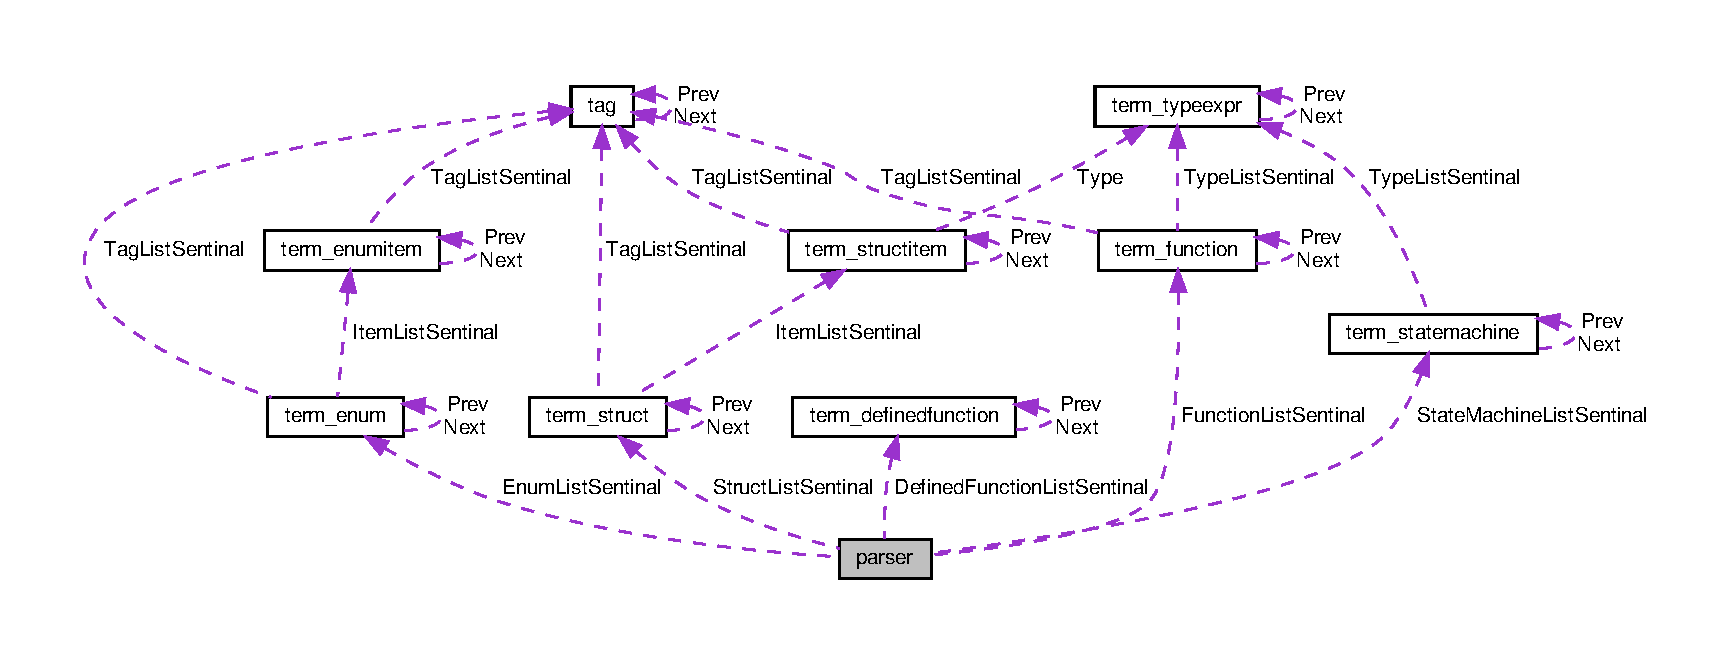
\includegraphics[width=350pt]{d1/d68/structparser__coll__graph}
\end{center}
\end{figure}
\subsection*{Public Attributes}
\begin{DoxyCompactItemize}
\item 
\hyperlink{structmemory__arena}{memory\+\_\+arena} $\ast$ \hyperlink{structparser_ae92434364d983495b64df17550f40d27}{Memory}
\item 
\hyperlink{structterm__struct}{term\+\_\+struct} \hyperlink{structparser_accfacf760af582468d591a06259406be}{Struct\+List\+Sentinal}
\item 
\hyperlink{structterm__enum}{term\+\_\+enum} \hyperlink{structparser_a8023ac3e70ded1ba71e6a2974a9e22b6}{Enum\+List\+Sentinal}
\item 
\hyperlink{structterm__function}{term\+\_\+function} \hyperlink{structparser_a43e51e28e997b7acf6121eb6e6a894f1}{Function\+List\+Sentinal}
\item 
\hyperlink{structterm__statemachine}{term\+\_\+statemachine} \hyperlink{structparser_aa29d6dda9d3d933604823ec27584f162}{State\+Machine\+List\+Sentinal}
\item 
\hyperlink{structterm__definedfunction}{term\+\_\+definedfunction} \hyperlink{structparser_a536dbd6d3a451a05b2365772bd5533a5}{Defined\+Function\+List\+Sentinal}
\end{DoxyCompactItemize}


\subsection{Member Data Documentation}
\mbox{\Hypertarget{structparser_a536dbd6d3a451a05b2365772bd5533a5}\label{structparser_a536dbd6d3a451a05b2365772bd5533a5}} 
\index{parser@{parser}!Defined\+Function\+List\+Sentinal@{Defined\+Function\+List\+Sentinal}}
\index{Defined\+Function\+List\+Sentinal@{Defined\+Function\+List\+Sentinal}!parser@{parser}}
\subsubsection{\texorpdfstring{Defined\+Function\+List\+Sentinal}{DefinedFunctionListSentinal}}
{\footnotesize\ttfamily \hyperlink{structterm__definedfunction}{term\+\_\+definedfunction} parser\+::\+Defined\+Function\+List\+Sentinal}

\mbox{\Hypertarget{structparser_a8023ac3e70ded1ba71e6a2974a9e22b6}\label{structparser_a8023ac3e70ded1ba71e6a2974a9e22b6}} 
\index{parser@{parser}!Enum\+List\+Sentinal@{Enum\+List\+Sentinal}}
\index{Enum\+List\+Sentinal@{Enum\+List\+Sentinal}!parser@{parser}}
\subsubsection{\texorpdfstring{Enum\+List\+Sentinal}{EnumListSentinal}}
{\footnotesize\ttfamily \hyperlink{structterm__enum}{term\+\_\+enum} parser\+::\+Enum\+List\+Sentinal}

\mbox{\Hypertarget{structparser_a43e51e28e997b7acf6121eb6e6a894f1}\label{structparser_a43e51e28e997b7acf6121eb6e6a894f1}} 
\index{parser@{parser}!Function\+List\+Sentinal@{Function\+List\+Sentinal}}
\index{Function\+List\+Sentinal@{Function\+List\+Sentinal}!parser@{parser}}
\subsubsection{\texorpdfstring{Function\+List\+Sentinal}{FunctionListSentinal}}
{\footnotesize\ttfamily \hyperlink{structterm__function}{term\+\_\+function} parser\+::\+Function\+List\+Sentinal}

\mbox{\Hypertarget{structparser_ae92434364d983495b64df17550f40d27}\label{structparser_ae92434364d983495b64df17550f40d27}} 
\index{parser@{parser}!Memory@{Memory}}
\index{Memory@{Memory}!parser@{parser}}
\subsubsection{\texorpdfstring{Memory}{Memory}}
{\footnotesize\ttfamily \hyperlink{structmemory__arena}{memory\+\_\+arena}$\ast$ parser\+::\+Memory}

\mbox{\Hypertarget{structparser_aa29d6dda9d3d933604823ec27584f162}\label{structparser_aa29d6dda9d3d933604823ec27584f162}} 
\index{parser@{parser}!State\+Machine\+List\+Sentinal@{State\+Machine\+List\+Sentinal}}
\index{State\+Machine\+List\+Sentinal@{State\+Machine\+List\+Sentinal}!parser@{parser}}
\subsubsection{\texorpdfstring{State\+Machine\+List\+Sentinal}{StateMachineListSentinal}}
{\footnotesize\ttfamily \hyperlink{structterm__statemachine}{term\+\_\+statemachine} parser\+::\+State\+Machine\+List\+Sentinal}

\mbox{\Hypertarget{structparser_accfacf760af582468d591a06259406be}\label{structparser_accfacf760af582468d591a06259406be}} 
\index{parser@{parser}!Struct\+List\+Sentinal@{Struct\+List\+Sentinal}}
\index{Struct\+List\+Sentinal@{Struct\+List\+Sentinal}!parser@{parser}}
\subsubsection{\texorpdfstring{Struct\+List\+Sentinal}{StructListSentinal}}
{\footnotesize\ttfamily \hyperlink{structterm__struct}{term\+\_\+struct} parser\+::\+Struct\+List\+Sentinal}



The documentation for this struct was generated from the following file\+:\begin{DoxyCompactItemize}
\item 
\hyperlink{ab__parser_8h}{ab\+\_\+parser.\+h}\end{DoxyCompactItemize}

\hypertarget{structtag}{}\section{tag Struct Reference}
\label{structtag}\index{tag@{tag}}


{\ttfamily \#include $<$ab\+\_\+parser.\+h$>$}



Collaboration diagram for tag\+:\nopagebreak
\begin{figure}[H]
\begin{center}
\leavevmode
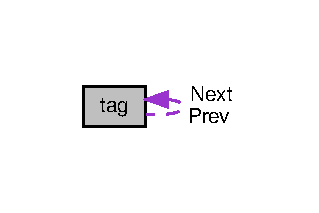
\includegraphics[width=174pt]{db/d25/structtag__coll__graph}
\end{center}
\end{figure}
\subsection*{Public Attributes}
\begin{DoxyCompactItemize}
\item 
\hyperlink{structabs__stringptr}{abs\+\_\+stringptr} \hyperlink{structtag_a4564f437775d5276bcddbc23a6b8881e}{Name}
\item 
\hyperlink{structabs__stringptr}{abs\+\_\+stringptr} \hyperlink{structtag_aa52b4f28c97f8ff006a5fe50d6623a7e}{Option}
\item 
\hyperlink{structtag}{tag} $\ast$ \hyperlink{structtag_ae16f0e5fb461cdbae551134f3e1e8e24}{Next}
\item 
\hyperlink{structtag}{tag} $\ast$ \hyperlink{structtag_af05983b55100a16b3bcd8faad9b50e00}{Prev}
\end{DoxyCompactItemize}


\subsection{Member Data Documentation}
\mbox{\Hypertarget{structtag_a4564f437775d5276bcddbc23a6b8881e}\label{structtag_a4564f437775d5276bcddbc23a6b8881e}} 
\index{tag@{tag}!Name@{Name}}
\index{Name@{Name}!tag@{tag}}
\subsubsection{\texorpdfstring{Name}{Name}}
{\footnotesize\ttfamily \hyperlink{structabs__stringptr}{abs\+\_\+stringptr} tag\+::\+Name}

\mbox{\Hypertarget{structtag_ae16f0e5fb461cdbae551134f3e1e8e24}\label{structtag_ae16f0e5fb461cdbae551134f3e1e8e24}} 
\index{tag@{tag}!Next@{Next}}
\index{Next@{Next}!tag@{tag}}
\subsubsection{\texorpdfstring{Next}{Next}}
{\footnotesize\ttfamily \hyperlink{structtag}{tag}$\ast$ tag\+::\+Next}

\mbox{\Hypertarget{structtag_aa52b4f28c97f8ff006a5fe50d6623a7e}\label{structtag_aa52b4f28c97f8ff006a5fe50d6623a7e}} 
\index{tag@{tag}!Option@{Option}}
\index{Option@{Option}!tag@{tag}}
\subsubsection{\texorpdfstring{Option}{Option}}
{\footnotesize\ttfamily \hyperlink{structabs__stringptr}{abs\+\_\+stringptr} tag\+::\+Option}

\mbox{\Hypertarget{structtag_af05983b55100a16b3bcd8faad9b50e00}\label{structtag_af05983b55100a16b3bcd8faad9b50e00}} 
\index{tag@{tag}!Prev@{Prev}}
\index{Prev@{Prev}!tag@{tag}}
\subsubsection{\texorpdfstring{Prev}{Prev}}
{\footnotesize\ttfamily \hyperlink{structtag}{tag}$\ast$ tag\+::\+Prev}



The documentation for this struct was generated from the following file\+:\begin{DoxyCompactItemize}
\item 
\hyperlink{ab__parser_8h}{ab\+\_\+parser.\+h}\end{DoxyCompactItemize}

\hypertarget{structterm__definedfunction}{}\doxysection{term\+\_\+definedfunction Struct Reference}
\label{structterm__definedfunction}\index{term\_definedfunction@{term\_definedfunction}}


{\ttfamily \#include $<$ab\+\_\+parser.\+h$>$}



Collaboration diagram for term\+\_\+definedfunction\+:\nopagebreak
\begin{figure}[H]
\begin{center}
\leavevmode
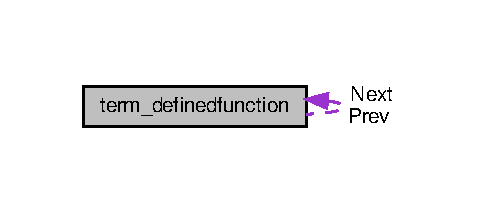
\includegraphics[width=230pt]{df/da2/structterm__definedfunction__coll__graph}
\end{center}
\end{figure}
\doxysubsection*{Public Attributes}
\begin{DoxyCompactItemize}
\item 
st\+\_\+ptr \mbox{\hyperlink{structterm__definedfunction_ad55b79d386e27412ffe321d1543c5a97}{Define}}
\item 
st\+\_\+ptr \mbox{\hyperlink{structterm__definedfunction_a0ca3f3ba52e981e2be9549ea533f7d60}{Name}}
\item 
\mbox{\hyperlink{structterm__definedfunction}{term\+\_\+definedfunction}} $\ast$ \mbox{\hyperlink{structterm__definedfunction_ae4d62f23998fa05c8b5e4e900980460c}{Next}}
\item 
\mbox{\hyperlink{structterm__definedfunction}{term\+\_\+definedfunction}} $\ast$ \mbox{\hyperlink{structterm__definedfunction_a8f3ed1e8ae1fa3012452929ca8cb0da3}{Prev}}
\end{DoxyCompactItemize}


\doxysubsection{Member Data Documentation}
\mbox{\Hypertarget{structterm__definedfunction_ad55b79d386e27412ffe321d1543c5a97}\label{structterm__definedfunction_ad55b79d386e27412ffe321d1543c5a97}} 
\index{term\_definedfunction@{term\_definedfunction}!Define@{Define}}
\index{Define@{Define}!term\_definedfunction@{term\_definedfunction}}
\doxysubsubsection{\texorpdfstring{Define}{Define}}
{\footnotesize\ttfamily st\+\_\+ptr term\+\_\+definedfunction\+::\+Define}

\mbox{\Hypertarget{structterm__definedfunction_a0ca3f3ba52e981e2be9549ea533f7d60}\label{structterm__definedfunction_a0ca3f3ba52e981e2be9549ea533f7d60}} 
\index{term\_definedfunction@{term\_definedfunction}!Name@{Name}}
\index{Name@{Name}!term\_definedfunction@{term\_definedfunction}}
\doxysubsubsection{\texorpdfstring{Name}{Name}}
{\footnotesize\ttfamily st\+\_\+ptr term\+\_\+definedfunction\+::\+Name}

\mbox{\Hypertarget{structterm__definedfunction_ae4d62f23998fa05c8b5e4e900980460c}\label{structterm__definedfunction_ae4d62f23998fa05c8b5e4e900980460c}} 
\index{term\_definedfunction@{term\_definedfunction}!Next@{Next}}
\index{Next@{Next}!term\_definedfunction@{term\_definedfunction}}
\doxysubsubsection{\texorpdfstring{Next}{Next}}
{\footnotesize\ttfamily \mbox{\hyperlink{structterm__definedfunction}{term\+\_\+definedfunction}}$\ast$ term\+\_\+definedfunction\+::\+Next}

\mbox{\Hypertarget{structterm__definedfunction_a8f3ed1e8ae1fa3012452929ca8cb0da3}\label{structterm__definedfunction_a8f3ed1e8ae1fa3012452929ca8cb0da3}} 
\index{term\_definedfunction@{term\_definedfunction}!Prev@{Prev}}
\index{Prev@{Prev}!term\_definedfunction@{term\_definedfunction}}
\doxysubsubsection{\texorpdfstring{Prev}{Prev}}
{\footnotesize\ttfamily \mbox{\hyperlink{structterm__definedfunction}{term\+\_\+definedfunction}}$\ast$ term\+\_\+definedfunction\+::\+Prev}



The documentation for this struct was generated from the following file\+:\begin{DoxyCompactItemize}
\item 
\mbox{\hyperlink{ab__parser_8h}{ab\+\_\+parser.\+h}}\end{DoxyCompactItemize}

\hypertarget{structterm__enum}{}\section{term\+\_\+enum Struct Reference}
\label{structterm__enum}\index{term\+\_\+enum@{term\+\_\+enum}}


{\ttfamily \#include $<$ab\+\_\+parser.\+h$>$}



Collaboration diagram for term\+\_\+enum\+:\nopagebreak
\begin{figure}[H]
\begin{center}
\leavevmode
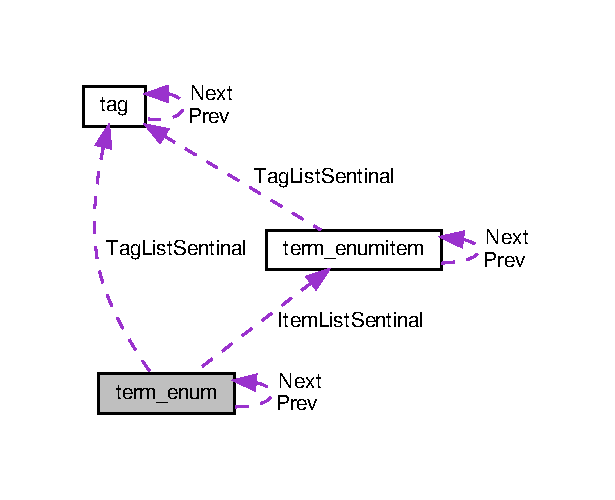
\includegraphics[width=309pt]{d6/d82/structterm__enum__coll__graph}
\end{center}
\end{figure}
\subsection*{Public Attributes}
\begin{DoxyCompactItemize}
\item 
\hyperlink{structabs__stringptr}{abs\+\_\+stringptr} \hyperlink{structterm__enum_a41929255cd1231f08655f7440bd2051f}{Name}
\item 
\hyperlink{structtag}{tag} \hyperlink{structterm__enum_a064766a8666ff84a4571dff4d9a7070a}{Tag\+List\+Sentinal}
\item 
\hyperlink{structterm__enumitem}{term\+\_\+enumitem} \hyperlink{structterm__enum_a982f44fe4692493e3456a80b50805d64}{Item\+List\+Sentinal}
\item 
\hyperlink{ab__common_8h_afaa62991928fb9fb18ff0db62a040aba}{u32} \hyperlink{structterm__enum_a90cb3e473c1ca0a59037e3882af7a1bc}{Item\+Count}
\item 
\hyperlink{structterm__enum}{term\+\_\+enum} $\ast$ \hyperlink{structterm__enum_aa66270184b4f4d6457dda0afd18e25fc}{Next}
\item 
\hyperlink{structterm__enum}{term\+\_\+enum} $\ast$ \hyperlink{structterm__enum_addad4748b3a035a56ed83b5389668f35}{Prev}
\end{DoxyCompactItemize}


\subsection{Member Data Documentation}
\mbox{\Hypertarget{structterm__enum_a90cb3e473c1ca0a59037e3882af7a1bc}\label{structterm__enum_a90cb3e473c1ca0a59037e3882af7a1bc}} 
\index{term\+\_\+enum@{term\+\_\+enum}!Item\+Count@{Item\+Count}}
\index{Item\+Count@{Item\+Count}!term\+\_\+enum@{term\+\_\+enum}}
\subsubsection{\texorpdfstring{Item\+Count}{ItemCount}}
{\footnotesize\ttfamily \hyperlink{ab__common_8h_afaa62991928fb9fb18ff0db62a040aba}{u32} term\+\_\+enum\+::\+Item\+Count}

\mbox{\Hypertarget{structterm__enum_a982f44fe4692493e3456a80b50805d64}\label{structterm__enum_a982f44fe4692493e3456a80b50805d64}} 
\index{term\+\_\+enum@{term\+\_\+enum}!Item\+List\+Sentinal@{Item\+List\+Sentinal}}
\index{Item\+List\+Sentinal@{Item\+List\+Sentinal}!term\+\_\+enum@{term\+\_\+enum}}
\subsubsection{\texorpdfstring{Item\+List\+Sentinal}{ItemListSentinal}}
{\footnotesize\ttfamily \hyperlink{structterm__enumitem}{term\+\_\+enumitem} term\+\_\+enum\+::\+Item\+List\+Sentinal}

\mbox{\Hypertarget{structterm__enum_a41929255cd1231f08655f7440bd2051f}\label{structterm__enum_a41929255cd1231f08655f7440bd2051f}} 
\index{term\+\_\+enum@{term\+\_\+enum}!Name@{Name}}
\index{Name@{Name}!term\+\_\+enum@{term\+\_\+enum}}
\subsubsection{\texorpdfstring{Name}{Name}}
{\footnotesize\ttfamily \hyperlink{structabs__stringptr}{abs\+\_\+stringptr} term\+\_\+enum\+::\+Name}

\mbox{\Hypertarget{structterm__enum_aa66270184b4f4d6457dda0afd18e25fc}\label{structterm__enum_aa66270184b4f4d6457dda0afd18e25fc}} 
\index{term\+\_\+enum@{term\+\_\+enum}!Next@{Next}}
\index{Next@{Next}!term\+\_\+enum@{term\+\_\+enum}}
\subsubsection{\texorpdfstring{Next}{Next}}
{\footnotesize\ttfamily \hyperlink{structterm__enum}{term\+\_\+enum}$\ast$ term\+\_\+enum\+::\+Next}

\mbox{\Hypertarget{structterm__enum_addad4748b3a035a56ed83b5389668f35}\label{structterm__enum_addad4748b3a035a56ed83b5389668f35}} 
\index{term\+\_\+enum@{term\+\_\+enum}!Prev@{Prev}}
\index{Prev@{Prev}!term\+\_\+enum@{term\+\_\+enum}}
\subsubsection{\texorpdfstring{Prev}{Prev}}
{\footnotesize\ttfamily \hyperlink{structterm__enum}{term\+\_\+enum}$\ast$ term\+\_\+enum\+::\+Prev}

\mbox{\Hypertarget{structterm__enum_a064766a8666ff84a4571dff4d9a7070a}\label{structterm__enum_a064766a8666ff84a4571dff4d9a7070a}} 
\index{term\+\_\+enum@{term\+\_\+enum}!Tag\+List\+Sentinal@{Tag\+List\+Sentinal}}
\index{Tag\+List\+Sentinal@{Tag\+List\+Sentinal}!term\+\_\+enum@{term\+\_\+enum}}
\subsubsection{\texorpdfstring{Tag\+List\+Sentinal}{TagListSentinal}}
{\footnotesize\ttfamily \hyperlink{structtag}{tag} term\+\_\+enum\+::\+Tag\+List\+Sentinal}



The documentation for this struct was generated from the following file\+:\begin{DoxyCompactItemize}
\item 
\hyperlink{ab__parser_8h}{ab\+\_\+parser.\+h}\end{DoxyCompactItemize}

\hypertarget{structterm__enumitem}{}\doxysection{term\+\_\+enumitem Struct Reference}
\label{structterm__enumitem}\index{term\_enumitem@{term\_enumitem}}


{\ttfamily \#include $<$ab\+\_\+parser.\+h$>$}



Collaboration diagram for term\+\_\+enumitem\+:\nopagebreak
\begin{figure}[H]
\begin{center}
\leavevmode
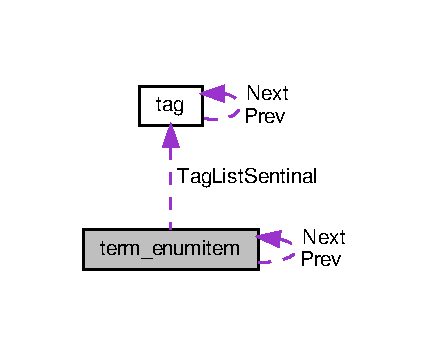
\includegraphics[width=207pt]{dc/def/structterm__enumitem__coll__graph}
\end{center}
\end{figure}
\doxysubsection*{Public Attributes}
\begin{DoxyCompactItemize}
\item 
st\+\_\+ptr \mbox{\hyperlink{structterm__enumitem_a5786103cf50b4967f5901683bfa19625}{Name}}
\item 
\mbox{\hyperlink{structtag}{tag}} \mbox{\hyperlink{structterm__enumitem_ace61cab8da4a090548e03c7a9970deb1}{Tag\+List\+Sentinal}}
\item 
\mbox{\hyperlink{structterm__enumitem}{term\+\_\+enumitem}} $\ast$ \mbox{\hyperlink{structterm__enumitem_a76a5df14c05395f4737800d06c23611a}{Next}}
\item 
\mbox{\hyperlink{structterm__enumitem}{term\+\_\+enumitem}} $\ast$ \mbox{\hyperlink{structterm__enumitem_a9841d521b128ff1d85936bdfded2e425}{Prev}}
\end{DoxyCompactItemize}


\doxysubsection{Member Data Documentation}
\mbox{\Hypertarget{structterm__enumitem_a5786103cf50b4967f5901683bfa19625}\label{structterm__enumitem_a5786103cf50b4967f5901683bfa19625}} 
\index{term\_enumitem@{term\_enumitem}!Name@{Name}}
\index{Name@{Name}!term\_enumitem@{term\_enumitem}}
\doxysubsubsection{\texorpdfstring{Name}{Name}}
{\footnotesize\ttfamily st\+\_\+ptr term\+\_\+enumitem\+::\+Name}

\mbox{\Hypertarget{structterm__enumitem_a76a5df14c05395f4737800d06c23611a}\label{structterm__enumitem_a76a5df14c05395f4737800d06c23611a}} 
\index{term\_enumitem@{term\_enumitem}!Next@{Next}}
\index{Next@{Next}!term\_enumitem@{term\_enumitem}}
\doxysubsubsection{\texorpdfstring{Next}{Next}}
{\footnotesize\ttfamily \mbox{\hyperlink{structterm__enumitem}{term\+\_\+enumitem}}$\ast$ term\+\_\+enumitem\+::\+Next}

\mbox{\Hypertarget{structterm__enumitem_a9841d521b128ff1d85936bdfded2e425}\label{structterm__enumitem_a9841d521b128ff1d85936bdfded2e425}} 
\index{term\_enumitem@{term\_enumitem}!Prev@{Prev}}
\index{Prev@{Prev}!term\_enumitem@{term\_enumitem}}
\doxysubsubsection{\texorpdfstring{Prev}{Prev}}
{\footnotesize\ttfamily \mbox{\hyperlink{structterm__enumitem}{term\+\_\+enumitem}}$\ast$ term\+\_\+enumitem\+::\+Prev}

\mbox{\Hypertarget{structterm__enumitem_ace61cab8da4a090548e03c7a9970deb1}\label{structterm__enumitem_ace61cab8da4a090548e03c7a9970deb1}} 
\index{term\_enumitem@{term\_enumitem}!TagListSentinal@{TagListSentinal}}
\index{TagListSentinal@{TagListSentinal}!term\_enumitem@{term\_enumitem}}
\doxysubsubsection{\texorpdfstring{TagListSentinal}{TagListSentinal}}
{\footnotesize\ttfamily \mbox{\hyperlink{structtag}{tag}} term\+\_\+enumitem\+::\+Tag\+List\+Sentinal}



The documentation for this struct was generated from the following file\+:\begin{DoxyCompactItemize}
\item 
\mbox{\hyperlink{ab__parser_8h}{ab\+\_\+parser.\+h}}\end{DoxyCompactItemize}

\hypertarget{structterm__function}{}\section{term\+\_\+function Struct Reference}
\label{structterm__function}\index{term\+\_\+function@{term\+\_\+function}}


{\ttfamily \#include $<$ab\+\_\+parser.\+h$>$}



Collaboration diagram for term\+\_\+function\+:
\nopagebreak
\begin{figure}[H]
\begin{center}
\leavevmode
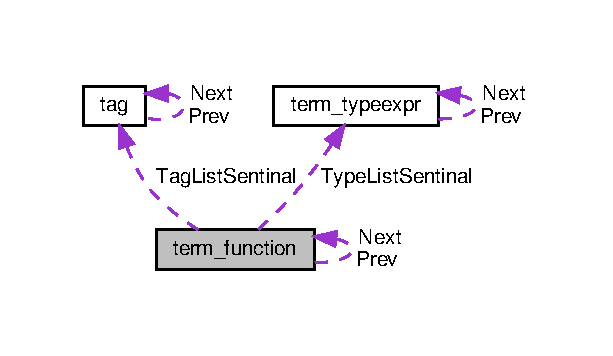
\includegraphics[width=292pt]{d0/dd8/structterm__function__coll__graph}
\end{center}
\end{figure}
\subsection*{Public Attributes}
\begin{DoxyCompactItemize}
\item 
abs\+\_\+stringptr \hyperlink{structterm__function_a44d4f15308d31174ac9443aeefe9544a}{Name}
\item 
\hyperlink{structtag}{tag} \hyperlink{structterm__function_ab3a3bd4264776e6fe2d04b161bd62433}{Tag\+List\+Sentinal}
\item 
\hyperlink{structterm__typeexpr}{term\+\_\+typeexpr} \hyperlink{structterm__function_a96b877553f990184a9da245207de9524}{Type\+List\+Sentinal}
\item 
u32 \hyperlink{structterm__function_a4e47cbfb96047c0ed4e06e87e079fb6a}{Type\+Count}
\item 
\hyperlink{structterm__function}{term\+\_\+function} $\ast$ \hyperlink{structterm__function_a655992a45b7bc18c8208d9a058bb86e6}{Next}
\item 
\hyperlink{structterm__function}{term\+\_\+function} $\ast$ \hyperlink{structterm__function_aab58e6419571c457d2b7563724bed629}{Prev}
\end{DoxyCompactItemize}


\subsection{Member Data Documentation}
\mbox{\Hypertarget{structterm__function_a44d4f15308d31174ac9443aeefe9544a}\label{structterm__function_a44d4f15308d31174ac9443aeefe9544a}} 
\index{term\+\_\+function@{term\+\_\+function}!Name@{Name}}
\index{Name@{Name}!term\+\_\+function@{term\+\_\+function}}
\subsubsection{\texorpdfstring{Name}{Name}}
{\footnotesize\ttfamily abs\+\_\+stringptr term\+\_\+function\+::\+Name}

\mbox{\Hypertarget{structterm__function_a655992a45b7bc18c8208d9a058bb86e6}\label{structterm__function_a655992a45b7bc18c8208d9a058bb86e6}} 
\index{term\+\_\+function@{term\+\_\+function}!Next@{Next}}
\index{Next@{Next}!term\+\_\+function@{term\+\_\+function}}
\subsubsection{\texorpdfstring{Next}{Next}}
{\footnotesize\ttfamily \hyperlink{structterm__function}{term\+\_\+function}$\ast$ term\+\_\+function\+::\+Next}

\mbox{\Hypertarget{structterm__function_aab58e6419571c457d2b7563724bed629}\label{structterm__function_aab58e6419571c457d2b7563724bed629}} 
\index{term\+\_\+function@{term\+\_\+function}!Prev@{Prev}}
\index{Prev@{Prev}!term\+\_\+function@{term\+\_\+function}}
\subsubsection{\texorpdfstring{Prev}{Prev}}
{\footnotesize\ttfamily \hyperlink{structterm__function}{term\+\_\+function}$\ast$ term\+\_\+function\+::\+Prev}

\mbox{\Hypertarget{structterm__function_ab3a3bd4264776e6fe2d04b161bd62433}\label{structterm__function_ab3a3bd4264776e6fe2d04b161bd62433}} 
\index{term\+\_\+function@{term\+\_\+function}!Tag\+List\+Sentinal@{Tag\+List\+Sentinal}}
\index{Tag\+List\+Sentinal@{Tag\+List\+Sentinal}!term\+\_\+function@{term\+\_\+function}}
\subsubsection{\texorpdfstring{Tag\+List\+Sentinal}{TagListSentinal}}
{\footnotesize\ttfamily \hyperlink{structtag}{tag} term\+\_\+function\+::\+Tag\+List\+Sentinal}

\mbox{\Hypertarget{structterm__function_a4e47cbfb96047c0ed4e06e87e079fb6a}\label{structterm__function_a4e47cbfb96047c0ed4e06e87e079fb6a}} 
\index{term\+\_\+function@{term\+\_\+function}!Type\+Count@{Type\+Count}}
\index{Type\+Count@{Type\+Count}!term\+\_\+function@{term\+\_\+function}}
\subsubsection{\texorpdfstring{Type\+Count}{TypeCount}}
{\footnotesize\ttfamily u32 term\+\_\+function\+::\+Type\+Count}

\mbox{\Hypertarget{structterm__function_a96b877553f990184a9da245207de9524}\label{structterm__function_a96b877553f990184a9da245207de9524}} 
\index{term\+\_\+function@{term\+\_\+function}!Type\+List\+Sentinal@{Type\+List\+Sentinal}}
\index{Type\+List\+Sentinal@{Type\+List\+Sentinal}!term\+\_\+function@{term\+\_\+function}}
\subsubsection{\texorpdfstring{Type\+List\+Sentinal}{TypeListSentinal}}
{\footnotesize\ttfamily \hyperlink{structterm__typeexpr}{term\+\_\+typeexpr} term\+\_\+function\+::\+Type\+List\+Sentinal}



The documentation for this struct was generated from the following file\+:\begin{DoxyCompactItemize}
\item 
\hyperlink{ab__parser_8h}{ab\+\_\+parser.\+h}\end{DoxyCompactItemize}

\hypertarget{structterm__statefunction}{}\doxysection{term\+\_\+statefunction Struct Reference}
\label{structterm__statefunction}\index{term\_statefunction@{term\_statefunction}}


{\ttfamily \#include $<$ab\+\_\+parser.\+h$>$}



Collaboration diagram for term\+\_\+statefunction\+:
\nopagebreak
\begin{figure}[H]
\begin{center}
\leavevmode
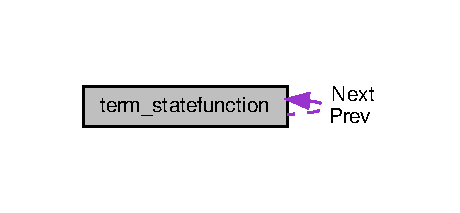
\includegraphics[width=221pt]{dd/d3e/structterm__statefunction__coll__graph}
\end{center}
\end{figure}
\doxysubsection*{Public Attributes}
\begin{DoxyCompactItemize}
\item 
\mbox{\hyperlink{structterm__statefunction}{term\+\_\+statefunction}} $\ast$ \mbox{\hyperlink{structterm__statefunction_a326dae1852433ae2fc11195dd1770ddf}{Next}}
\item 
\mbox{\hyperlink{structterm__statefunction}{term\+\_\+statefunction}} $\ast$ \mbox{\hyperlink{structterm__statefunction_a2693cbcd59a8a1eea7cbc1f8a61efc83}{Prev}}
\end{DoxyCompactItemize}


\doxysubsection{Member Data Documentation}
\mbox{\Hypertarget{structterm__statefunction_a326dae1852433ae2fc11195dd1770ddf}\label{structterm__statefunction_a326dae1852433ae2fc11195dd1770ddf}} 
\index{term\_statefunction@{term\_statefunction}!Next@{Next}}
\index{Next@{Next}!term\_statefunction@{term\_statefunction}}
\doxysubsubsection{\texorpdfstring{Next}{Next}}
{\footnotesize\ttfamily \mbox{\hyperlink{structterm__statefunction}{term\+\_\+statefunction}}$\ast$ term\+\_\+statefunction\+::\+Next}

\mbox{\Hypertarget{structterm__statefunction_a2693cbcd59a8a1eea7cbc1f8a61efc83}\label{structterm__statefunction_a2693cbcd59a8a1eea7cbc1f8a61efc83}} 
\index{term\_statefunction@{term\_statefunction}!Prev@{Prev}}
\index{Prev@{Prev}!term\_statefunction@{term\_statefunction}}
\doxysubsubsection{\texorpdfstring{Prev}{Prev}}
{\footnotesize\ttfamily \mbox{\hyperlink{structterm__statefunction}{term\+\_\+statefunction}}$\ast$ term\+\_\+statefunction\+::\+Prev}



The documentation for this struct was generated from the following file\+:\begin{DoxyCompactItemize}
\item 
\mbox{\hyperlink{ab__parser_8h}{ab\+\_\+parser.\+h}}\end{DoxyCompactItemize}

\hypertarget{structterm__statemachine}{}\doxysection{term\+\_\+statemachine Struct Reference}
\label{structterm__statemachine}\index{term\_statemachine@{term\_statemachine}}


{\ttfamily \#include $<$ab\+\_\+parser.\+h$>$}



Collaboration diagram for term\+\_\+statemachine\+:\nopagebreak
\begin{figure}[H]
\begin{center}
\leavevmode
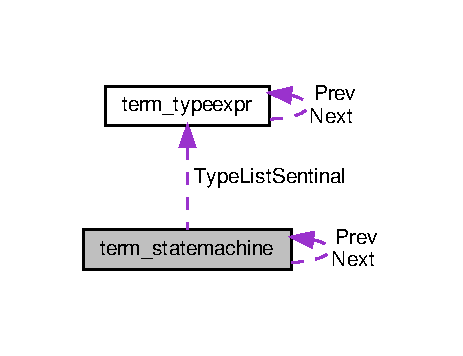
\includegraphics[width=223pt]{de/d7c/structterm__statemachine__coll__graph}
\end{center}
\end{figure}
\doxysubsection*{Public Attributes}
\begin{DoxyCompactItemize}
\item 
st\+\_\+ptr \mbox{\hyperlink{structterm__statemachine_a4c8a27598b9cd9eb13f905ff963ffe24}{Function}}
\item 
st\+\_\+ptr \mbox{\hyperlink{structterm__statemachine_a11af23252a3c9c1a3d7959e905800bae}{Type}}
\item 
st\+\_\+ptr \mbox{\hyperlink{structterm__statemachine_a2f1fc1d8b4b0a816f7ddfe8105a1ce54}{Cmd}}
\item 
\mbox{\hyperlink{structterm__typeexpr}{term\+\_\+typeexpr}} \mbox{\hyperlink{structterm__statemachine_ababd4f7bc69e5ca15fe95a56cdb312af}{Type\+List\+Sentinal}}
\item 
\mbox{\hyperlink{structterm__statemachine}{term\+\_\+statemachine}} $\ast$ \mbox{\hyperlink{structterm__statemachine_a78279e94d1a4f84463c5d7c4fba6bc17}{Next}}
\item 
\mbox{\hyperlink{structterm__statemachine}{term\+\_\+statemachine}} $\ast$ \mbox{\hyperlink{structterm__statemachine_a4e1ec651310e6e0789f9bcb627cfaa70}{Prev}}
\end{DoxyCompactItemize}


\doxysubsection{Member Data Documentation}
\mbox{\Hypertarget{structterm__statemachine_a2f1fc1d8b4b0a816f7ddfe8105a1ce54}\label{structterm__statemachine_a2f1fc1d8b4b0a816f7ddfe8105a1ce54}} 
\index{term\_statemachine@{term\_statemachine}!Cmd@{Cmd}}
\index{Cmd@{Cmd}!term\_statemachine@{term\_statemachine}}
\doxysubsubsection{\texorpdfstring{Cmd}{Cmd}}
{\footnotesize\ttfamily st\+\_\+ptr term\+\_\+statemachine\+::\+Cmd}

\mbox{\Hypertarget{structterm__statemachine_a4c8a27598b9cd9eb13f905ff963ffe24}\label{structterm__statemachine_a4c8a27598b9cd9eb13f905ff963ffe24}} 
\index{term\_statemachine@{term\_statemachine}!Function@{Function}}
\index{Function@{Function}!term\_statemachine@{term\_statemachine}}
\doxysubsubsection{\texorpdfstring{Function}{Function}}
{\footnotesize\ttfamily st\+\_\+ptr term\+\_\+statemachine\+::\+Function}

\mbox{\Hypertarget{structterm__statemachine_a78279e94d1a4f84463c5d7c4fba6bc17}\label{structterm__statemachine_a78279e94d1a4f84463c5d7c4fba6bc17}} 
\index{term\_statemachine@{term\_statemachine}!Next@{Next}}
\index{Next@{Next}!term\_statemachine@{term\_statemachine}}
\doxysubsubsection{\texorpdfstring{Next}{Next}}
{\footnotesize\ttfamily \mbox{\hyperlink{structterm__statemachine}{term\+\_\+statemachine}}$\ast$ term\+\_\+statemachine\+::\+Next}

\mbox{\Hypertarget{structterm__statemachine_a4e1ec651310e6e0789f9bcb627cfaa70}\label{structterm__statemachine_a4e1ec651310e6e0789f9bcb627cfaa70}} 
\index{term\_statemachine@{term\_statemachine}!Prev@{Prev}}
\index{Prev@{Prev}!term\_statemachine@{term\_statemachine}}
\doxysubsubsection{\texorpdfstring{Prev}{Prev}}
{\footnotesize\ttfamily \mbox{\hyperlink{structterm__statemachine}{term\+\_\+statemachine}}$\ast$ term\+\_\+statemachine\+::\+Prev}

\mbox{\Hypertarget{structterm__statemachine_a11af23252a3c9c1a3d7959e905800bae}\label{structterm__statemachine_a11af23252a3c9c1a3d7959e905800bae}} 
\index{term\_statemachine@{term\_statemachine}!Type@{Type}}
\index{Type@{Type}!term\_statemachine@{term\_statemachine}}
\doxysubsubsection{\texorpdfstring{Type}{Type}}
{\footnotesize\ttfamily st\+\_\+ptr term\+\_\+statemachine\+::\+Type}

\mbox{\Hypertarget{structterm__statemachine_ababd4f7bc69e5ca15fe95a56cdb312af}\label{structterm__statemachine_ababd4f7bc69e5ca15fe95a56cdb312af}} 
\index{term\_statemachine@{term\_statemachine}!TypeListSentinal@{TypeListSentinal}}
\index{TypeListSentinal@{TypeListSentinal}!term\_statemachine@{term\_statemachine}}
\doxysubsubsection{\texorpdfstring{TypeListSentinal}{TypeListSentinal}}
{\footnotesize\ttfamily \mbox{\hyperlink{structterm__typeexpr}{term\+\_\+typeexpr}} term\+\_\+statemachine\+::\+Type\+List\+Sentinal}



The documentation for this struct was generated from the following file\+:\begin{DoxyCompactItemize}
\item 
\mbox{\hyperlink{ab__parser_8h}{ab\+\_\+parser.\+h}}\end{DoxyCompactItemize}

\hypertarget{structterm__struct}{}\doxysection{term\+\_\+struct Struct Reference}
\label{structterm__struct}\index{term\_struct@{term\_struct}}


{\ttfamily \#include $<$ab\+\_\+parser.\+h$>$}



Collaboration diagram for term\+\_\+struct\+:
\nopagebreak
\begin{figure}[H]
\begin{center}
\leavevmode
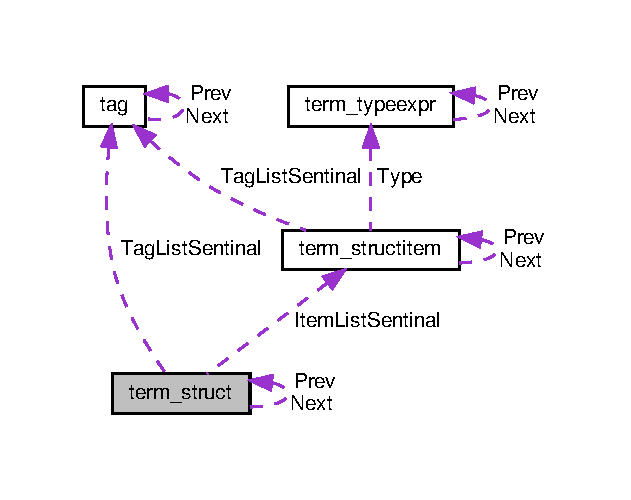
\includegraphics[width=305pt]{df/d72/structterm__struct__coll__graph}
\end{center}
\end{figure}
\doxysubsection*{Public Attributes}
\begin{DoxyCompactItemize}
\item 
abs\+\_\+stringptr \mbox{\hyperlink{structterm__struct_a89d9cb121c9adf97d79fe1a2304c672a}{Name}}
\item 
\mbox{\hyperlink{structtag}{tag}} \mbox{\hyperlink{structterm__struct_a95c474434ab1c1d7e1ac66df37592d68}{Tag\+List\+Sentinal}}
\item 
\mbox{\hyperlink{structterm__structitem}{term\+\_\+structitem}} \mbox{\hyperlink{structterm__struct_a0983a4cdc7024100a2f870b0d484a99d}{Item\+List\+Sentinal}}
\item 
u32 \mbox{\hyperlink{structterm__struct_a7346270cfcb97d2aba636aaccf0a35be}{Item\+Count}}
\item 
\mbox{\hyperlink{structterm__struct}{term\+\_\+struct}} $\ast$ \mbox{\hyperlink{structterm__struct_a733a9fd60e2c6d6dd108fe88e18a8cb8}{Next}}
\item 
\mbox{\hyperlink{structterm__struct}{term\+\_\+struct}} $\ast$ \mbox{\hyperlink{structterm__struct_aa5cc89c03d6af0b5a43680485f5224cb}{Prev}}
\end{DoxyCompactItemize}


\doxysubsection{Member Data Documentation}
\mbox{\Hypertarget{structterm__struct_a7346270cfcb97d2aba636aaccf0a35be}\label{structterm__struct_a7346270cfcb97d2aba636aaccf0a35be}} 
\index{term\_struct@{term\_struct}!ItemCount@{ItemCount}}
\index{ItemCount@{ItemCount}!term\_struct@{term\_struct}}
\doxysubsubsection{\texorpdfstring{ItemCount}{ItemCount}}
{\footnotesize\ttfamily u32 term\+\_\+struct\+::\+Item\+Count}

\mbox{\Hypertarget{structterm__struct_a0983a4cdc7024100a2f870b0d484a99d}\label{structterm__struct_a0983a4cdc7024100a2f870b0d484a99d}} 
\index{term\_struct@{term\_struct}!ItemListSentinal@{ItemListSentinal}}
\index{ItemListSentinal@{ItemListSentinal}!term\_struct@{term\_struct}}
\doxysubsubsection{\texorpdfstring{ItemListSentinal}{ItemListSentinal}}
{\footnotesize\ttfamily \mbox{\hyperlink{structterm__structitem}{term\+\_\+structitem}} term\+\_\+struct\+::\+Item\+List\+Sentinal}

\mbox{\Hypertarget{structterm__struct_a89d9cb121c9adf97d79fe1a2304c672a}\label{structterm__struct_a89d9cb121c9adf97d79fe1a2304c672a}} 
\index{term\_struct@{term\_struct}!Name@{Name}}
\index{Name@{Name}!term\_struct@{term\_struct}}
\doxysubsubsection{\texorpdfstring{Name}{Name}}
{\footnotesize\ttfamily abs\+\_\+stringptr term\+\_\+struct\+::\+Name}

\mbox{\Hypertarget{structterm__struct_a733a9fd60e2c6d6dd108fe88e18a8cb8}\label{structterm__struct_a733a9fd60e2c6d6dd108fe88e18a8cb8}} 
\index{term\_struct@{term\_struct}!Next@{Next}}
\index{Next@{Next}!term\_struct@{term\_struct}}
\doxysubsubsection{\texorpdfstring{Next}{Next}}
{\footnotesize\ttfamily \mbox{\hyperlink{structterm__struct}{term\+\_\+struct}}$\ast$ term\+\_\+struct\+::\+Next}

\mbox{\Hypertarget{structterm__struct_aa5cc89c03d6af0b5a43680485f5224cb}\label{structterm__struct_aa5cc89c03d6af0b5a43680485f5224cb}} 
\index{term\_struct@{term\_struct}!Prev@{Prev}}
\index{Prev@{Prev}!term\_struct@{term\_struct}}
\doxysubsubsection{\texorpdfstring{Prev}{Prev}}
{\footnotesize\ttfamily \mbox{\hyperlink{structterm__struct}{term\+\_\+struct}}$\ast$ term\+\_\+struct\+::\+Prev}

\mbox{\Hypertarget{structterm__struct_a95c474434ab1c1d7e1ac66df37592d68}\label{structterm__struct_a95c474434ab1c1d7e1ac66df37592d68}} 
\index{term\_struct@{term\_struct}!TagListSentinal@{TagListSentinal}}
\index{TagListSentinal@{TagListSentinal}!term\_struct@{term\_struct}}
\doxysubsubsection{\texorpdfstring{TagListSentinal}{TagListSentinal}}
{\footnotesize\ttfamily \mbox{\hyperlink{structtag}{tag}} term\+\_\+struct\+::\+Tag\+List\+Sentinal}



The documentation for this struct was generated from the following file\+:\begin{DoxyCompactItemize}
\item 
\mbox{\hyperlink{ab__parser_8h}{ab\+\_\+parser.\+h}}\end{DoxyCompactItemize}

\hypertarget{structterm__structitem}{}\doxysection{term\+\_\+structitem Struct Reference}
\label{structterm__structitem}\index{term\_structitem@{term\_structitem}}


{\ttfamily \#include $<$ab\+\_\+parser.\+h$>$}



Collaboration diagram for term\+\_\+structitem\+:
\nopagebreak
\begin{figure}[H]
\begin{center}
\leavevmode
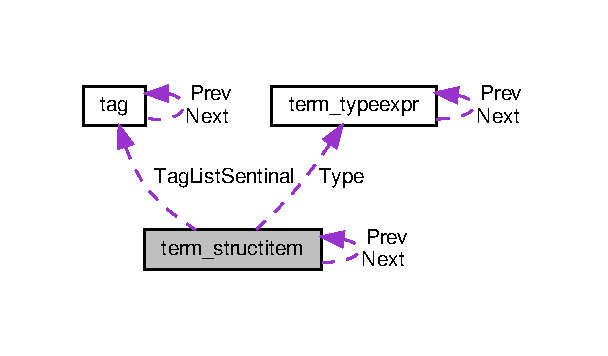
\includegraphics[width=294pt]{df/d30/structterm__structitem__coll__graph}
\end{center}
\end{figure}
\doxysubsection*{Public Attributes}
\begin{DoxyCompactItemize}
\item 
\mbox{\hyperlink{structterm__typeexpr}{term\+\_\+typeexpr}} $\ast$ \mbox{\hyperlink{structterm__structitem_ac2a7c2261f1714cedb33376eb440e66c}{Type}}
\item 
\mbox{\hyperlink{structtag}{tag}} \mbox{\hyperlink{structterm__structitem_a25c03f6130b24c035dadd65fbe5f0110}{Tag\+List\+Sentinal}}
\item 
\mbox{\hyperlink{structterm__structitem}{term\+\_\+structitem}} $\ast$ \mbox{\hyperlink{structterm__structitem_a92becd37fab5b7e4b326e3111c6a7c40}{Next}}
\item 
\mbox{\hyperlink{structterm__structitem}{term\+\_\+structitem}} $\ast$ \mbox{\hyperlink{structterm__structitem_a724d81ad66a76f54b153a97a8b175b7d}{Prev}}
\end{DoxyCompactItemize}


\doxysubsection{Member Data Documentation}
\mbox{\Hypertarget{structterm__structitem_a92becd37fab5b7e4b326e3111c6a7c40}\label{structterm__structitem_a92becd37fab5b7e4b326e3111c6a7c40}} 
\index{term\_structitem@{term\_structitem}!Next@{Next}}
\index{Next@{Next}!term\_structitem@{term\_structitem}}
\doxysubsubsection{\texorpdfstring{Next}{Next}}
{\footnotesize\ttfamily \mbox{\hyperlink{structterm__structitem}{term\+\_\+structitem}}$\ast$ term\+\_\+structitem\+::\+Next}

\mbox{\Hypertarget{structterm__structitem_a724d81ad66a76f54b153a97a8b175b7d}\label{structterm__structitem_a724d81ad66a76f54b153a97a8b175b7d}} 
\index{term\_structitem@{term\_structitem}!Prev@{Prev}}
\index{Prev@{Prev}!term\_structitem@{term\_structitem}}
\doxysubsubsection{\texorpdfstring{Prev}{Prev}}
{\footnotesize\ttfamily \mbox{\hyperlink{structterm__structitem}{term\+\_\+structitem}}$\ast$ term\+\_\+structitem\+::\+Prev}

\mbox{\Hypertarget{structterm__structitem_a25c03f6130b24c035dadd65fbe5f0110}\label{structterm__structitem_a25c03f6130b24c035dadd65fbe5f0110}} 
\index{term\_structitem@{term\_structitem}!TagListSentinal@{TagListSentinal}}
\index{TagListSentinal@{TagListSentinal}!term\_structitem@{term\_structitem}}
\doxysubsubsection{\texorpdfstring{TagListSentinal}{TagListSentinal}}
{\footnotesize\ttfamily \mbox{\hyperlink{structtag}{tag}} term\+\_\+structitem\+::\+Tag\+List\+Sentinal}

\mbox{\Hypertarget{structterm__structitem_ac2a7c2261f1714cedb33376eb440e66c}\label{structterm__structitem_ac2a7c2261f1714cedb33376eb440e66c}} 
\index{term\_structitem@{term\_structitem}!Type@{Type}}
\index{Type@{Type}!term\_structitem@{term\_structitem}}
\doxysubsubsection{\texorpdfstring{Type}{Type}}
{\footnotesize\ttfamily \mbox{\hyperlink{structterm__typeexpr}{term\+\_\+typeexpr}}$\ast$ term\+\_\+structitem\+::\+Type}



The documentation for this struct was generated from the following file\+:\begin{DoxyCompactItemize}
\item 
\mbox{\hyperlink{ab__parser_8h}{ab\+\_\+parser.\+h}}\end{DoxyCompactItemize}

\hypertarget{structterm__typeexpr}{}\doxysection{term\+\_\+typeexpr Struct Reference}
\label{structterm__typeexpr}\index{term\_typeexpr@{term\_typeexpr}}


{\ttfamily \#include $<$ab\+\_\+parser.\+h$>$}



Collaboration diagram for term\+\_\+typeexpr\+:\nopagebreak
\begin{figure}[H]
\begin{center}
\leavevmode
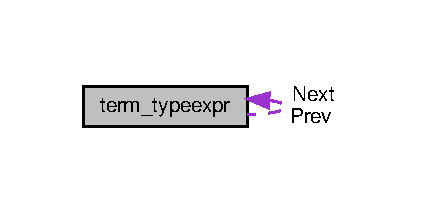
\includegraphics[width=202pt]{db/de8/structterm__typeexpr__coll__graph}
\end{center}
\end{figure}
\doxysubsection*{Public Attributes}
\begin{DoxyCompactItemize}
\item 
st\+\_\+ptr \mbox{\hyperlink{structterm__typeexpr_aa33dcc1345202efe5929d00019e226e5}{Type}}
\item 
st\+\_\+ptr \mbox{\hyperlink{structterm__typeexpr_a2510ec68bc76b3b2aa7a6391018750bc}{Name}}
\item 
b8 \mbox{\hyperlink{structterm__typeexpr_a93ac336807d6f45f5bd6270f21b02679}{is\+Ptr}}
\item 
b8 \mbox{\hyperlink{structterm__typeexpr_aa8779ec62ac26dd1239060953fd65f56}{is\+Reference}}
\item 
b8 \mbox{\hyperlink{structterm__typeexpr_af67982c68088bdca49bdcd1738bb7b7a}{is\+Const}}
\item 
b8 \mbox{\hyperlink{structterm__typeexpr_a2bc07d643069855d995bbcd4fa81006c}{is\+Array}}
\item 
s32 \mbox{\hyperlink{structterm__typeexpr_ab93773f58c02499d82f1dd1188182506}{Array\+Length}}
\item 
\mbox{\hyperlink{ab__parser_8h_ac9039717ce4cccacf493ee306650a423}{custom\+\_\+type}} \mbox{\hyperlink{structterm__typeexpr_a9544ece5f851486a3a725c0bd87df73f}{Custom\+Type}}
\item 
\mbox{\hyperlink{structterm__typeexpr}{term\+\_\+typeexpr}} $\ast$ \mbox{\hyperlink{structterm__typeexpr_a827f986754feb8a31cb88bb5929f35cb}{Next}}
\item 
\mbox{\hyperlink{structterm__typeexpr}{term\+\_\+typeexpr}} $\ast$ \mbox{\hyperlink{structterm__typeexpr_ac489d3375eb8507325fd21d328bdf2cc}{Prev}}
\end{DoxyCompactItemize}


\doxysubsection{Member Data Documentation}
\mbox{\Hypertarget{structterm__typeexpr_ab93773f58c02499d82f1dd1188182506}\label{structterm__typeexpr_ab93773f58c02499d82f1dd1188182506}} 
\index{term\_typeexpr@{term\_typeexpr}!ArrayLength@{ArrayLength}}
\index{ArrayLength@{ArrayLength}!term\_typeexpr@{term\_typeexpr}}
\doxysubsubsection{\texorpdfstring{ArrayLength}{ArrayLength}}
{\footnotesize\ttfamily s32 term\+\_\+typeexpr\+::\+Array\+Length}

\mbox{\Hypertarget{structterm__typeexpr_a9544ece5f851486a3a725c0bd87df73f}\label{structterm__typeexpr_a9544ece5f851486a3a725c0bd87df73f}} 
\index{term\_typeexpr@{term\_typeexpr}!CustomType@{CustomType}}
\index{CustomType@{CustomType}!term\_typeexpr@{term\_typeexpr}}
\doxysubsubsection{\texorpdfstring{CustomType}{CustomType}}
{\footnotesize\ttfamily \mbox{\hyperlink{ab__parser_8h_ac9039717ce4cccacf493ee306650a423}{custom\+\_\+type}} term\+\_\+typeexpr\+::\+Custom\+Type}

\mbox{\Hypertarget{structterm__typeexpr_a2bc07d643069855d995bbcd4fa81006c}\label{structterm__typeexpr_a2bc07d643069855d995bbcd4fa81006c}} 
\index{term\_typeexpr@{term\_typeexpr}!isArray@{isArray}}
\index{isArray@{isArray}!term\_typeexpr@{term\_typeexpr}}
\doxysubsubsection{\texorpdfstring{isArray}{isArray}}
{\footnotesize\ttfamily b8 term\+\_\+typeexpr\+::is\+Array}

\mbox{\Hypertarget{structterm__typeexpr_af67982c68088bdca49bdcd1738bb7b7a}\label{structterm__typeexpr_af67982c68088bdca49bdcd1738bb7b7a}} 
\index{term\_typeexpr@{term\_typeexpr}!isConst@{isConst}}
\index{isConst@{isConst}!term\_typeexpr@{term\_typeexpr}}
\doxysubsubsection{\texorpdfstring{isConst}{isConst}}
{\footnotesize\ttfamily b8 term\+\_\+typeexpr\+::is\+Const}

\mbox{\Hypertarget{structterm__typeexpr_a93ac336807d6f45f5bd6270f21b02679}\label{structterm__typeexpr_a93ac336807d6f45f5bd6270f21b02679}} 
\index{term\_typeexpr@{term\_typeexpr}!isPtr@{isPtr}}
\index{isPtr@{isPtr}!term\_typeexpr@{term\_typeexpr}}
\doxysubsubsection{\texorpdfstring{isPtr}{isPtr}}
{\footnotesize\ttfamily b8 term\+\_\+typeexpr\+::is\+Ptr}

\mbox{\Hypertarget{structterm__typeexpr_aa8779ec62ac26dd1239060953fd65f56}\label{structterm__typeexpr_aa8779ec62ac26dd1239060953fd65f56}} 
\index{term\_typeexpr@{term\_typeexpr}!isReference@{isReference}}
\index{isReference@{isReference}!term\_typeexpr@{term\_typeexpr}}
\doxysubsubsection{\texorpdfstring{isReference}{isReference}}
{\footnotesize\ttfamily b8 term\+\_\+typeexpr\+::is\+Reference}

\mbox{\Hypertarget{structterm__typeexpr_a2510ec68bc76b3b2aa7a6391018750bc}\label{structterm__typeexpr_a2510ec68bc76b3b2aa7a6391018750bc}} 
\index{term\_typeexpr@{term\_typeexpr}!Name@{Name}}
\index{Name@{Name}!term\_typeexpr@{term\_typeexpr}}
\doxysubsubsection{\texorpdfstring{Name}{Name}}
{\footnotesize\ttfamily st\+\_\+ptr term\+\_\+typeexpr\+::\+Name}

\mbox{\Hypertarget{structterm__typeexpr_a827f986754feb8a31cb88bb5929f35cb}\label{structterm__typeexpr_a827f986754feb8a31cb88bb5929f35cb}} 
\index{term\_typeexpr@{term\_typeexpr}!Next@{Next}}
\index{Next@{Next}!term\_typeexpr@{term\_typeexpr}}
\doxysubsubsection{\texorpdfstring{Next}{Next}}
{\footnotesize\ttfamily \mbox{\hyperlink{structterm__typeexpr}{term\+\_\+typeexpr}}$\ast$ term\+\_\+typeexpr\+::\+Next}

\mbox{\Hypertarget{structterm__typeexpr_ac489d3375eb8507325fd21d328bdf2cc}\label{structterm__typeexpr_ac489d3375eb8507325fd21d328bdf2cc}} 
\index{term\_typeexpr@{term\_typeexpr}!Prev@{Prev}}
\index{Prev@{Prev}!term\_typeexpr@{term\_typeexpr}}
\doxysubsubsection{\texorpdfstring{Prev}{Prev}}
{\footnotesize\ttfamily \mbox{\hyperlink{structterm__typeexpr}{term\+\_\+typeexpr}}$\ast$ term\+\_\+typeexpr\+::\+Prev}

\mbox{\Hypertarget{structterm__typeexpr_aa33dcc1345202efe5929d00019e226e5}\label{structterm__typeexpr_aa33dcc1345202efe5929d00019e226e5}} 
\index{term\_typeexpr@{term\_typeexpr}!Type@{Type}}
\index{Type@{Type}!term\_typeexpr@{term\_typeexpr}}
\doxysubsubsection{\texorpdfstring{Type}{Type}}
{\footnotesize\ttfamily st\+\_\+ptr term\+\_\+typeexpr\+::\+Type}



The documentation for this struct was generated from the following file\+:\begin{DoxyCompactItemize}
\item 
\mbox{\hyperlink{ab__parser_8h}{ab\+\_\+parser.\+h}}\end{DoxyCompactItemize}

\hypertarget{structtest__cmd__queue}{}\section{test\+\_\+cmd\+\_\+queue Struct Reference}
\label{structtest__cmd__queue}\index{test\+\_\+cmd\+\_\+queue@{test\+\_\+cmd\+\_\+queue}}


A circular queue of 10 elements for the state command test\+\_\+cmd.  




{\ttfamily \#include $<$Generated\+\_\+\+Test.\+h$>$}

\subsection*{Public Attributes}
\begin{DoxyCompactItemize}
\item 
\hyperlink{PreprocTest_8h_a55ed691059222a58555cf9992ec14431}{test\+\_\+cmd} \hyperlink{structtest__cmd__queue_a893fe182353a750337200b5aad9bacb3}{Items} \mbox{[}10\mbox{]}
\item 
s32 \hyperlink{structtest__cmd__queue_a20ed55b6b8b836106c001539d2e3d599}{Front}
\item 
s32 \hyperlink{structtest__cmd__queue_a7cedef36f33507cbadf3f4ef95aa7cec}{Rear}
\end{DoxyCompactItemize}


\subsection{Detailed Description}
A circular queue of 10 elements for the state command test\+\_\+cmd. 

\subsection{Member Data Documentation}
\mbox{\Hypertarget{structtest__cmd__queue_a20ed55b6b8b836106c001539d2e3d599}\label{structtest__cmd__queue_a20ed55b6b8b836106c001539d2e3d599}} 
\index{test\+\_\+cmd\+\_\+queue@{test\+\_\+cmd\+\_\+queue}!Front@{Front}}
\index{Front@{Front}!test\+\_\+cmd\+\_\+queue@{test\+\_\+cmd\+\_\+queue}}
\subsubsection{\texorpdfstring{Front}{Front}}
{\footnotesize\ttfamily s32 test\+\_\+cmd\+\_\+queue\+::\+Front}

\mbox{\Hypertarget{structtest__cmd__queue_a893fe182353a750337200b5aad9bacb3}\label{structtest__cmd__queue_a893fe182353a750337200b5aad9bacb3}} 
\index{test\+\_\+cmd\+\_\+queue@{test\+\_\+cmd\+\_\+queue}!Items@{Items}}
\index{Items@{Items}!test\+\_\+cmd\+\_\+queue@{test\+\_\+cmd\+\_\+queue}}
\subsubsection{\texorpdfstring{Items}{Items}}
{\footnotesize\ttfamily \hyperlink{PreprocTest_8h_a55ed691059222a58555cf9992ec14431}{test\+\_\+cmd} test\+\_\+cmd\+\_\+queue\+::\+Items\mbox{[}10\mbox{]}}

\mbox{\Hypertarget{structtest__cmd__queue_a7cedef36f33507cbadf3f4ef95aa7cec}\label{structtest__cmd__queue_a7cedef36f33507cbadf3f4ef95aa7cec}} 
\index{test\+\_\+cmd\+\_\+queue@{test\+\_\+cmd\+\_\+queue}!Rear@{Rear}}
\index{Rear@{Rear}!test\+\_\+cmd\+\_\+queue@{test\+\_\+cmd\+\_\+queue}}
\subsubsection{\texorpdfstring{Rear}{Rear}}
{\footnotesize\ttfamily s32 test\+\_\+cmd\+\_\+queue\+::\+Rear}



The documentation for this struct was generated from the following file\+:\begin{DoxyCompactItemize}
\item 
\hyperlink{Generated__Test_8h}{Generated\+\_\+\+Test.\+h}\end{DoxyCompactItemize}

\hypertarget{structtest__suite__token__list__item}{}\section{test\+\_\+suite\+\_\+token\+\_\+list\+\_\+item Struct Reference}
\label{structtest__suite__token__list__item}\index{test\+\_\+suite\+\_\+token\+\_\+list\+\_\+item@{test\+\_\+suite\+\_\+token\+\_\+list\+\_\+item}}


Collaboration diagram for test\+\_\+suite\+\_\+token\+\_\+list\+\_\+item\+:
\nopagebreak
\begin{figure}[H]
\begin{center}
\leavevmode
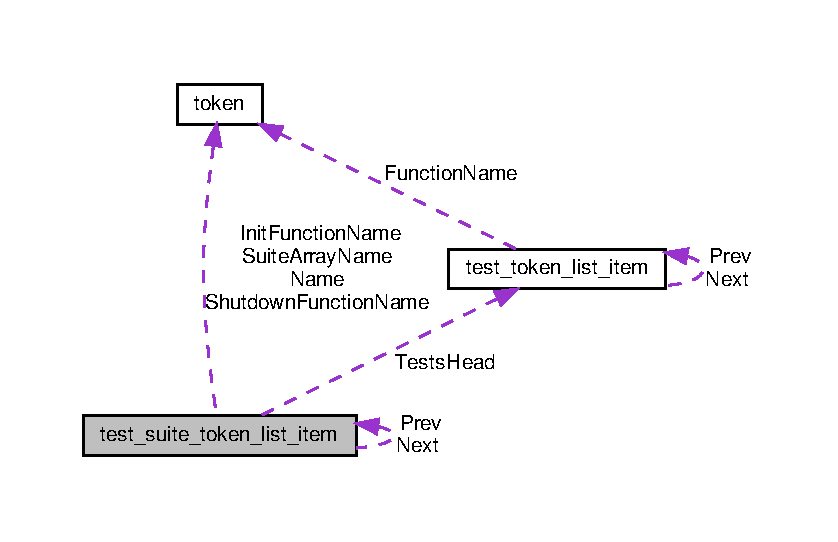
\includegraphics[width=350pt]{da/d06/structtest__suite__token__list__item__coll__graph}
\end{center}
\end{figure}
\subsection*{Public Attributes}
\begin{DoxyCompactItemize}
\item 
\hyperlink{structtoken}{token} \hyperlink{structtest__suite__token__list__item_a63834f736499a8eb9a5be4ce658ad420}{Name}
\item 
\hyperlink{structtoken}{token} \hyperlink{structtest__suite__token__list__item_a33bab1f9cd9b0c869eadfcbde0320d86}{Suite\+Array\+Name}
\item 
\hyperlink{structtoken}{token} \hyperlink{structtest__suite__token__list__item_a3d7b2baf23150725e91f919067ec6d81}{Init\+Function\+Name}
\item 
\hyperlink{structtoken}{token} \hyperlink{structtest__suite__token__list__item_a0577805f0d8627a70a98882765c9a2b9}{Shutdown\+Function\+Name}
\item 
\hyperlink{structtest__token__list__item}{test\+\_\+token\+\_\+list\+\_\+item} \hyperlink{structtest__suite__token__list__item_a733adf7402d148f6d1d713f7ad08b835}{Tests\+Head}
\item 
\hyperlink{structtest__suite__token__list__item}{test\+\_\+suite\+\_\+token\+\_\+list\+\_\+item} $\ast$ \hyperlink{structtest__suite__token__list__item_aa9d98f0ebaaa60117452f83b01a5f875}{Next}
\item 
\hyperlink{structtest__suite__token__list__item}{test\+\_\+suite\+\_\+token\+\_\+list\+\_\+item} $\ast$ \hyperlink{structtest__suite__token__list__item_a0bbc26a13de896100669c60385883fd2}{Prev}
\end{DoxyCompactItemize}


\subsection{Member Data Documentation}
\mbox{\Hypertarget{structtest__suite__token__list__item_a3d7b2baf23150725e91f919067ec6d81}\label{structtest__suite__token__list__item_a3d7b2baf23150725e91f919067ec6d81}} 
\index{test\+\_\+suite\+\_\+token\+\_\+list\+\_\+item@{test\+\_\+suite\+\_\+token\+\_\+list\+\_\+item}!Init\+Function\+Name@{Init\+Function\+Name}}
\index{Init\+Function\+Name@{Init\+Function\+Name}!test\+\_\+suite\+\_\+token\+\_\+list\+\_\+item@{test\+\_\+suite\+\_\+token\+\_\+list\+\_\+item}}
\subsubsection{\texorpdfstring{Init\+Function\+Name}{InitFunctionName}}
{\footnotesize\ttfamily \hyperlink{structtoken}{token} test\+\_\+suite\+\_\+token\+\_\+list\+\_\+item\+::\+Init\+Function\+Name}

\mbox{\Hypertarget{structtest__suite__token__list__item_a63834f736499a8eb9a5be4ce658ad420}\label{structtest__suite__token__list__item_a63834f736499a8eb9a5be4ce658ad420}} 
\index{test\+\_\+suite\+\_\+token\+\_\+list\+\_\+item@{test\+\_\+suite\+\_\+token\+\_\+list\+\_\+item}!Name@{Name}}
\index{Name@{Name}!test\+\_\+suite\+\_\+token\+\_\+list\+\_\+item@{test\+\_\+suite\+\_\+token\+\_\+list\+\_\+item}}
\subsubsection{\texorpdfstring{Name}{Name}}
{\footnotesize\ttfamily \hyperlink{structtoken}{token} test\+\_\+suite\+\_\+token\+\_\+list\+\_\+item\+::\+Name}

\mbox{\Hypertarget{structtest__suite__token__list__item_aa9d98f0ebaaa60117452f83b01a5f875}\label{structtest__suite__token__list__item_aa9d98f0ebaaa60117452f83b01a5f875}} 
\index{test\+\_\+suite\+\_\+token\+\_\+list\+\_\+item@{test\+\_\+suite\+\_\+token\+\_\+list\+\_\+item}!Next@{Next}}
\index{Next@{Next}!test\+\_\+suite\+\_\+token\+\_\+list\+\_\+item@{test\+\_\+suite\+\_\+token\+\_\+list\+\_\+item}}
\subsubsection{\texorpdfstring{Next}{Next}}
{\footnotesize\ttfamily \hyperlink{structtest__suite__token__list__item}{test\+\_\+suite\+\_\+token\+\_\+list\+\_\+item}$\ast$ test\+\_\+suite\+\_\+token\+\_\+list\+\_\+item\+::\+Next}

\mbox{\Hypertarget{structtest__suite__token__list__item_a0bbc26a13de896100669c60385883fd2}\label{structtest__suite__token__list__item_a0bbc26a13de896100669c60385883fd2}} 
\index{test\+\_\+suite\+\_\+token\+\_\+list\+\_\+item@{test\+\_\+suite\+\_\+token\+\_\+list\+\_\+item}!Prev@{Prev}}
\index{Prev@{Prev}!test\+\_\+suite\+\_\+token\+\_\+list\+\_\+item@{test\+\_\+suite\+\_\+token\+\_\+list\+\_\+item}}
\subsubsection{\texorpdfstring{Prev}{Prev}}
{\footnotesize\ttfamily \hyperlink{structtest__suite__token__list__item}{test\+\_\+suite\+\_\+token\+\_\+list\+\_\+item}$\ast$ test\+\_\+suite\+\_\+token\+\_\+list\+\_\+item\+::\+Prev}

\mbox{\Hypertarget{structtest__suite__token__list__item_a0577805f0d8627a70a98882765c9a2b9}\label{structtest__suite__token__list__item_a0577805f0d8627a70a98882765c9a2b9}} 
\index{test\+\_\+suite\+\_\+token\+\_\+list\+\_\+item@{test\+\_\+suite\+\_\+token\+\_\+list\+\_\+item}!Shutdown\+Function\+Name@{Shutdown\+Function\+Name}}
\index{Shutdown\+Function\+Name@{Shutdown\+Function\+Name}!test\+\_\+suite\+\_\+token\+\_\+list\+\_\+item@{test\+\_\+suite\+\_\+token\+\_\+list\+\_\+item}}
\subsubsection{\texorpdfstring{Shutdown\+Function\+Name}{ShutdownFunctionName}}
{\footnotesize\ttfamily \hyperlink{structtoken}{token} test\+\_\+suite\+\_\+token\+\_\+list\+\_\+item\+::\+Shutdown\+Function\+Name}

\mbox{\Hypertarget{structtest__suite__token__list__item_a33bab1f9cd9b0c869eadfcbde0320d86}\label{structtest__suite__token__list__item_a33bab1f9cd9b0c869eadfcbde0320d86}} 
\index{test\+\_\+suite\+\_\+token\+\_\+list\+\_\+item@{test\+\_\+suite\+\_\+token\+\_\+list\+\_\+item}!Suite\+Array\+Name@{Suite\+Array\+Name}}
\index{Suite\+Array\+Name@{Suite\+Array\+Name}!test\+\_\+suite\+\_\+token\+\_\+list\+\_\+item@{test\+\_\+suite\+\_\+token\+\_\+list\+\_\+item}}
\subsubsection{\texorpdfstring{Suite\+Array\+Name}{SuiteArrayName}}
{\footnotesize\ttfamily \hyperlink{structtoken}{token} test\+\_\+suite\+\_\+token\+\_\+list\+\_\+item\+::\+Suite\+Array\+Name}

\mbox{\Hypertarget{structtest__suite__token__list__item_a733adf7402d148f6d1d713f7ad08b835}\label{structtest__suite__token__list__item_a733adf7402d148f6d1d713f7ad08b835}} 
\index{test\+\_\+suite\+\_\+token\+\_\+list\+\_\+item@{test\+\_\+suite\+\_\+token\+\_\+list\+\_\+item}!Tests\+Head@{Tests\+Head}}
\index{Tests\+Head@{Tests\+Head}!test\+\_\+suite\+\_\+token\+\_\+list\+\_\+item@{test\+\_\+suite\+\_\+token\+\_\+list\+\_\+item}}
\subsubsection{\texorpdfstring{Tests\+Head}{TestsHead}}
{\footnotesize\ttfamily \hyperlink{structtest__token__list__item}{test\+\_\+token\+\_\+list\+\_\+item} test\+\_\+suite\+\_\+token\+\_\+list\+\_\+item\+::\+Tests\+Head}



The documentation for this struct was generated from the following file\+:\begin{DoxyCompactItemize}
\item 
\hyperlink{test__preprocessor_8cpp}{test\+\_\+preprocessor.\+cpp}\end{DoxyCompactItemize}

\hypertarget{structtest__token__list__item}{}\section{test\+\_\+token\+\_\+list\+\_\+item Struct Reference}
\label{structtest__token__list__item}\index{test\+\_\+token\+\_\+list\+\_\+item@{test\+\_\+token\+\_\+list\+\_\+item}}


Collaboration diagram for test\+\_\+token\+\_\+list\+\_\+item\+:\nopagebreak
\begin{figure}[H]
\begin{center}
\leavevmode
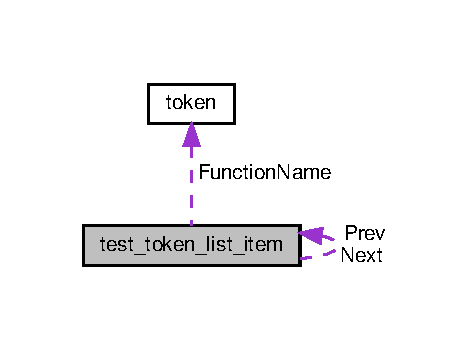
\includegraphics[width=226pt]{d0/d11/structtest__token__list__item__coll__graph}
\end{center}
\end{figure}
\subsection*{Public Attributes}
\begin{DoxyCompactItemize}
\item 
\hyperlink{structtoken}{token} \hyperlink{structtest__token__list__item_a48319a908d351d150a224fd1ece758d7}{Function\+Name}
\item 
token\+\_\+list\+\_\+item \hyperlink{structtest__token__list__item_a30e55573c651ec80614b75f9b180dc80}{Test\+Steps\+Head}
\item 
\hyperlink{structtest__token__list__item}{test\+\_\+token\+\_\+list\+\_\+item} $\ast$ \hyperlink{structtest__token__list__item_a271ea32ddd03b4f6bb44237881915692}{Next}
\item 
\hyperlink{structtest__token__list__item}{test\+\_\+token\+\_\+list\+\_\+item} $\ast$ \hyperlink{structtest__token__list__item_aa053b5098e750d72759f6520d287c74d}{Prev}
\end{DoxyCompactItemize}


\subsection{Member Data Documentation}
\mbox{\Hypertarget{structtest__token__list__item_a48319a908d351d150a224fd1ece758d7}\label{structtest__token__list__item_a48319a908d351d150a224fd1ece758d7}} 
\index{test\+\_\+token\+\_\+list\+\_\+item@{test\+\_\+token\+\_\+list\+\_\+item}!Function\+Name@{Function\+Name}}
\index{Function\+Name@{Function\+Name}!test\+\_\+token\+\_\+list\+\_\+item@{test\+\_\+token\+\_\+list\+\_\+item}}
\subsubsection{\texorpdfstring{Function\+Name}{FunctionName}}
{\footnotesize\ttfamily \hyperlink{structtoken}{token} test\+\_\+token\+\_\+list\+\_\+item\+::\+Function\+Name}

\mbox{\Hypertarget{structtest__token__list__item_a271ea32ddd03b4f6bb44237881915692}\label{structtest__token__list__item_a271ea32ddd03b4f6bb44237881915692}} 
\index{test\+\_\+token\+\_\+list\+\_\+item@{test\+\_\+token\+\_\+list\+\_\+item}!Next@{Next}}
\index{Next@{Next}!test\+\_\+token\+\_\+list\+\_\+item@{test\+\_\+token\+\_\+list\+\_\+item}}
\subsubsection{\texorpdfstring{Next}{Next}}
{\footnotesize\ttfamily \hyperlink{structtest__token__list__item}{test\+\_\+token\+\_\+list\+\_\+item}$\ast$ test\+\_\+token\+\_\+list\+\_\+item\+::\+Next}

\mbox{\Hypertarget{structtest__token__list__item_aa053b5098e750d72759f6520d287c74d}\label{structtest__token__list__item_aa053b5098e750d72759f6520d287c74d}} 
\index{test\+\_\+token\+\_\+list\+\_\+item@{test\+\_\+token\+\_\+list\+\_\+item}!Prev@{Prev}}
\index{Prev@{Prev}!test\+\_\+token\+\_\+list\+\_\+item@{test\+\_\+token\+\_\+list\+\_\+item}}
\subsubsection{\texorpdfstring{Prev}{Prev}}
{\footnotesize\ttfamily \hyperlink{structtest__token__list__item}{test\+\_\+token\+\_\+list\+\_\+item}$\ast$ test\+\_\+token\+\_\+list\+\_\+item\+::\+Prev}

\mbox{\Hypertarget{structtest__token__list__item_a30e55573c651ec80614b75f9b180dc80}\label{structtest__token__list__item_a30e55573c651ec80614b75f9b180dc80}} 
\index{test\+\_\+token\+\_\+list\+\_\+item@{test\+\_\+token\+\_\+list\+\_\+item}!Test\+Steps\+Head@{Test\+Steps\+Head}}
\index{Test\+Steps\+Head@{Test\+Steps\+Head}!test\+\_\+token\+\_\+list\+\_\+item@{test\+\_\+token\+\_\+list\+\_\+item}}
\subsubsection{\texorpdfstring{Test\+Steps\+Head}{TestStepsHead}}
{\footnotesize\ttfamily token\+\_\+list\+\_\+item test\+\_\+token\+\_\+list\+\_\+item\+::\+Test\+Steps\+Head}



The documentation for this struct was generated from the following file\+:\begin{DoxyCompactItemize}
\item 
\hyperlink{test__preprocessor_8cpp}{test\+\_\+preprocessor.\+cpp}\end{DoxyCompactItemize}

\hypertarget{structtest__type}{}\doxysection{test\+\_\+type Struct Reference}
\label{structtest__type}\index{test\_type@{test\_type}}


{\ttfamily \#include $<$Preproc\+Test.\+h$>$}



Collaboration diagram for test\+\_\+type\+:\nopagebreak
\begin{figure}[H]
\begin{center}
\leavevmode
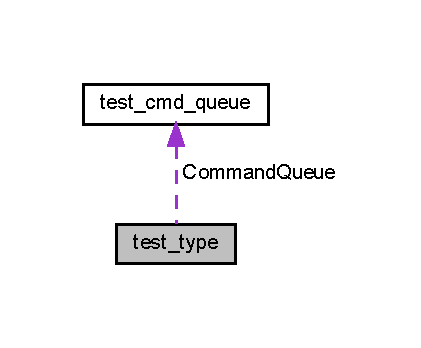
\includegraphics[width=202pt]{d5/dfe/structtest__type__coll__graph}
\end{center}
\end{figure}
\doxysubsection*{Public Attributes}
\begin{DoxyCompactItemize}
\item 
test\+\_\+statemachine $\ast$ \mbox{\hyperlink{structtest__type_a48139457e16e23a57531e5af02be7f14}{Current\+State}}
\item 
b8 \mbox{\hyperlink{structtest__type_a36eb3041ef1341aec27a2a2d98500ce6}{is\+New\+State}}
\item 
\mbox{\hyperlink{structtest__cmd__queue}{test\+\_\+cmd\+\_\+queue}} \mbox{\hyperlink{structtest__type_a9ef32b05c6f8a712062f8261d71665ca}{Command\+Queue}}
\end{DoxyCompactItemize}


\doxysubsection{Member Data Documentation}
\mbox{\Hypertarget{structtest__type_a9ef32b05c6f8a712062f8261d71665ca}\label{structtest__type_a9ef32b05c6f8a712062f8261d71665ca}} 
\index{test\_type@{test\_type}!CommandQueue@{CommandQueue}}
\index{CommandQueue@{CommandQueue}!test\_type@{test\_type}}
\doxysubsubsection{\texorpdfstring{CommandQueue}{CommandQueue}}
{\footnotesize\ttfamily \mbox{\hyperlink{structtest__cmd__queue}{test\+\_\+cmd\+\_\+queue}} test\+\_\+type\+::\+Command\+Queue}

\mbox{\Hypertarget{structtest__type_a48139457e16e23a57531e5af02be7f14}\label{structtest__type_a48139457e16e23a57531e5af02be7f14}} 
\index{test\_type@{test\_type}!CurrentState@{CurrentState}}
\index{CurrentState@{CurrentState}!test\_type@{test\_type}}
\doxysubsubsection{\texorpdfstring{CurrentState}{CurrentState}}
{\footnotesize\ttfamily test\+\_\+statemachine$\ast$ test\+\_\+type\+::\+Current\+State}

\mbox{\Hypertarget{structtest__type_a36eb3041ef1341aec27a2a2d98500ce6}\label{structtest__type_a36eb3041ef1341aec27a2a2d98500ce6}} 
\index{test\_type@{test\_type}!isNewState@{isNewState}}
\index{isNewState@{isNewState}!test\_type@{test\_type}}
\doxysubsubsection{\texorpdfstring{isNewState}{isNewState}}
{\footnotesize\ttfamily b8 test\+\_\+type\+::is\+New\+State}



The documentation for this struct was generated from the following file\+:\begin{DoxyCompactItemize}
\item 
\mbox{\hyperlink{PreprocTest_8h}{Preproc\+Test.\+h}}\end{DoxyCompactItemize}

\hypertarget{structtoken}{}\doxysection{token Struct Reference}
\label{structtoken}\index{token@{token}}


{\ttfamily \#include $<$ab\+\_\+lexer.\+h$>$}

\doxysubsection*{Public Attributes}
\begin{DoxyCompactItemize}
\item 
\mbox{\hyperlink{ab__lexer_8h_afe5ef662303b6b710ea6ee1a944bad0d}{token\+\_\+type}} \mbox{\hyperlink{structtoken_a82914c351900753f626fa2d6fcb12fde}{Type}}
\item 
abs\+\_\+stringptr \mbox{\hyperlink{structtoken_afe96285022144ed40a345ac60d688550}{Text}}
\end{DoxyCompactItemize}


\doxysubsection{Member Data Documentation}
\mbox{\Hypertarget{structtoken_afe96285022144ed40a345ac60d688550}\label{structtoken_afe96285022144ed40a345ac60d688550}} 
\index{token@{token}!Text@{Text}}
\index{Text@{Text}!token@{token}}
\doxysubsubsection{\texorpdfstring{Text}{Text}}
{\footnotesize\ttfamily abs\+\_\+stringptr token\+::\+Text}

\mbox{\Hypertarget{structtoken_a82914c351900753f626fa2d6fcb12fde}\label{structtoken_a82914c351900753f626fa2d6fcb12fde}} 
\index{token@{token}!Type@{Type}}
\index{Type@{Type}!token@{token}}
\doxysubsubsection{\texorpdfstring{Type}{Type}}
{\footnotesize\ttfamily \mbox{\hyperlink{ab__lexer_8h_afe5ef662303b6b710ea6ee1a944bad0d}{token\+\_\+type}} token\+::\+Type}



The documentation for this struct was generated from the following file\+:\begin{DoxyCompactItemize}
\item 
\mbox{\hyperlink{ab__lexer_8h}{ab\+\_\+lexer.\+h}}\end{DoxyCompactItemize}

\chapter{File Documentation}
\hypertarget{ab__lexer_8h}{}\doxysection{ab\+\_\+lexer.\+h File Reference}
\label{ab__lexer_8h}\index{ab\_lexer.h@{ab\_lexer.h}}
{\ttfamily \#include $<$stdlib.\+h$>$}\newline
{\ttfamily \#include \char`\"{}ab\+\_\+string.\+h\char`\"{}}\newline
{\ttfamily \#include \char`\"{}ab\+\_\+file.\+h\char`\"{}}\newline
Include dependency graph for ab\+\_\+lexer.\+h\+:
\nopagebreak
\begin{figure}[H]
\begin{center}
\leavevmode
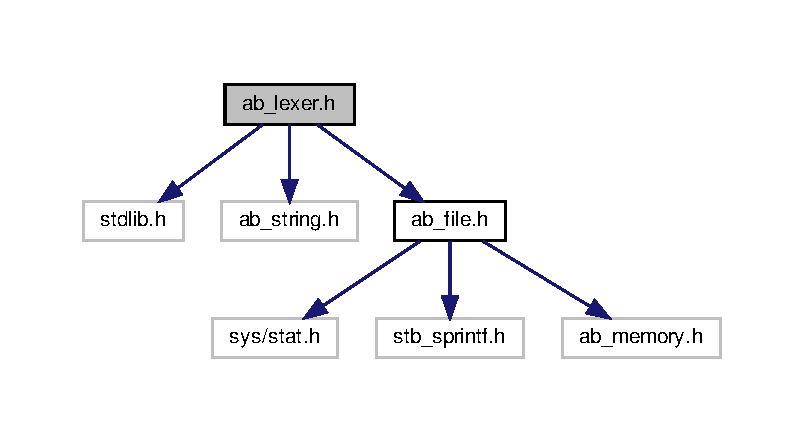
\includegraphics[width=350pt]{da/d7a/ab__lexer_8h__incl}
\end{center}
\end{figure}
This graph shows which files directly or indirectly include this file\+:
\nopagebreak
\begin{figure}[H]
\begin{center}
\leavevmode
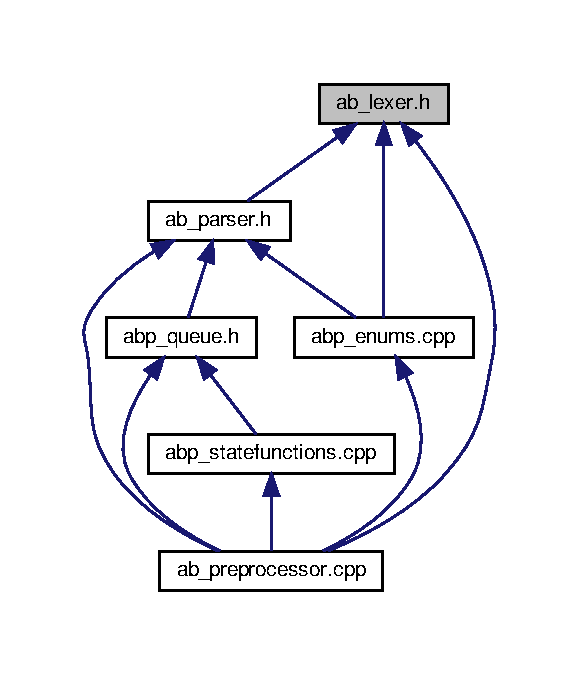
\includegraphics[width=350pt]{d7/d69/ab__lexer_8h__dep__incl}
\end{center}
\end{figure}
\doxysubsection*{Classes}
\begin{DoxyCompactItemize}
\item 
struct \mbox{\hyperlink{structtoken}{token}}
\item 
struct \mbox{\hyperlink{structlexer}{lexer}}
\end{DoxyCompactItemize}
\doxysubsection*{Enumerations}
\begin{DoxyCompactItemize}
\item 
enum \mbox{\hyperlink{ab__lexer_8h_afe5ef662303b6b710ea6ee1a944bad0d}{token\+\_\+type}} \{ \newline
\mbox{\hyperlink{ab__lexer_8h_afe5ef662303b6b710ea6ee1a944bad0da892829e561dc7befd1a48886ec9fafaf}{T\+O\+K\+E\+N\+\_\+\+Unknown}}, 
\mbox{\hyperlink{ab__lexer_8h_afe5ef662303b6b710ea6ee1a944bad0da461b56860fa20c58692816c64fbe3e82}{T\+O\+K\+E\+N\+\_\+\+Open\+Paren}}, 
\mbox{\hyperlink{ab__lexer_8h_afe5ef662303b6b710ea6ee1a944bad0dab194bde3d5b9eedc596b4e9c177a02bf}{T\+O\+K\+E\+N\+\_\+\+Close\+Paren}}, 
\mbox{\hyperlink{ab__lexer_8h_afe5ef662303b6b710ea6ee1a944bad0da844de61fbecc86df7402533595d0028e}{T\+O\+K\+E\+N\+\_\+\+Colon}}, 
\newline
\mbox{\hyperlink{ab__lexer_8h_afe5ef662303b6b710ea6ee1a944bad0da1e561e7c4db683063f655b59f48d8fa1}{T\+O\+K\+E\+N\+\_\+\+Semicolon}}, 
\mbox{\hyperlink{ab__lexer_8h_afe5ef662303b6b710ea6ee1a944bad0dad6aae4a41409c1b9e0ea73cc0896843b}{T\+O\+K\+E\+N\+\_\+\+Comma}}, 
\mbox{\hyperlink{ab__lexer_8h_afe5ef662303b6b710ea6ee1a944bad0da15a0aa1b1e93135757584ccd08634c5c}{T\+O\+K\+E\+N\+\_\+\+Asterisk}}, 
\mbox{\hyperlink{ab__lexer_8h_afe5ef662303b6b710ea6ee1a944bad0dafd406f033139bb6f609ace25a31c2f3a}{T\+O\+K\+E\+N\+\_\+\+Open\+Bracket}}, 
\newline
\mbox{\hyperlink{ab__lexer_8h_afe5ef662303b6b710ea6ee1a944bad0da3be38f6d9101f2361ffb117bde66e8b1}{T\+O\+K\+E\+N\+\_\+\+Close\+Bracket}}, 
\mbox{\hyperlink{ab__lexer_8h_afe5ef662303b6b710ea6ee1a944bad0da985f18bfc75b5bb16f6d8cd7ee3c5eef}{T\+O\+K\+E\+N\+\_\+\+Open\+Brace}}, 
\mbox{\hyperlink{ab__lexer_8h_afe5ef662303b6b710ea6ee1a944bad0da00140195c489d01ef4834626b6b228b2}{T\+O\+K\+E\+N\+\_\+\+Close\+Brace}}, 
\mbox{\hyperlink{ab__lexer_8h_afe5ef662303b6b710ea6ee1a944bad0daa49eebd79816e15da448344906a2c89a}{T\+O\+K\+E\+N\+\_\+\+Dollar}}, 
\newline
\mbox{\hyperlink{ab__lexer_8h_afe5ef662303b6b710ea6ee1a944bad0da6785e5266e9a8f26117eec7c9031988f}{T\+O\+K\+E\+N\+\_\+\+Backslash}}, 
\mbox{\hyperlink{ab__lexer_8h_afe5ef662303b6b710ea6ee1a944bad0da537e6fab007d5fad82eb3dc17a03ac5f}{T\+O\+K\+E\+N\+\_\+\+Foreslash}}, 
\mbox{\hyperlink{ab__lexer_8h_afe5ef662303b6b710ea6ee1a944bad0dabc77e1fd3b2968061292389175c85f9d}{T\+O\+K\+E\+N\+\_\+\+Ampersand}}, 
\mbox{\hyperlink{ab__lexer_8h_afe5ef662303b6b710ea6ee1a944bad0dab3ab21eb59569f77e5a760b60450ca88}{T\+O\+K\+E\+N\+\_\+\+Pound}}, 
\newline
\mbox{\hyperlink{ab__lexer_8h_afe5ef662303b6b710ea6ee1a944bad0da193eb7659e6c00986e0aff62dbbeb09d}{T\+O\+K\+E\+N\+\_\+\+String}}, 
\mbox{\hyperlink{ab__lexer_8h_afe5ef662303b6b710ea6ee1a944bad0da0d4578db72362887dfde5f1cd25d55be}{T\+O\+K\+E\+N\+\_\+\+Identifier}}, 
\mbox{\hyperlink{ab__lexer_8h_afe5ef662303b6b710ea6ee1a944bad0da7ed6181a144b374be16cf530d848e37f}{T\+O\+K\+E\+N\+\_\+\+Number}}, 
\mbox{\hyperlink{ab__lexer_8h_afe5ef662303b6b710ea6ee1a944bad0da5ea8b7dc749074b9d0bcb9c6bb4b371a}{T\+O\+K\+E\+N\+\_\+\+End\+Of\+Stream}}, 
\newline
\mbox{\hyperlink{ab__lexer_8h_afe5ef662303b6b710ea6ee1a944bad0daed656b1d460c6ef81c68df705a2f5078}{T\+O\+K\+E\+N\+\_\+\+Count}}
 \}
\end{DoxyCompactItemize}
\doxysubsection*{Functions}
\begin{DoxyCompactItemize}
\item 
void \mbox{\hyperlink{ab__lexer_8h_ac5eb995db6ef91a2911edacd008016fe}{abl\+\_\+\+Init\+Lexer}} (\mbox{\hyperlink{structlexer}{lexer}} $\ast$Lexer, \mbox{\hyperlink{structfile__data}{file\+\_\+data}} $\ast$File)
\item 
\mbox{\hyperlink{structtoken}{token}} \mbox{\hyperlink{ab__lexer_8h_a0274c02cba41dfe765ef9daa141c9f95}{abl\+\_\+\+Get\+Token}} (\mbox{\hyperlink{structlexer}{lexer}} $\ast$Lexer)
\item 
\mbox{\hyperlink{structtoken}{token}} \mbox{\hyperlink{ab__lexer_8h_a1aa9628424ed3855b5c1680d0cd15b67}{abl\+\_\+\+Peek\+Token}} (\mbox{\hyperlink{structlexer}{lexer}} $\ast$Lexer)
\item 
s32 \mbox{\hyperlink{ab__lexer_8h_abcfa4b95aa0c3903a1a16e72163d6d64}{abl\+\_\+\+Token\+To\+S32}} (\mbox{\hyperlink{structtoken}{token}} Token)
\item 
b8 \mbox{\hyperlink{ab__lexer_8h_aa3038ae93cd0f42ca4214c070243c8bb}{abl\+\_\+\+Token\+Equals}} (\mbox{\hyperlink{structtoken}{token}} Token, abs\+\_\+stringptr Match)
\item 
b8 \mbox{\hyperlink{ab__lexer_8h_a1552415fbb937ff170b11b756b5519bc}{abl\+\_\+\+Tokens\+Equals}} (\mbox{\hyperlink{structtoken}{token}} A, \mbox{\hyperlink{structtoken}{token}} B)
\end{DoxyCompactItemize}


\doxysubsection{Enumeration Type Documentation}
\mbox{\Hypertarget{ab__lexer_8h_afe5ef662303b6b710ea6ee1a944bad0d}\label{ab__lexer_8h_afe5ef662303b6b710ea6ee1a944bad0d}} 
\index{ab\_lexer.h@{ab\_lexer.h}!token\_type@{token\_type}}
\index{token\_type@{token\_type}!ab\_lexer.h@{ab\_lexer.h}}
\doxysubsubsection{\texorpdfstring{token\_type}{token\_type}}
{\footnotesize\ttfamily enum \mbox{\hyperlink{ab__lexer_8h_afe5ef662303b6b710ea6ee1a944bad0d}{token\+\_\+type}}}

\begin{DoxyEnumFields}{Enumerator}
\raisebox{\heightof{T}}[0pt][0pt]{\index{TOKEN\_Unknown@{TOKEN\_Unknown}!ab\_lexer.h@{ab\_lexer.h}}\index{ab\_lexer.h@{ab\_lexer.h}!TOKEN\_Unknown@{TOKEN\_Unknown}}}\mbox{\Hypertarget{ab__lexer_8h_afe5ef662303b6b710ea6ee1a944bad0da892829e561dc7befd1a48886ec9fafaf}\label{ab__lexer_8h_afe5ef662303b6b710ea6ee1a944bad0da892829e561dc7befd1a48886ec9fafaf}} 
T\+O\+K\+E\+N\+\_\+\+Unknown&\\
\hline

\raisebox{\heightof{T}}[0pt][0pt]{\index{TOKEN\_OpenParen@{TOKEN\_OpenParen}!ab\_lexer.h@{ab\_lexer.h}}\index{ab\_lexer.h@{ab\_lexer.h}!TOKEN\_OpenParen@{TOKEN\_OpenParen}}}\mbox{\Hypertarget{ab__lexer_8h_afe5ef662303b6b710ea6ee1a944bad0da461b56860fa20c58692816c64fbe3e82}\label{ab__lexer_8h_afe5ef662303b6b710ea6ee1a944bad0da461b56860fa20c58692816c64fbe3e82}} 
T\+O\+K\+E\+N\+\_\+\+Open\+Paren&\\
\hline

\raisebox{\heightof{T}}[0pt][0pt]{\index{TOKEN\_CloseParen@{TOKEN\_CloseParen}!ab\_lexer.h@{ab\_lexer.h}}\index{ab\_lexer.h@{ab\_lexer.h}!TOKEN\_CloseParen@{TOKEN\_CloseParen}}}\mbox{\Hypertarget{ab__lexer_8h_afe5ef662303b6b710ea6ee1a944bad0dab194bde3d5b9eedc596b4e9c177a02bf}\label{ab__lexer_8h_afe5ef662303b6b710ea6ee1a944bad0dab194bde3d5b9eedc596b4e9c177a02bf}} 
T\+O\+K\+E\+N\+\_\+\+Close\+Paren&\\
\hline

\raisebox{\heightof{T}}[0pt][0pt]{\index{TOKEN\_Colon@{TOKEN\_Colon}!ab\_lexer.h@{ab\_lexer.h}}\index{ab\_lexer.h@{ab\_lexer.h}!TOKEN\_Colon@{TOKEN\_Colon}}}\mbox{\Hypertarget{ab__lexer_8h_afe5ef662303b6b710ea6ee1a944bad0da844de61fbecc86df7402533595d0028e}\label{ab__lexer_8h_afe5ef662303b6b710ea6ee1a944bad0da844de61fbecc86df7402533595d0028e}} 
T\+O\+K\+E\+N\+\_\+\+Colon&\\
\hline

\raisebox{\heightof{T}}[0pt][0pt]{\index{TOKEN\_Semicolon@{TOKEN\_Semicolon}!ab\_lexer.h@{ab\_lexer.h}}\index{ab\_lexer.h@{ab\_lexer.h}!TOKEN\_Semicolon@{TOKEN\_Semicolon}}}\mbox{\Hypertarget{ab__lexer_8h_afe5ef662303b6b710ea6ee1a944bad0da1e561e7c4db683063f655b59f48d8fa1}\label{ab__lexer_8h_afe5ef662303b6b710ea6ee1a944bad0da1e561e7c4db683063f655b59f48d8fa1}} 
T\+O\+K\+E\+N\+\_\+\+Semicolon&\\
\hline

\raisebox{\heightof{T}}[0pt][0pt]{\index{TOKEN\_Comma@{TOKEN\_Comma}!ab\_lexer.h@{ab\_lexer.h}}\index{ab\_lexer.h@{ab\_lexer.h}!TOKEN\_Comma@{TOKEN\_Comma}}}\mbox{\Hypertarget{ab__lexer_8h_afe5ef662303b6b710ea6ee1a944bad0dad6aae4a41409c1b9e0ea73cc0896843b}\label{ab__lexer_8h_afe5ef662303b6b710ea6ee1a944bad0dad6aae4a41409c1b9e0ea73cc0896843b}} 
T\+O\+K\+E\+N\+\_\+\+Comma&\\
\hline

\raisebox{\heightof{T}}[0pt][0pt]{\index{TOKEN\_Asterisk@{TOKEN\_Asterisk}!ab\_lexer.h@{ab\_lexer.h}}\index{ab\_lexer.h@{ab\_lexer.h}!TOKEN\_Asterisk@{TOKEN\_Asterisk}}}\mbox{\Hypertarget{ab__lexer_8h_afe5ef662303b6b710ea6ee1a944bad0da15a0aa1b1e93135757584ccd08634c5c}\label{ab__lexer_8h_afe5ef662303b6b710ea6ee1a944bad0da15a0aa1b1e93135757584ccd08634c5c}} 
T\+O\+K\+E\+N\+\_\+\+Asterisk&\\
\hline

\raisebox{\heightof{T}}[0pt][0pt]{\index{TOKEN\_OpenBracket@{TOKEN\_OpenBracket}!ab\_lexer.h@{ab\_lexer.h}}\index{ab\_lexer.h@{ab\_lexer.h}!TOKEN\_OpenBracket@{TOKEN\_OpenBracket}}}\mbox{\Hypertarget{ab__lexer_8h_afe5ef662303b6b710ea6ee1a944bad0dafd406f033139bb6f609ace25a31c2f3a}\label{ab__lexer_8h_afe5ef662303b6b710ea6ee1a944bad0dafd406f033139bb6f609ace25a31c2f3a}} 
T\+O\+K\+E\+N\+\_\+\+Open\+Bracket&\\
\hline

\raisebox{\heightof{T}}[0pt][0pt]{\index{TOKEN\_CloseBracket@{TOKEN\_CloseBracket}!ab\_lexer.h@{ab\_lexer.h}}\index{ab\_lexer.h@{ab\_lexer.h}!TOKEN\_CloseBracket@{TOKEN\_CloseBracket}}}\mbox{\Hypertarget{ab__lexer_8h_afe5ef662303b6b710ea6ee1a944bad0da3be38f6d9101f2361ffb117bde66e8b1}\label{ab__lexer_8h_afe5ef662303b6b710ea6ee1a944bad0da3be38f6d9101f2361ffb117bde66e8b1}} 
T\+O\+K\+E\+N\+\_\+\+Close\+Bracket&\\
\hline

\raisebox{\heightof{T}}[0pt][0pt]{\index{TOKEN\_OpenBrace@{TOKEN\_OpenBrace}!ab\_lexer.h@{ab\_lexer.h}}\index{ab\_lexer.h@{ab\_lexer.h}!TOKEN\_OpenBrace@{TOKEN\_OpenBrace}}}\mbox{\Hypertarget{ab__lexer_8h_afe5ef662303b6b710ea6ee1a944bad0da985f18bfc75b5bb16f6d8cd7ee3c5eef}\label{ab__lexer_8h_afe5ef662303b6b710ea6ee1a944bad0da985f18bfc75b5bb16f6d8cd7ee3c5eef}} 
T\+O\+K\+E\+N\+\_\+\+Open\+Brace&\\
\hline

\raisebox{\heightof{T}}[0pt][0pt]{\index{TOKEN\_CloseBrace@{TOKEN\_CloseBrace}!ab\_lexer.h@{ab\_lexer.h}}\index{ab\_lexer.h@{ab\_lexer.h}!TOKEN\_CloseBrace@{TOKEN\_CloseBrace}}}\mbox{\Hypertarget{ab__lexer_8h_afe5ef662303b6b710ea6ee1a944bad0da00140195c489d01ef4834626b6b228b2}\label{ab__lexer_8h_afe5ef662303b6b710ea6ee1a944bad0da00140195c489d01ef4834626b6b228b2}} 
T\+O\+K\+E\+N\+\_\+\+Close\+Brace&\\
\hline

\raisebox{\heightof{T}}[0pt][0pt]{\index{TOKEN\_Dollar@{TOKEN\_Dollar}!ab\_lexer.h@{ab\_lexer.h}}\index{ab\_lexer.h@{ab\_lexer.h}!TOKEN\_Dollar@{TOKEN\_Dollar}}}\mbox{\Hypertarget{ab__lexer_8h_afe5ef662303b6b710ea6ee1a944bad0daa49eebd79816e15da448344906a2c89a}\label{ab__lexer_8h_afe5ef662303b6b710ea6ee1a944bad0daa49eebd79816e15da448344906a2c89a}} 
T\+O\+K\+E\+N\+\_\+\+Dollar&\\
\hline

\raisebox{\heightof{T}}[0pt][0pt]{\index{TOKEN\_Backslash@{TOKEN\_Backslash}!ab\_lexer.h@{ab\_lexer.h}}\index{ab\_lexer.h@{ab\_lexer.h}!TOKEN\_Backslash@{TOKEN\_Backslash}}}\mbox{\Hypertarget{ab__lexer_8h_afe5ef662303b6b710ea6ee1a944bad0da6785e5266e9a8f26117eec7c9031988f}\label{ab__lexer_8h_afe5ef662303b6b710ea6ee1a944bad0da6785e5266e9a8f26117eec7c9031988f}} 
T\+O\+K\+E\+N\+\_\+\+Backslash&\\
\hline

\raisebox{\heightof{T}}[0pt][0pt]{\index{TOKEN\_Foreslash@{TOKEN\_Foreslash}!ab\_lexer.h@{ab\_lexer.h}}\index{ab\_lexer.h@{ab\_lexer.h}!TOKEN\_Foreslash@{TOKEN\_Foreslash}}}\mbox{\Hypertarget{ab__lexer_8h_afe5ef662303b6b710ea6ee1a944bad0da537e6fab007d5fad82eb3dc17a03ac5f}\label{ab__lexer_8h_afe5ef662303b6b710ea6ee1a944bad0da537e6fab007d5fad82eb3dc17a03ac5f}} 
T\+O\+K\+E\+N\+\_\+\+Foreslash&\\
\hline

\raisebox{\heightof{T}}[0pt][0pt]{\index{TOKEN\_Ampersand@{TOKEN\_Ampersand}!ab\_lexer.h@{ab\_lexer.h}}\index{ab\_lexer.h@{ab\_lexer.h}!TOKEN\_Ampersand@{TOKEN\_Ampersand}}}\mbox{\Hypertarget{ab__lexer_8h_afe5ef662303b6b710ea6ee1a944bad0dabc77e1fd3b2968061292389175c85f9d}\label{ab__lexer_8h_afe5ef662303b6b710ea6ee1a944bad0dabc77e1fd3b2968061292389175c85f9d}} 
T\+O\+K\+E\+N\+\_\+\+Ampersand&\\
\hline

\raisebox{\heightof{T}}[0pt][0pt]{\index{TOKEN\_Pound@{TOKEN\_Pound}!ab\_lexer.h@{ab\_lexer.h}}\index{ab\_lexer.h@{ab\_lexer.h}!TOKEN\_Pound@{TOKEN\_Pound}}}\mbox{\Hypertarget{ab__lexer_8h_afe5ef662303b6b710ea6ee1a944bad0dab3ab21eb59569f77e5a760b60450ca88}\label{ab__lexer_8h_afe5ef662303b6b710ea6ee1a944bad0dab3ab21eb59569f77e5a760b60450ca88}} 
T\+O\+K\+E\+N\+\_\+\+Pound&\\
\hline

\raisebox{\heightof{T}}[0pt][0pt]{\index{TOKEN\_String@{TOKEN\_String}!ab\_lexer.h@{ab\_lexer.h}}\index{ab\_lexer.h@{ab\_lexer.h}!TOKEN\_String@{TOKEN\_String}}}\mbox{\Hypertarget{ab__lexer_8h_afe5ef662303b6b710ea6ee1a944bad0da193eb7659e6c00986e0aff62dbbeb09d}\label{ab__lexer_8h_afe5ef662303b6b710ea6ee1a944bad0da193eb7659e6c00986e0aff62dbbeb09d}} 
T\+O\+K\+E\+N\+\_\+\+String&\\
\hline

\raisebox{\heightof{T}}[0pt][0pt]{\index{TOKEN\_Identifier@{TOKEN\_Identifier}!ab\_lexer.h@{ab\_lexer.h}}\index{ab\_lexer.h@{ab\_lexer.h}!TOKEN\_Identifier@{TOKEN\_Identifier}}}\mbox{\Hypertarget{ab__lexer_8h_afe5ef662303b6b710ea6ee1a944bad0da0d4578db72362887dfde5f1cd25d55be}\label{ab__lexer_8h_afe5ef662303b6b710ea6ee1a944bad0da0d4578db72362887dfde5f1cd25d55be}} 
T\+O\+K\+E\+N\+\_\+\+Identifier&\\
\hline

\raisebox{\heightof{T}}[0pt][0pt]{\index{TOKEN\_Number@{TOKEN\_Number}!ab\_lexer.h@{ab\_lexer.h}}\index{ab\_lexer.h@{ab\_lexer.h}!TOKEN\_Number@{TOKEN\_Number}}}\mbox{\Hypertarget{ab__lexer_8h_afe5ef662303b6b710ea6ee1a944bad0da7ed6181a144b374be16cf530d848e37f}\label{ab__lexer_8h_afe5ef662303b6b710ea6ee1a944bad0da7ed6181a144b374be16cf530d848e37f}} 
T\+O\+K\+E\+N\+\_\+\+Number&\\
\hline

\raisebox{\heightof{T}}[0pt][0pt]{\index{TOKEN\_EndOfStream@{TOKEN\_EndOfStream}!ab\_lexer.h@{ab\_lexer.h}}\index{ab\_lexer.h@{ab\_lexer.h}!TOKEN\_EndOfStream@{TOKEN\_EndOfStream}}}\mbox{\Hypertarget{ab__lexer_8h_afe5ef662303b6b710ea6ee1a944bad0da5ea8b7dc749074b9d0bcb9c6bb4b371a}\label{ab__lexer_8h_afe5ef662303b6b710ea6ee1a944bad0da5ea8b7dc749074b9d0bcb9c6bb4b371a}} 
T\+O\+K\+E\+N\+\_\+\+End\+Of\+Stream&\\
\hline

\raisebox{\heightof{T}}[0pt][0pt]{\index{TOKEN\_Count@{TOKEN\_Count}!ab\_lexer.h@{ab\_lexer.h}}\index{ab\_lexer.h@{ab\_lexer.h}!TOKEN\_Count@{TOKEN\_Count}}}\mbox{\Hypertarget{ab__lexer_8h_afe5ef662303b6b710ea6ee1a944bad0daed656b1d460c6ef81c68df705a2f5078}\label{ab__lexer_8h_afe5ef662303b6b710ea6ee1a944bad0daed656b1d460c6ef81c68df705a2f5078}} 
T\+O\+K\+E\+N\+\_\+\+Count&\\
\hline

\end{DoxyEnumFields}


\doxysubsection{Function Documentation}
\mbox{\Hypertarget{ab__lexer_8h_a0274c02cba41dfe765ef9daa141c9f95}\label{ab__lexer_8h_a0274c02cba41dfe765ef9daa141c9f95}} 
\index{ab\_lexer.h@{ab\_lexer.h}!abl\_GetToken@{abl\_GetToken}}
\index{abl\_GetToken@{abl\_GetToken}!ab\_lexer.h@{ab\_lexer.h}}
\doxysubsubsection{\texorpdfstring{abl\_GetToken()}{abl\_GetToken()}}
{\footnotesize\ttfamily \mbox{\hyperlink{structtoken}{token}} abl\+\_\+\+Get\+Token (\begin{DoxyParamCaption}\item[{\mbox{\hyperlink{structlexer}{lexer}} $\ast$}]{Lexer }\end{DoxyParamCaption})}

\mbox{\Hypertarget{ab__lexer_8h_ac5eb995db6ef91a2911edacd008016fe}\label{ab__lexer_8h_ac5eb995db6ef91a2911edacd008016fe}} 
\index{ab\_lexer.h@{ab\_lexer.h}!abl\_InitLexer@{abl\_InitLexer}}
\index{abl\_InitLexer@{abl\_InitLexer}!ab\_lexer.h@{ab\_lexer.h}}
\doxysubsubsection{\texorpdfstring{abl\_InitLexer()}{abl\_InitLexer()}}
{\footnotesize\ttfamily void abl\+\_\+\+Init\+Lexer (\begin{DoxyParamCaption}\item[{\mbox{\hyperlink{structlexer}{lexer}} $\ast$}]{Lexer,  }\item[{\mbox{\hyperlink{structfile__data}{file\+\_\+data}} $\ast$}]{File }\end{DoxyParamCaption})}

\mbox{\Hypertarget{ab__lexer_8h_a1aa9628424ed3855b5c1680d0cd15b67}\label{ab__lexer_8h_a1aa9628424ed3855b5c1680d0cd15b67}} 
\index{ab\_lexer.h@{ab\_lexer.h}!abl\_PeekToken@{abl\_PeekToken}}
\index{abl\_PeekToken@{abl\_PeekToken}!ab\_lexer.h@{ab\_lexer.h}}
\doxysubsubsection{\texorpdfstring{abl\_PeekToken()}{abl\_PeekToken()}}
{\footnotesize\ttfamily \mbox{\hyperlink{structtoken}{token}} abl\+\_\+\+Peek\+Token (\begin{DoxyParamCaption}\item[{\mbox{\hyperlink{structlexer}{lexer}} $\ast$}]{Lexer }\end{DoxyParamCaption})}

\mbox{\Hypertarget{ab__lexer_8h_aa3038ae93cd0f42ca4214c070243c8bb}\label{ab__lexer_8h_aa3038ae93cd0f42ca4214c070243c8bb}} 
\index{ab\_lexer.h@{ab\_lexer.h}!abl\_TokenEquals@{abl\_TokenEquals}}
\index{abl\_TokenEquals@{abl\_TokenEquals}!ab\_lexer.h@{ab\_lexer.h}}
\doxysubsubsection{\texorpdfstring{abl\_TokenEquals()}{abl\_TokenEquals()}}
{\footnotesize\ttfamily b8 abl\+\_\+\+Token\+Equals (\begin{DoxyParamCaption}\item[{\mbox{\hyperlink{structtoken}{token}}}]{Token,  }\item[{abs\+\_\+stringptr}]{Match }\end{DoxyParamCaption})}

\mbox{\Hypertarget{ab__lexer_8h_a1552415fbb937ff170b11b756b5519bc}\label{ab__lexer_8h_a1552415fbb937ff170b11b756b5519bc}} 
\index{ab\_lexer.h@{ab\_lexer.h}!abl\_TokensEquals@{abl\_TokensEquals}}
\index{abl\_TokensEquals@{abl\_TokensEquals}!ab\_lexer.h@{ab\_lexer.h}}
\doxysubsubsection{\texorpdfstring{abl\_TokensEquals()}{abl\_TokensEquals()}}
{\footnotesize\ttfamily b8 abl\+\_\+\+Tokens\+Equals (\begin{DoxyParamCaption}\item[{\mbox{\hyperlink{structtoken}{token}}}]{A,  }\item[{\mbox{\hyperlink{structtoken}{token}}}]{B }\end{DoxyParamCaption})}

\mbox{\Hypertarget{ab__lexer_8h_abcfa4b95aa0c3903a1a16e72163d6d64}\label{ab__lexer_8h_abcfa4b95aa0c3903a1a16e72163d6d64}} 
\index{ab\_lexer.h@{ab\_lexer.h}!abl\_TokenToS32@{abl\_TokenToS32}}
\index{abl\_TokenToS32@{abl\_TokenToS32}!ab\_lexer.h@{ab\_lexer.h}}
\doxysubsubsection{\texorpdfstring{abl\_TokenToS32()}{abl\_TokenToS32()}}
{\footnotesize\ttfamily s32 abl\+\_\+\+Token\+To\+S32 (\begin{DoxyParamCaption}\item[{\mbox{\hyperlink{structtoken}{token}}}]{Token }\end{DoxyParamCaption})}


\hypertarget{ab__parser_8cpp}{}\section{ab\+\_\+parser.\+cpp File Reference}
\label{ab__parser_8cpp}\index{ab\+\_\+parser.\+cpp@{ab\+\_\+parser.\+cpp}}

\hypertarget{ab__parser_8h}{}\section{ab\+\_\+parser.\+h File Reference}
\label{ab__parser_8h}\index{ab\+\_\+parser.\+h@{ab\+\_\+parser.\+h}}
{\ttfamily \#include \char`\"{}ab\+\_\+lexer.\+h\char`\"{}}\newline
Include dependency graph for ab\+\_\+parser.\+h\+:
\nopagebreak
\begin{figure}[H]
\begin{center}
\leavevmode
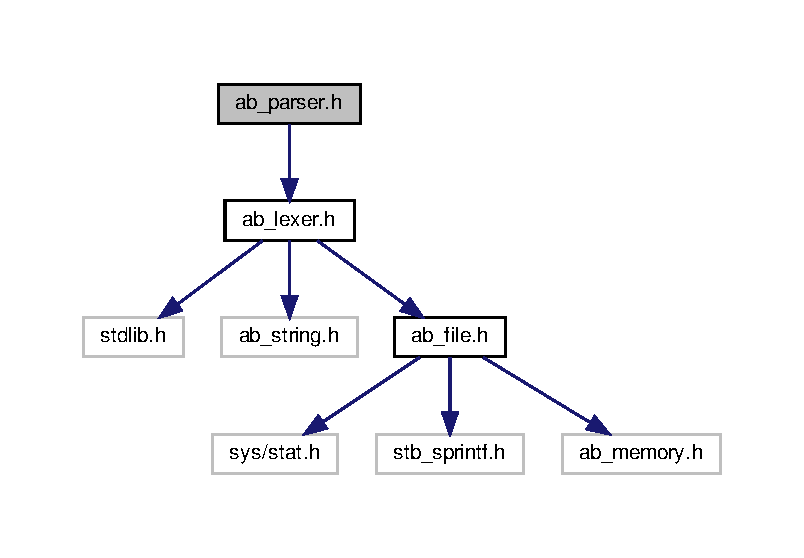
\includegraphics[width=283pt]{d5/d94/ab__parser_8h__incl}
\end{center}
\end{figure}
This graph shows which files directly or indirectly include this file\+:
\nopagebreak
\begin{figure}[H]
\begin{center}
\leavevmode
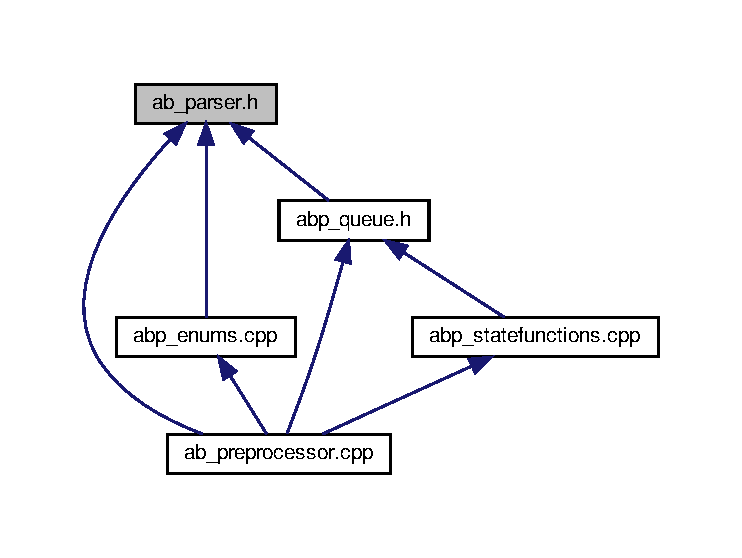
\includegraphics[width=341pt]{d9/da1/ab__parser_8h__dep__incl}
\end{center}
\end{figure}
\subsection*{Classes}
\begin{DoxyCompactItemize}
\item 
struct \hyperlink{structtag}{tag}
\item 
struct \hyperlink{structterm__typeexpr}{term\+\_\+typeexpr}
\item 
struct \hyperlink{structterm__definedfunction}{term\+\_\+definedfunction}
\item 
struct \hyperlink{structterm__statemachine}{term\+\_\+statemachine}
\item 
struct \hyperlink{structterm__structitem}{term\+\_\+structitem}
\item 
struct \hyperlink{structterm__struct}{term\+\_\+struct}
\item 
struct \hyperlink{structterm__enumitem}{term\+\_\+enumitem}
\item 
struct \hyperlink{structterm__enum}{term\+\_\+enum}
\item 
struct \hyperlink{structterm__function}{term\+\_\+function}
\item 
struct \hyperlink{structterm__statefunction}{term\+\_\+statefunction}
\item 
struct \hyperlink{structparser}{parser}
\item 
struct \hyperlink{structoutput__data}{output\+\_\+data}
\end{DoxyCompactItemize}
\subsection*{Macros}
\begin{DoxyCompactItemize}
\item 
\#define \hyperlink{ab__parser_8h_aeabe8109eddf86b30deefb9d28837243}{Init\+List}(Sentinal)
\item 
\#define \hyperlink{ab__parser_8h_a5716e375532c2d8f503025f9deb10593}{Push\+Onto\+List}(Sentinal,  New\+Item)
\item 
\#define \hyperlink{ab__parser_8h_ad6441f2fd946e5baefda8733bc8ed744}{Push\+List\+Onto\+List}(To\+Sentinal,  From\+Sentinal)
\end{DoxyCompactItemize}
\subsection*{Enumerations}
\begin{DoxyCompactItemize}
\item 
enum \hyperlink{ab__parser_8h_ac9039717ce4cccacf493ee306650a423}{custom\+\_\+type} \{ \newline
\hyperlink{ab__parser_8h_ac9039717ce4cccacf493ee306650a423a365c11b5fcf955d07d55c017767c4658}{C\+T\+\_\+\+None}, 
\hyperlink{ab__parser_8h_ac9039717ce4cccacf493ee306650a423a5d9c6244fb2275c721f1f348559f2c41}{C\+T\+\_\+\+Struct}, 
\hyperlink{ab__parser_8h_ac9039717ce4cccacf493ee306650a423a0168fb837b6dd0ef60f59281336f297e}{C\+T\+\_\+\+Union}, 
\hyperlink{ab__parser_8h_ac9039717ce4cccacf493ee306650a423a48f97ab3d4222611634d568b2b11fd9f}{C\+T\+\_\+\+Class}, 
\newline
\hyperlink{ab__parser_8h_ac9039717ce4cccacf493ee306650a423a45908c6d305646ca2e5e6395752c91d3}{C\+T\+\_\+\+Enum}
 \}
\end{DoxyCompactItemize}
\subsection*{Functions}
\begin{DoxyCompactItemize}
\item 
\hyperlink{structtag}{tag} \hyperlink{ab__parser_8h_a2087ae02cf60801129cd945b8a053a01}{Parse\+Tag} (\hyperlink{structlexer}{lexer} $\ast$Lexer, \hyperlink{structparser}{parser} $\ast$Parser)
\end{DoxyCompactItemize}


\subsection{Macro Definition Documentation}
\mbox{\Hypertarget{ab__parser_8h_aeabe8109eddf86b30deefb9d28837243}\label{ab__parser_8h_aeabe8109eddf86b30deefb9d28837243}} 
\index{ab\+\_\+parser.\+h@{ab\+\_\+parser.\+h}!Init\+List@{Init\+List}}
\index{Init\+List@{Init\+List}!ab\+\_\+parser.\+h@{ab\+\_\+parser.\+h}}
\subsubsection{\texorpdfstring{Init\+List}{InitList}}
{\footnotesize\ttfamily \#define Init\+List(\begin{DoxyParamCaption}\item[{}]{Sentinal }\end{DoxyParamCaption})}

{\bfseries Value\+:}
\begin{DoxyCode}
\{ \(\backslash\)
Sentinal.Next = &Sentinal; \(\backslash\)
Sentinal.Prev = &Sentinal; \(\backslash\)
\}
\end{DoxyCode}
\mbox{\Hypertarget{ab__parser_8h_ad6441f2fd946e5baefda8733bc8ed744}\label{ab__parser_8h_ad6441f2fd946e5baefda8733bc8ed744}} 
\index{ab\+\_\+parser.\+h@{ab\+\_\+parser.\+h}!Push\+List\+Onto\+List@{Push\+List\+Onto\+List}}
\index{Push\+List\+Onto\+List@{Push\+List\+Onto\+List}!ab\+\_\+parser.\+h@{ab\+\_\+parser.\+h}}
\subsubsection{\texorpdfstring{Push\+List\+Onto\+List}{PushListOntoList}}
{\footnotesize\ttfamily \#define Push\+List\+Onto\+List(\begin{DoxyParamCaption}\item[{}]{To\+Sentinal,  }\item[{}]{From\+Sentinal }\end{DoxyParamCaption})}

{\bfseries Value\+:}
\begin{DoxyCode}
\{ \(\backslash\)
FromSentinal.Prev->Next = &ToSentinal; \(\backslash\)
FromSentinal.Next->Prev = ToSentinal.Prev; \(\backslash\)
ToSentinal.Prev->Next = FromSentinal.Next; \(\backslash\)
ToSentinal.Prev = FromSentinal.Prev; \(\backslash\)
\}
\end{DoxyCode}
\mbox{\Hypertarget{ab__parser_8h_a5716e375532c2d8f503025f9deb10593}\label{ab__parser_8h_a5716e375532c2d8f503025f9deb10593}} 
\index{ab\+\_\+parser.\+h@{ab\+\_\+parser.\+h}!Push\+Onto\+List@{Push\+Onto\+List}}
\index{Push\+Onto\+List@{Push\+Onto\+List}!ab\+\_\+parser.\+h@{ab\+\_\+parser.\+h}}
\subsubsection{\texorpdfstring{Push\+Onto\+List}{PushOntoList}}
{\footnotesize\ttfamily \#define Push\+Onto\+List(\begin{DoxyParamCaption}\item[{}]{Sentinal,  }\item[{}]{New\+Item }\end{DoxyParamCaption})}

{\bfseries Value\+:}
\begin{DoxyCode}
\{ \(\backslash\)
NewItem->Next = &Sentinal; \(\backslash\)
NewItem->Prev = Sentinal.Prev; \(\backslash\)
Sentinal.Prev->Next = NewItem; \(\backslash\)
Sentinal.Prev = NewItem; \(\backslash\)
\}
\end{DoxyCode}


\subsection{Enumeration Type Documentation}
\mbox{\Hypertarget{ab__parser_8h_ac9039717ce4cccacf493ee306650a423}\label{ab__parser_8h_ac9039717ce4cccacf493ee306650a423}} 
\index{ab\+\_\+parser.\+h@{ab\+\_\+parser.\+h}!custom\+\_\+type@{custom\+\_\+type}}
\index{custom\+\_\+type@{custom\+\_\+type}!ab\+\_\+parser.\+h@{ab\+\_\+parser.\+h}}
\subsubsection{\texorpdfstring{custom\+\_\+type}{custom\_type}}
{\footnotesize\ttfamily enum \hyperlink{ab__parser_8h_ac9039717ce4cccacf493ee306650a423}{custom\+\_\+type}}

\begin{DoxyEnumFields}{Enumerator}
\raisebox{\heightof{T}}[0pt][0pt]{\index{C\+T\+\_\+\+None@{C\+T\+\_\+\+None}!ab\+\_\+parser.\+h@{ab\+\_\+parser.\+h}}\index{ab\+\_\+parser.\+h@{ab\+\_\+parser.\+h}!C\+T\+\_\+\+None@{C\+T\+\_\+\+None}}}\mbox{\Hypertarget{ab__parser_8h_ac9039717ce4cccacf493ee306650a423a365c11b5fcf955d07d55c017767c4658}\label{ab__parser_8h_ac9039717ce4cccacf493ee306650a423a365c11b5fcf955d07d55c017767c4658}} 
C\+T\+\_\+\+None&\\
\hline

\raisebox{\heightof{T}}[0pt][0pt]{\index{C\+T\+\_\+\+Struct@{C\+T\+\_\+\+Struct}!ab\+\_\+parser.\+h@{ab\+\_\+parser.\+h}}\index{ab\+\_\+parser.\+h@{ab\+\_\+parser.\+h}!C\+T\+\_\+\+Struct@{C\+T\+\_\+\+Struct}}}\mbox{\Hypertarget{ab__parser_8h_ac9039717ce4cccacf493ee306650a423a5d9c6244fb2275c721f1f348559f2c41}\label{ab__parser_8h_ac9039717ce4cccacf493ee306650a423a5d9c6244fb2275c721f1f348559f2c41}} 
C\+T\+\_\+\+Struct&\\
\hline

\raisebox{\heightof{T}}[0pt][0pt]{\index{C\+T\+\_\+\+Union@{C\+T\+\_\+\+Union}!ab\+\_\+parser.\+h@{ab\+\_\+parser.\+h}}\index{ab\+\_\+parser.\+h@{ab\+\_\+parser.\+h}!C\+T\+\_\+\+Union@{C\+T\+\_\+\+Union}}}\mbox{\Hypertarget{ab__parser_8h_ac9039717ce4cccacf493ee306650a423a0168fb837b6dd0ef60f59281336f297e}\label{ab__parser_8h_ac9039717ce4cccacf493ee306650a423a0168fb837b6dd0ef60f59281336f297e}} 
C\+T\+\_\+\+Union&\\
\hline

\raisebox{\heightof{T}}[0pt][0pt]{\index{C\+T\+\_\+\+Class@{C\+T\+\_\+\+Class}!ab\+\_\+parser.\+h@{ab\+\_\+parser.\+h}}\index{ab\+\_\+parser.\+h@{ab\+\_\+parser.\+h}!C\+T\+\_\+\+Class@{C\+T\+\_\+\+Class}}}\mbox{\Hypertarget{ab__parser_8h_ac9039717ce4cccacf493ee306650a423a48f97ab3d4222611634d568b2b11fd9f}\label{ab__parser_8h_ac9039717ce4cccacf493ee306650a423a48f97ab3d4222611634d568b2b11fd9f}} 
C\+T\+\_\+\+Class&\\
\hline

\raisebox{\heightof{T}}[0pt][0pt]{\index{C\+T\+\_\+\+Enum@{C\+T\+\_\+\+Enum}!ab\+\_\+parser.\+h@{ab\+\_\+parser.\+h}}\index{ab\+\_\+parser.\+h@{ab\+\_\+parser.\+h}!C\+T\+\_\+\+Enum@{C\+T\+\_\+\+Enum}}}\mbox{\Hypertarget{ab__parser_8h_ac9039717ce4cccacf493ee306650a423a45908c6d305646ca2e5e6395752c91d3}\label{ab__parser_8h_ac9039717ce4cccacf493ee306650a423a45908c6d305646ca2e5e6395752c91d3}} 
C\+T\+\_\+\+Enum&\\
\hline

\end{DoxyEnumFields}


\subsection{Function Documentation}
\mbox{\Hypertarget{ab__parser_8h_a2087ae02cf60801129cd945b8a053a01}\label{ab__parser_8h_a2087ae02cf60801129cd945b8a053a01}} 
\index{ab\+\_\+parser.\+h@{ab\+\_\+parser.\+h}!Parse\+Tag@{Parse\+Tag}}
\index{Parse\+Tag@{Parse\+Tag}!ab\+\_\+parser.\+h@{ab\+\_\+parser.\+h}}
\subsubsection{\texorpdfstring{Parse\+Tag()}{ParseTag()}}
{\footnotesize\ttfamily \hyperlink{structtag}{tag} Parse\+Tag (\begin{DoxyParamCaption}\item[{\hyperlink{structlexer}{lexer} $\ast$}]{Lexer,  }\item[{\hyperlink{structparser}{parser} $\ast$}]{Parser }\end{DoxyParamCaption})}


\hypertarget{ab__preprocessor_8cpp}{}\doxysection{ab\+\_\+preprocessor.\+cpp File Reference}
\label{ab__preprocessor_8cpp}\index{ab\_preprocessor.cpp@{ab\_preprocessor.cpp}}


A basic preprocessor to generate a header file.  


{\ttfamily \#include $<$stdio.\+h$>$}\newline
{\ttfamily \#include $<$time.\+h$>$}\newline
{\ttfamily \#include \char`\"{}ab\+\_\+common.\+h\char`\"{}}\newline
{\ttfamily \#include \char`\"{}ab\+\_\+memory.\+h\char`\"{}}\newline
{\ttfamily \#include \char`\"{}ab\+\_\+string.\+h\char`\"{}}\newline
{\ttfamily \#include \char`\"{}ab\+\_\+file.\+h\char`\"{}}\newline
{\ttfamily \#include \char`\"{}ab\+\_\+lexer.\+h\char`\"{}}\newline
{\ttfamily \#include \char`\"{}ab\+\_\+parser.\+h\char`\"{}}\newline
{\ttfamily \#include \char`\"{}stb\+\_\+sprintf.\+h\char`\"{}}\newline
{\ttfamily \#include \char`\"{}abp\+\_\+queue.\+h\char`\"{}}\newline
{\ttfamily \#include \char`\"{}abp\+\_\+enums.\+cpp\char`\"{}}\newline
{\ttfamily \#include \char`\"{}abp\+\_\+statefunctions.\+cpp\char`\"{}}\newline
{\ttfamily \#include \char`\"{}abp\+\_\+structs.\+cpp\char`\"{}}\newline
Include dependency graph for ab\+\_\+preprocessor.\+cpp\+:\nopagebreak
\begin{figure}[H]
\begin{center}
\leavevmode
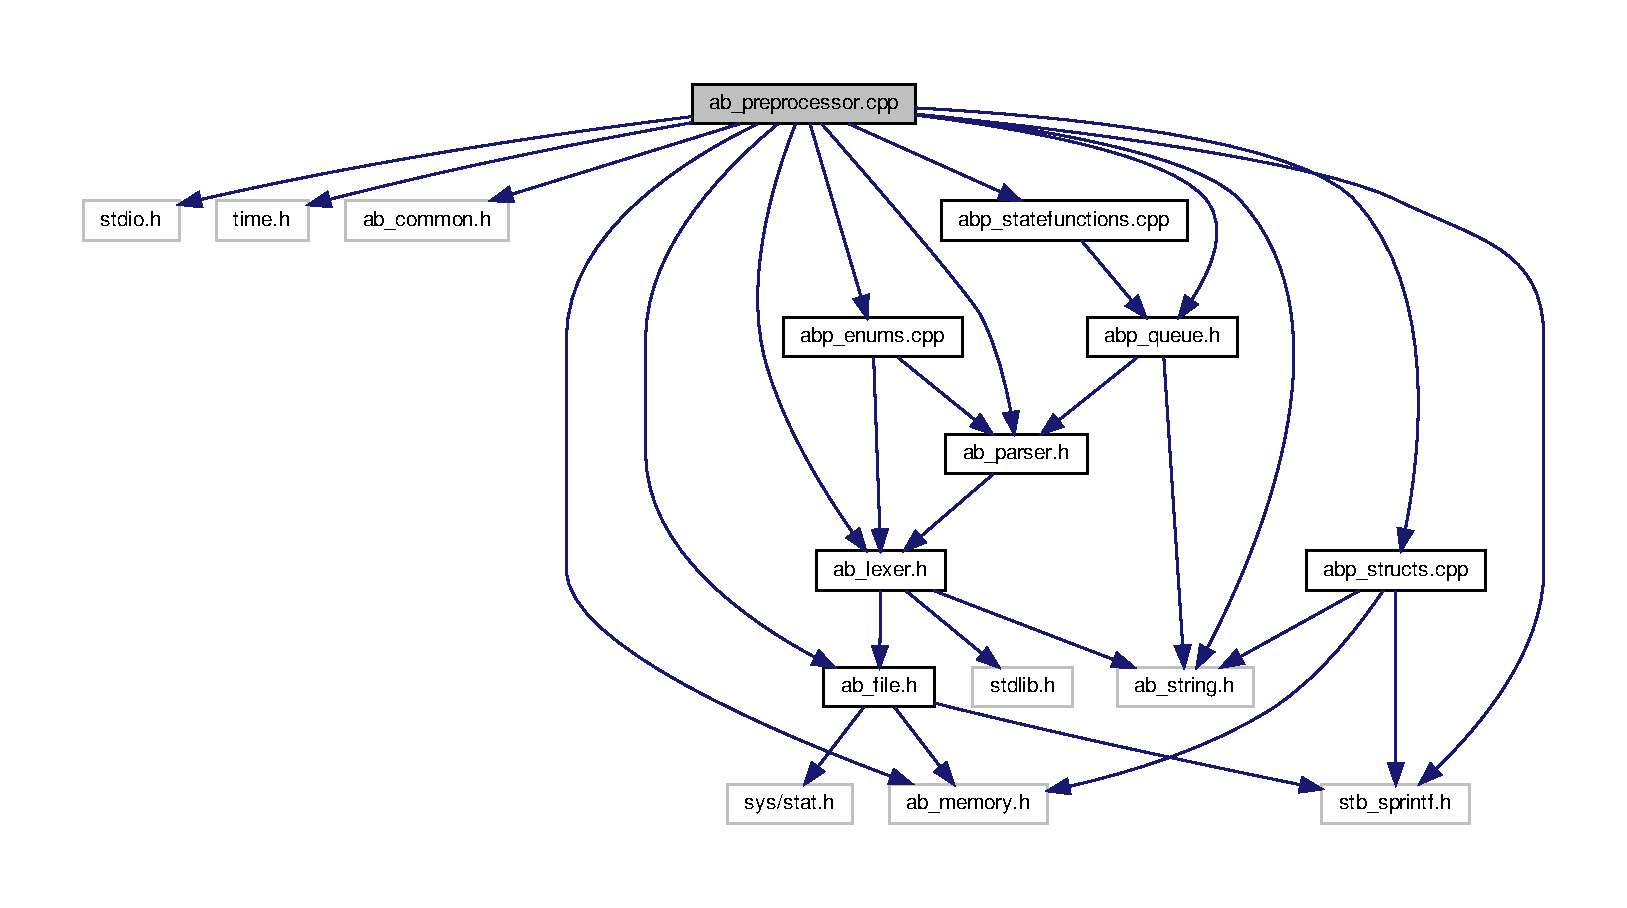
\includegraphics[width=350pt]{d5/d78/ab__preprocessor_8cpp__incl}
\end{center}
\end{figure}
\doxysubsection*{Macros}
\begin{DoxyCompactItemize}
\item 
\#define \mbox{\hyperlink{ab__preprocessor_8cpp_a1c6d5de492ac61ad29aec7aa9a436bbf}{V\+E\+R\+S\+I\+ON}}~\char`\"{}1.\+0\char`\"{}
\item 
\#define \mbox{\hyperlink{ab__preprocessor_8cpp_a912cf300a2ea45ef953fdbd09013ff2f}{M\+E\+M\+O\+R\+Y\+\_\+\+S\+RC}}
\item 
\#define \mbox{\hyperlink{ab__preprocessor_8cpp_a6bb51ed2ff4eb52256ab43148cb826aa}{S\+T\+R\+I\+N\+G\+\_\+\+S\+RC}}
\item 
\#define \mbox{\hyperlink{ab__preprocessor_8cpp_ac56ca87f735628b6d1db0d34f25978ea}{A\+B\+\_\+\+F\+I\+L\+E\+\_\+\+S\+RC}}
\item 
\#define \mbox{\hyperlink{ab__preprocessor_8cpp_a2affa792e6608b227a3545165d400000}{A\+B\+\_\+\+L\+E\+X\+E\+R\+\_\+\+S\+RC}}
\item 
\#define \mbox{\hyperlink{ab__preprocessor_8cpp_ac4d4c61013514e012213131cfef4ce1e}{A\+B\+\_\+\+P\+A\+R\+S\+E\+R\+\_\+\+S\+RC}}
\item 
\#define \mbox{\hyperlink{ab__preprocessor_8cpp_a840dcc5088daf9a542cceb05e306855c}{S\+T\+B\+\_\+\+S\+P\+R\+I\+N\+T\+F\+\_\+\+I\+M\+P\+L\+E\+M\+E\+N\+T\+A\+T\+I\+ON}}
\item 
\#define \mbox{\hyperlink{ab__preprocessor_8cpp_ab8a73ef02993098f2a7b728281f7922e}{A\+B\+P\+\_\+\+Q\+U\+E\+U\+E\+\_\+\+S\+RC}}
\end{DoxyCompactItemize}
\doxysubsection*{Functions}
\begin{DoxyCompactItemize}
\item 
void \mbox{\hyperlink{ab__preprocessor_8cpp_a1ceb4d4f9c01cff4e92adcca4d31949f}{Write\+To\+Output}} (\mbox{\hyperlink{structoutput__data}{output\+\_\+data}} $\ast$Output, memory\+\_\+arena $\ast$Memory, char const $\ast$String,...)
\item 
void \mbox{\hyperlink{ab__preprocessor_8cpp_a543263769375c19c9f59fe002d5e50ef}{Copy\+To\+Output}} (\mbox{\hyperlink{structoutput__data}{output\+\_\+data}} $\ast$Output, memory\+\_\+arena $\ast$Memory, char const $\ast$String)
\item 
void \mbox{\hyperlink{ab__preprocessor_8cpp_a8f1cafd703a8d82c50649694e22999bd}{Copy\+To\+Output}} (\mbox{\hyperlink{structoutput__data}{output\+\_\+data}} $\ast$To\+Output, memory\+\_\+arena $\ast$Memory, \mbox{\hyperlink{structoutput__data}{output\+\_\+data}} $\ast$From\+Output)
\item 
\mbox{\hyperlink{structoutput__data}{output\+\_\+data}} $\ast$ \mbox{\hyperlink{ab__preprocessor_8cpp_a3eed7463a6e214d1f4cf577811607834}{Generate\+Output}} (memory\+\_\+arena $\ast$Memory, char const $\ast$Output\+File, \mbox{\hyperlink{structoutput__data}{output\+\_\+data}} $\ast$Header\+Includes, \mbox{\hyperlink{structoutput__data}{output\+\_\+data}} $\ast$Header, \mbox{\hyperlink{structoutput__data}{output\+\_\+data}} $\ast$Definition)
\item 
void \mbox{\hyperlink{ab__preprocessor_8cpp_a64d78688e6ec9c0c314050130b29d06b}{Create\+Full\+Filename}} (char $\ast$Output, size\+\_\+t Max\+Length, char const $\ast$Path, u32 Number)
\begin{DoxyCompactList}\small\item\em Write out file. \end{DoxyCompactList}\item 
void \mbox{\hyperlink{ab__preprocessor_8cpp_a2015c745c296d4961772e6f3bb73f7be}{Write\+Output\+To\+File}} (\mbox{\hyperlink{structoutput__data}{output\+\_\+data}} $\ast$Output\+Data, char const $\ast$Source\+Directory, char const $\ast$Output\+File)
\item 
void \mbox{\hyperlink{ab__preprocessor_8cpp_aa5d09e49545215d26b1b3a7f7044f79e}{Write\+Output\+To\+Std\+Out}} (\mbox{\hyperlink{structoutput__data}{output\+\_\+data}} $\ast$Output\+Data)
\begin{DoxyCompactList}\small\item\em Write out to screen. \end{DoxyCompactList}\item 
int \mbox{\hyperlink{ab__preprocessor_8cpp_a3c04138a5bfe5d72780bb7e82a18e627}{main}} (int argc, char $\ast$$\ast$argv)
\end{DoxyCompactItemize}
\doxysubsection*{Variables}
\begin{DoxyCompactItemize}
\item 
char const  $\ast$ \mbox{\hyperlink{ab__preprocessor_8cpp_af946521958bb4da2ca5af31b7b9d67c7}{Generated\+Tag}} = \char`\"{}/$\ast$ $\ast$ G\+E\+N\+E\+R\+A\+T\+ED $\ast$ $\ast$/\char`\"{}
\end{DoxyCompactItemize}


\doxysubsection{Detailed Description}
A basic preprocessor to generate a header file. 

\begin{DoxyAuthor}{Author}
Amos Buchanan 
\end{DoxyAuthor}
\begin{DoxyVersion}{Version}
1.\+0 
\end{DoxyVersion}
\begin{DoxyDate}{Date}
2020 
\end{DoxyDate}
\begin{DoxyCopyright}{Copyright}
\href{https://opensource.org/licenses/MIT}{\texttt{ M\+IT Public License}}
\end{DoxyCopyright}
This is a basic pre-\/preprocessor that reads in the source files in a directory and outputs a generated source file with a number of standard functions. For usage, see the project \mbox{\hyperlink{Readme_8md}{Readme.\+md}} file.\hypertarget{ab__preprocessor_8cpp_autotoc_md1}{}\doxysubsection{M\+I\+T License}\label{ab__preprocessor_8cpp_autotoc_md1}
\href{https://opensource.org/licenses/MIT}{\texttt{ M\+IT Public License}}

Copyright 2020 Amos Buchanan

Permission is hereby granted, free of charge, to any person obtaining a copy of this software and associated documentation files (the \char`\"{}\+Software\char`\"{}), to deal in the Software without restriction, including without limitation the rights to use, copy, modify, merge, publish, distribute, sublicense, and/or sell copies of the Software, and to permit persons to whom the Software is furnished to do so, subject to the following conditions\+:

The above copyright notice and this permission notice shall be included in all copies or substantial portions of the Software.

T\+HE S\+O\+F\+T\+W\+A\+RE IS P\+R\+O\+V\+I\+D\+ED \char`\"{}\+A\+S I\+S\char`\"{}, W\+I\+T\+H\+O\+UT W\+A\+R\+R\+A\+N\+TY OF A\+NY K\+I\+ND, E\+X\+P\+R\+E\+SS OR I\+M\+P\+L\+I\+ED, I\+N\+C\+L\+U\+D\+I\+NG B\+UT N\+OT L\+I\+M\+I\+T\+ED TO T\+HE W\+A\+R\+R\+A\+N\+T\+I\+ES OF M\+E\+R\+C\+H\+A\+N\+T\+A\+B\+I\+L\+I\+TY, F\+I\+T\+N\+E\+SS F\+OR A P\+A\+R\+T\+I\+C\+U\+L\+AR P\+U\+R\+P\+O\+SE A\+ND N\+O\+N\+I\+N\+F\+R\+I\+N\+G\+E\+M\+E\+NT. IN NO E\+V\+E\+NT S\+H\+A\+LL T\+HE A\+U\+T\+H\+O\+RS OR C\+O\+P\+Y\+R\+I\+G\+HT H\+O\+L\+D\+E\+RS BE L\+I\+A\+B\+LE F\+OR A\+NY C\+L\+A\+IM, D\+A\+M\+A\+G\+ES OR O\+T\+H\+ER L\+I\+A\+B\+I\+L\+I\+TY, W\+H\+E\+T\+H\+ER IN AN A\+C\+T\+I\+ON OF C\+O\+N\+T\+R\+A\+CT, T\+O\+RT OR O\+T\+H\+E\+R\+W\+I\+SE, A\+R\+I\+S\+I\+NG F\+R\+OM, O\+UT OF OR IN C\+O\+N\+N\+E\+C\+T\+I\+ON W\+I\+TH T\+HE S\+O\+F\+T\+W\+A\+RE OR T\+HE U\+SE OR O\+T\+H\+ER D\+E\+A\+L\+I\+N\+GS IN T\+HE S\+O\+F\+T\+W\+A\+RE. 

\doxysubsection{Macro Definition Documentation}
\mbox{\Hypertarget{ab__preprocessor_8cpp_ac56ca87f735628b6d1db0d34f25978ea}\label{ab__preprocessor_8cpp_ac56ca87f735628b6d1db0d34f25978ea}} 
\index{ab\_preprocessor.cpp@{ab\_preprocessor.cpp}!AB\_FILE\_SRC@{AB\_FILE\_SRC}}
\index{AB\_FILE\_SRC@{AB\_FILE\_SRC}!ab\_preprocessor.cpp@{ab\_preprocessor.cpp}}
\doxysubsubsection{\texorpdfstring{AB\_FILE\_SRC}{AB\_FILE\_SRC}}
{\footnotesize\ttfamily \#define A\+B\+\_\+\+F\+I\+L\+E\+\_\+\+S\+RC}

\mbox{\Hypertarget{ab__preprocessor_8cpp_a2affa792e6608b227a3545165d400000}\label{ab__preprocessor_8cpp_a2affa792e6608b227a3545165d400000}} 
\index{ab\_preprocessor.cpp@{ab\_preprocessor.cpp}!AB\_LEXER\_SRC@{AB\_LEXER\_SRC}}
\index{AB\_LEXER\_SRC@{AB\_LEXER\_SRC}!ab\_preprocessor.cpp@{ab\_preprocessor.cpp}}
\doxysubsubsection{\texorpdfstring{AB\_LEXER\_SRC}{AB\_LEXER\_SRC}}
{\footnotesize\ttfamily \#define A\+B\+\_\+\+L\+E\+X\+E\+R\+\_\+\+S\+RC}

\mbox{\Hypertarget{ab__preprocessor_8cpp_ac4d4c61013514e012213131cfef4ce1e}\label{ab__preprocessor_8cpp_ac4d4c61013514e012213131cfef4ce1e}} 
\index{ab\_preprocessor.cpp@{ab\_preprocessor.cpp}!AB\_PARSER\_SRC@{AB\_PARSER\_SRC}}
\index{AB\_PARSER\_SRC@{AB\_PARSER\_SRC}!ab\_preprocessor.cpp@{ab\_preprocessor.cpp}}
\doxysubsubsection{\texorpdfstring{AB\_PARSER\_SRC}{AB\_PARSER\_SRC}}
{\footnotesize\ttfamily \#define A\+B\+\_\+\+P\+A\+R\+S\+E\+R\+\_\+\+S\+RC}

\mbox{\Hypertarget{ab__preprocessor_8cpp_ab8a73ef02993098f2a7b728281f7922e}\label{ab__preprocessor_8cpp_ab8a73ef02993098f2a7b728281f7922e}} 
\index{ab\_preprocessor.cpp@{ab\_preprocessor.cpp}!ABP\_QUEUE\_SRC@{ABP\_QUEUE\_SRC}}
\index{ABP\_QUEUE\_SRC@{ABP\_QUEUE\_SRC}!ab\_preprocessor.cpp@{ab\_preprocessor.cpp}}
\doxysubsubsection{\texorpdfstring{ABP\_QUEUE\_SRC}{ABP\_QUEUE\_SRC}}
{\footnotesize\ttfamily \#define A\+B\+P\+\_\+\+Q\+U\+E\+U\+E\+\_\+\+S\+RC}

\mbox{\Hypertarget{ab__preprocessor_8cpp_a912cf300a2ea45ef953fdbd09013ff2f}\label{ab__preprocessor_8cpp_a912cf300a2ea45ef953fdbd09013ff2f}} 
\index{ab\_preprocessor.cpp@{ab\_preprocessor.cpp}!MEMORY\_SRC@{MEMORY\_SRC}}
\index{MEMORY\_SRC@{MEMORY\_SRC}!ab\_preprocessor.cpp@{ab\_preprocessor.cpp}}
\doxysubsubsection{\texorpdfstring{MEMORY\_SRC}{MEMORY\_SRC}}
{\footnotesize\ttfamily \#define M\+E\+M\+O\+R\+Y\+\_\+\+S\+RC}

\mbox{\Hypertarget{ab__preprocessor_8cpp_a840dcc5088daf9a542cceb05e306855c}\label{ab__preprocessor_8cpp_a840dcc5088daf9a542cceb05e306855c}} 
\index{ab\_preprocessor.cpp@{ab\_preprocessor.cpp}!STB\_SPRINTF\_IMPLEMENTATION@{STB\_SPRINTF\_IMPLEMENTATION}}
\index{STB\_SPRINTF\_IMPLEMENTATION@{STB\_SPRINTF\_IMPLEMENTATION}!ab\_preprocessor.cpp@{ab\_preprocessor.cpp}}
\doxysubsubsection{\texorpdfstring{STB\_SPRINTF\_IMPLEMENTATION}{STB\_SPRINTF\_IMPLEMENTATION}}
{\footnotesize\ttfamily \#define S\+T\+B\+\_\+\+S\+P\+R\+I\+N\+T\+F\+\_\+\+I\+M\+P\+L\+E\+M\+E\+N\+T\+A\+T\+I\+ON}

\mbox{\Hypertarget{ab__preprocessor_8cpp_a6bb51ed2ff4eb52256ab43148cb826aa}\label{ab__preprocessor_8cpp_a6bb51ed2ff4eb52256ab43148cb826aa}} 
\index{ab\_preprocessor.cpp@{ab\_preprocessor.cpp}!STRING\_SRC@{STRING\_SRC}}
\index{STRING\_SRC@{STRING\_SRC}!ab\_preprocessor.cpp@{ab\_preprocessor.cpp}}
\doxysubsubsection{\texorpdfstring{STRING\_SRC}{STRING\_SRC}}
{\footnotesize\ttfamily \#define S\+T\+R\+I\+N\+G\+\_\+\+S\+RC}

\mbox{\Hypertarget{ab__preprocessor_8cpp_a1c6d5de492ac61ad29aec7aa9a436bbf}\label{ab__preprocessor_8cpp_a1c6d5de492ac61ad29aec7aa9a436bbf}} 
\index{ab\_preprocessor.cpp@{ab\_preprocessor.cpp}!VERSION@{VERSION}}
\index{VERSION@{VERSION}!ab\_preprocessor.cpp@{ab\_preprocessor.cpp}}
\doxysubsubsection{\texorpdfstring{VERSION}{VERSION}}
{\footnotesize\ttfamily \#define V\+E\+R\+S\+I\+ON~\char`\"{}1.\+0\char`\"{}}



\doxysubsection{Function Documentation}
\mbox{\Hypertarget{ab__preprocessor_8cpp_a543263769375c19c9f59fe002d5e50ef}\label{ab__preprocessor_8cpp_a543263769375c19c9f59fe002d5e50ef}} 
\index{ab\_preprocessor.cpp@{ab\_preprocessor.cpp}!CopyToOutput@{CopyToOutput}}
\index{CopyToOutput@{CopyToOutput}!ab\_preprocessor.cpp@{ab\_preprocessor.cpp}}
\doxysubsubsection{\texorpdfstring{CopyToOutput()}{CopyToOutput()}\hspace{0.1cm}{\footnotesize\ttfamily [1/2]}}
{\footnotesize\ttfamily void Copy\+To\+Output (\begin{DoxyParamCaption}\item[{\mbox{\hyperlink{structoutput__data}{output\+\_\+data}} $\ast$}]{Output,  }\item[{memory\+\_\+arena $\ast$}]{Memory,  }\item[{char const $\ast$}]{String }\end{DoxyParamCaption})\hspace{0.3cm}{\ttfamily [inline]}}

\mbox{\Hypertarget{ab__preprocessor_8cpp_a8f1cafd703a8d82c50649694e22999bd}\label{ab__preprocessor_8cpp_a8f1cafd703a8d82c50649694e22999bd}} 
\index{ab\_preprocessor.cpp@{ab\_preprocessor.cpp}!CopyToOutput@{CopyToOutput}}
\index{CopyToOutput@{CopyToOutput}!ab\_preprocessor.cpp@{ab\_preprocessor.cpp}}
\doxysubsubsection{\texorpdfstring{CopyToOutput()}{CopyToOutput()}\hspace{0.1cm}{\footnotesize\ttfamily [2/2]}}
{\footnotesize\ttfamily void Copy\+To\+Output (\begin{DoxyParamCaption}\item[{\mbox{\hyperlink{structoutput__data}{output\+\_\+data}} $\ast$}]{To\+Output,  }\item[{memory\+\_\+arena $\ast$}]{Memory,  }\item[{\mbox{\hyperlink{structoutput__data}{output\+\_\+data}} $\ast$}]{From\+Output }\end{DoxyParamCaption})\hspace{0.3cm}{\ttfamily [inline]}}

\mbox{\Hypertarget{ab__preprocessor_8cpp_a64d78688e6ec9c0c314050130b29d06b}\label{ab__preprocessor_8cpp_a64d78688e6ec9c0c314050130b29d06b}} 
\index{ab\_preprocessor.cpp@{ab\_preprocessor.cpp}!CreateFullFilename@{CreateFullFilename}}
\index{CreateFullFilename@{CreateFullFilename}!ab\_preprocessor.cpp@{ab\_preprocessor.cpp}}
\doxysubsubsection{\texorpdfstring{CreateFullFilename()}{CreateFullFilename()}}
{\footnotesize\ttfamily void Create\+Full\+Filename (\begin{DoxyParamCaption}\item[{char $\ast$}]{Output,  }\item[{size\+\_\+t}]{Max\+Length,  }\item[{char const $\ast$}]{Path,  }\item[{u32}]{Number }\end{DoxyParamCaption})\hspace{0.3cm}{\ttfamily [inline]}}



Write out file. 

\mbox{\Hypertarget{ab__preprocessor_8cpp_a3eed7463a6e214d1f4cf577811607834}\label{ab__preprocessor_8cpp_a3eed7463a6e214d1f4cf577811607834}} 
\index{ab\_preprocessor.cpp@{ab\_preprocessor.cpp}!GenerateOutput@{GenerateOutput}}
\index{GenerateOutput@{GenerateOutput}!ab\_preprocessor.cpp@{ab\_preprocessor.cpp}}
\doxysubsubsection{\texorpdfstring{GenerateOutput()}{GenerateOutput()}}
{\footnotesize\ttfamily \mbox{\hyperlink{structoutput__data}{output\+\_\+data}}$\ast$ Generate\+Output (\begin{DoxyParamCaption}\item[{memory\+\_\+arena $\ast$}]{Memory,  }\item[{char const $\ast$}]{Output\+File,  }\item[{\mbox{\hyperlink{structoutput__data}{output\+\_\+data}} $\ast$}]{Header\+Includes,  }\item[{\mbox{\hyperlink{structoutput__data}{output\+\_\+data}} $\ast$}]{Header,  }\item[{\mbox{\hyperlink{structoutput__data}{output\+\_\+data}} $\ast$}]{Definition }\end{DoxyParamCaption})}

\mbox{\Hypertarget{ab__preprocessor_8cpp_a3c04138a5bfe5d72780bb7e82a18e627}\label{ab__preprocessor_8cpp_a3c04138a5bfe5d72780bb7e82a18e627}} 
\index{ab\_preprocessor.cpp@{ab\_preprocessor.cpp}!main@{main}}
\index{main@{main}!ab\_preprocessor.cpp@{ab\_preprocessor.cpp}}
\doxysubsubsection{\texorpdfstring{main()}{main()}}
{\footnotesize\ttfamily int main (\begin{DoxyParamCaption}\item[{int}]{argc,  }\item[{char $\ast$$\ast$}]{argv }\end{DoxyParamCaption})}

\mbox{\Hypertarget{ab__preprocessor_8cpp_a2015c745c296d4961772e6f3bb73f7be}\label{ab__preprocessor_8cpp_a2015c745c296d4961772e6f3bb73f7be}} 
\index{ab\_preprocessor.cpp@{ab\_preprocessor.cpp}!WriteOutputToFile@{WriteOutputToFile}}
\index{WriteOutputToFile@{WriteOutputToFile}!ab\_preprocessor.cpp@{ab\_preprocessor.cpp}}
\doxysubsubsection{\texorpdfstring{WriteOutputToFile()}{WriteOutputToFile()}}
{\footnotesize\ttfamily void Write\+Output\+To\+File (\begin{DoxyParamCaption}\item[{\mbox{\hyperlink{structoutput__data}{output\+\_\+data}} $\ast$}]{Output\+Data,  }\item[{char const $\ast$}]{Source\+Directory,  }\item[{char const $\ast$}]{Output\+File }\end{DoxyParamCaption})}

\mbox{\Hypertarget{ab__preprocessor_8cpp_aa5d09e49545215d26b1b3a7f7044f79e}\label{ab__preprocessor_8cpp_aa5d09e49545215d26b1b3a7f7044f79e}} 
\index{ab\_preprocessor.cpp@{ab\_preprocessor.cpp}!WriteOutputToStdOut@{WriteOutputToStdOut}}
\index{WriteOutputToStdOut@{WriteOutputToStdOut}!ab\_preprocessor.cpp@{ab\_preprocessor.cpp}}
\doxysubsubsection{\texorpdfstring{WriteOutputToStdOut()}{WriteOutputToStdOut()}}
{\footnotesize\ttfamily void Write\+Output\+To\+Std\+Out (\begin{DoxyParamCaption}\item[{\mbox{\hyperlink{structoutput__data}{output\+\_\+data}} $\ast$}]{Output\+Data }\end{DoxyParamCaption})}



Write out to screen. 

\mbox{\Hypertarget{ab__preprocessor_8cpp_a1ceb4d4f9c01cff4e92adcca4d31949f}\label{ab__preprocessor_8cpp_a1ceb4d4f9c01cff4e92adcca4d31949f}} 
\index{ab\_preprocessor.cpp@{ab\_preprocessor.cpp}!WriteToOutput@{WriteToOutput}}
\index{WriteToOutput@{WriteToOutput}!ab\_preprocessor.cpp@{ab\_preprocessor.cpp}}
\doxysubsubsection{\texorpdfstring{WriteToOutput()}{WriteToOutput()}}
{\footnotesize\ttfamily void Write\+To\+Output (\begin{DoxyParamCaption}\item[{\mbox{\hyperlink{structoutput__data}{output\+\_\+data}} $\ast$}]{Output,  }\item[{memory\+\_\+arena $\ast$}]{Memory,  }\item[{char const $\ast$}]{String,  }\item[{}]{... }\end{DoxyParamCaption})\hspace{0.3cm}{\ttfamily [inline]}}



\doxysubsection{Variable Documentation}
\mbox{\Hypertarget{ab__preprocessor_8cpp_af946521958bb4da2ca5af31b7b9d67c7}\label{ab__preprocessor_8cpp_af946521958bb4da2ca5af31b7b9d67c7}} 
\index{ab\_preprocessor.cpp@{ab\_preprocessor.cpp}!GeneratedTag@{GeneratedTag}}
\index{GeneratedTag@{GeneratedTag}!ab\_preprocessor.cpp@{ab\_preprocessor.cpp}}
\doxysubsubsection{\texorpdfstring{GeneratedTag}{GeneratedTag}}
{\footnotesize\ttfamily char const$\ast$ Generated\+Tag = \char`\"{}/$\ast$ $\ast$ G\+E\+N\+E\+R\+A\+T\+ED $\ast$ $\ast$/\char`\"{}}


\hypertarget{abp__enums_8cpp}{}\section{abp\+\_\+enums.\+cpp File Reference}
\label{abp__enums_8cpp}\index{abp\+\_\+enums.\+cpp@{abp\+\_\+enums.\+cpp}}


Enum Class Tags.  


{\ttfamily \#include \char`\"{}ab\+\_\+parser.\+h\char`\"{}}\newline
{\ttfamily \#include \char`\"{}ab\+\_\+lexer.\+h\char`\"{}}\newline
Include dependency graph for abp\+\_\+enums.\+cpp\+:
\nopagebreak
\begin{figure}[H]
\begin{center}
\leavevmode
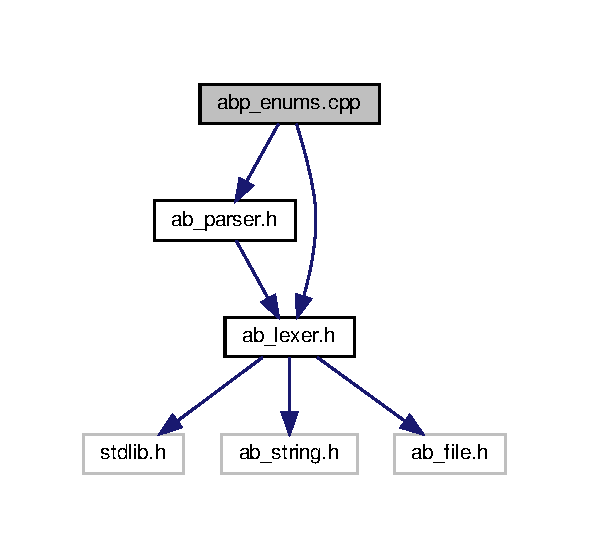
\includegraphics[width=283pt]{da/d42/abp__enums_8cpp__incl}
\end{center}
\end{figure}
This graph shows which files directly or indirectly include this file\+:
\nopagebreak
\begin{figure}[H]
\begin{center}
\leavevmode
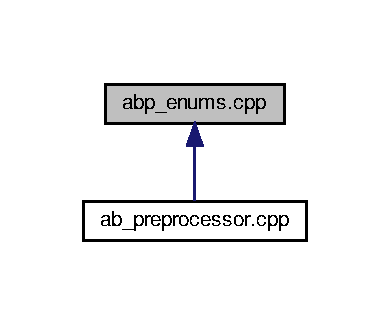
\includegraphics[width=187pt]{d9/d12/abp__enums_8cpp__dep__incl}
\end{center}
\end{figure}
\subsection*{Functions}
\begin{DoxyCompactItemize}
\item 
void \hyperlink{abp__enums_8cpp_a26413cc98eb64d610cf9f604afeb08c0}{Create\+Enum\+Json} (\hyperlink{structterm__enum}{term\+\_\+enum} $\ast$Enum, \hyperlink{structtag}{tag} $\ast$Tag, memory\+\_\+arena $\ast$Memory, \hyperlink{structoutput__data}{output\+\_\+data} $\ast$Definitions\+Out, \hyperlink{structoutput__data}{output\+\_\+data} $\ast$Functions\+Out)
\begin{DoxyCompactList}\small\item\em J\+S\+ON tag processing. \end{DoxyCompactList}\item 
void \hyperlink{abp__enums_8cpp_a4074cdfd980dd68492498531fae10c24}{Create\+Enum\+Labels} (\hyperlink{structterm__enum}{term\+\_\+enum} $\ast$Enum, \hyperlink{structtag}{tag} $\ast$Label\+Tag, memory\+\_\+arena $\ast$Memory, \hyperlink{structoutput__data}{output\+\_\+data} $\ast$Definitions\+Out, \hyperlink{structoutput__data}{output\+\_\+data} $\ast$Functions\+Out)
\begin{DoxyCompactList}\small\item\em Enum Label processing. \end{DoxyCompactList}\item 
void \hyperlink{abp__enums_8cpp_a06ef0f7fc80dcb43ccd2f3e040a30965}{Create\+Enum\+Strings} (\hyperlink{structterm__enum}{term\+\_\+enum} $\ast$Enum, \hyperlink{structtag}{tag} $\ast$Tag, memory\+\_\+arena $\ast$Memory, \hyperlink{structoutput__data}{output\+\_\+data} $\ast$Definitions\+Out, \hyperlink{structoutput__data}{output\+\_\+data} $\ast$Functions\+Out)
\begin{DoxyCompactList}\small\item\em Enum Strings T\+AG processing. \end{DoxyCompactList}\item 
void \hyperlink{abp__enums_8cpp_a9de7ea142237a33f158a301d823bfe35}{Process\+Enums} (\hyperlink{structterm__enum}{term\+\_\+enum} $\ast$Enum\+List\+Sentinal, memory\+\_\+arena $\ast$Memory, \hyperlink{structoutput__data}{output\+\_\+data} $\ast$Headers, \hyperlink{structoutput__data}{output\+\_\+data} $\ast$Definitions)
\begin{DoxyCompactList}\small\item\em Process all enums. \end{DoxyCompactList}\end{DoxyCompactItemize}


\subsection{Detailed Description}
Enum Class Tags. 

\begin{DoxyAuthor}{Author}
Amos Buchanan 
\end{DoxyAuthor}
\begin{DoxyVersion}{Version}
1.\+0 
\end{DoxyVersion}
\begin{DoxyDate}{Date}
2020 
\end{DoxyDate}
\begin{DoxyCopyright}{Copyright}
\href{https://opensource.org/licenses/MIT}{\tt M\+IT Public License}
\end{DoxyCopyright}
This is the source file for the tags used in enum class. All enum class tag definitions go here. There are no tags for C-\/style enums; any C-\/style enums with a \hyperlink{PreprocTest_8h_a2606cd56d2d8f567785bde5848176722}{T\+A\+G()} will be ignored.

See the \hyperlink{index}{Readme.md} file for more information on usage.

To add a new tag\+:
\begin{DoxyItemize}
\item Write a function to create the header and function portion of the enums.
\item Update the \hyperlink{abp__enums_8cpp_a9de7ea142237a33f158a301d823bfe35}{Process\+Enums} function with the tag and new function.
\end{DoxyItemize}\hypertarget{abp__enums_8cpp_autotoc_md1}{}\subsection{M\+I\+T License}\label{abp__enums_8cpp_autotoc_md1}
\href{https://opensource.org/licenses/MIT}{\tt https\+://opensource.\+org/licenses/\+M\+IT}

Copyright 2020 Amos Buchanan

Permission is hereby granted, free of charge, to any person obtaining a copy of this software and associated documentation files (the \char`\"{}\+Software\char`\"{}), to deal in the Software without restriction, including without limitation the rights to use, copy, modify, merge, publish, distribute, sublicense, and/or sell copies of the Software, and to permit persons to whom the Software is furnished to do so, subject to the following conditions\+:

The above copyright notice and this permission notice shall be included in all copies or substantial portions of the Software.

T\+HE S\+O\+F\+T\+W\+A\+RE IS P\+R\+O\+V\+I\+D\+ED \char`\"{}\+A\+S I\+S\char`\"{}, W\+I\+T\+H\+O\+UT W\+A\+R\+R\+A\+N\+TY OF A\+NY K\+I\+ND, E\+X\+P\+R\+E\+SS OR I\+M\+P\+L\+I\+ED, I\+N\+C\+L\+U\+D\+I\+NG B\+UT N\+OT L\+I\+M\+I\+T\+ED TO T\+HE W\+A\+R\+R\+A\+N\+T\+I\+ES OF M\+E\+R\+C\+H\+A\+N\+T\+A\+B\+I\+L\+I\+TY, F\+I\+T\+N\+E\+SS F\+OR A P\+A\+R\+T\+I\+C\+U\+L\+AR P\+U\+R\+P\+O\+SE A\+ND N\+O\+N\+I\+N\+F\+R\+I\+N\+G\+E\+M\+E\+NT. IN NO E\+V\+E\+NT S\+H\+A\+LL T\+HE A\+U\+T\+H\+O\+RS OR C\+O\+P\+Y\+R\+I\+G\+HT H\+O\+L\+D\+E\+RS BE L\+I\+A\+B\+LE F\+OR A\+NY C\+L\+A\+IM, D\+A\+M\+A\+G\+ES OR O\+T\+H\+ER L\+I\+A\+B\+I\+L\+I\+TY, W\+H\+E\+T\+H\+ER IN AN A\+C\+T\+I\+ON OF C\+O\+N\+T\+R\+A\+CT, T\+O\+RT OR O\+T\+H\+E\+R\+W\+I\+SE, A\+R\+I\+S\+I\+NG F\+R\+OM, O\+UT OF OR IN C\+O\+N\+N\+E\+C\+T\+I\+ON W\+I\+TH T\+HE S\+O\+F\+T\+W\+A\+RE OR T\+HE U\+SE OR O\+T\+H\+ER D\+E\+A\+L\+I\+N\+GS IN T\+HE S\+O\+F\+T\+W\+A\+RE. 

\subsection{Function Documentation}
\mbox{\Hypertarget{abp__enums_8cpp_a26413cc98eb64d610cf9f604afeb08c0}\label{abp__enums_8cpp_a26413cc98eb64d610cf9f604afeb08c0}} 
\index{abp\+\_\+enums.\+cpp@{abp\+\_\+enums.\+cpp}!Create\+Enum\+Json@{Create\+Enum\+Json}}
\index{Create\+Enum\+Json@{Create\+Enum\+Json}!abp\+\_\+enums.\+cpp@{abp\+\_\+enums.\+cpp}}
\subsubsection{\texorpdfstring{Create\+Enum\+Json()}{CreateEnumJson()}}
{\footnotesize\ttfamily void Create\+Enum\+Json (\begin{DoxyParamCaption}\item[{\hyperlink{structterm__enum}{term\+\_\+enum} $\ast$}]{Enum,  }\item[{\hyperlink{structtag}{tag} $\ast$}]{Tag,  }\item[{memory\+\_\+arena $\ast$}]{Memory,  }\item[{\hyperlink{structoutput__data}{output\+\_\+data} $\ast$}]{Definitions\+Out,  }\item[{\hyperlink{structoutput__data}{output\+\_\+data} $\ast$}]{Functions\+Out }\end{DoxyParamCaption})}



J\+S\+ON tag processing. 

This function processes the J\+S\+ON tag. Usage\+:


\begin{DoxyCode}
\hyperlink{PreprocTest_8h_a2606cd56d2d8f567785bde5848176722}{TAG}(JSON);
\textcolor{keyword}{enum class} SomeEnum
\{
 One,
 Two,
 Three
\};
\end{DoxyCode}
 \mbox{\Hypertarget{abp__enums_8cpp_a4074cdfd980dd68492498531fae10c24}\label{abp__enums_8cpp_a4074cdfd980dd68492498531fae10c24}} 
\index{abp\+\_\+enums.\+cpp@{abp\+\_\+enums.\+cpp}!Create\+Enum\+Labels@{Create\+Enum\+Labels}}
\index{Create\+Enum\+Labels@{Create\+Enum\+Labels}!abp\+\_\+enums.\+cpp@{abp\+\_\+enums.\+cpp}}
\subsubsection{\texorpdfstring{Create\+Enum\+Labels()}{CreateEnumLabels()}}
{\footnotesize\ttfamily void Create\+Enum\+Labels (\begin{DoxyParamCaption}\item[{\hyperlink{structterm__enum}{term\+\_\+enum} $\ast$}]{Enum,  }\item[{\hyperlink{structtag}{tag} $\ast$}]{Label\+Tag,  }\item[{memory\+\_\+arena $\ast$}]{Memory,  }\item[{\hyperlink{structoutput__data}{output\+\_\+data} $\ast$}]{Definitions\+Out,  }\item[{\hyperlink{structoutput__data}{output\+\_\+data} $\ast$}]{Functions\+Out }\end{DoxyParamCaption})}



Enum Label processing. 

This function processes enums for the Label tag.

Usage\+:


\begin{DoxyCode}
\hyperlink{PreprocTest_8h_a2606cd56d2d8f567785bde5848176722}{TAG}(Label:Number);
\textcolor{keyword}{enum class} SomeEnum
\{
\hyperlink{PreprocTest_8h_a2606cd56d2d8f567785bde5848176722}{TAG}(Number:\textcolor{stringliteral}{"1 - One"})
 One,
\hyperlink{PreprocTest_8h_a2606cd56d2d8f567785bde5848176722}{TAG}(Number:\textcolor{stringliteral}{"2 - Two"})
 Two,
\hyperlink{PreprocTest_8h_a2606cd56d2d8f567785bde5848176722}{TAG}(Number:\textcolor{stringliteral}{"3 - Three"})
 Three
\};
\end{DoxyCode}
 \mbox{\Hypertarget{abp__enums_8cpp_a06ef0f7fc80dcb43ccd2f3e040a30965}\label{abp__enums_8cpp_a06ef0f7fc80dcb43ccd2f3e040a30965}} 
\index{abp\+\_\+enums.\+cpp@{abp\+\_\+enums.\+cpp}!Create\+Enum\+Strings@{Create\+Enum\+Strings}}
\index{Create\+Enum\+Strings@{Create\+Enum\+Strings}!abp\+\_\+enums.\+cpp@{abp\+\_\+enums.\+cpp}}
\subsubsection{\texorpdfstring{Create\+Enum\+Strings()}{CreateEnumStrings()}}
{\footnotesize\ttfamily void Create\+Enum\+Strings (\begin{DoxyParamCaption}\item[{\hyperlink{structterm__enum}{term\+\_\+enum} $\ast$}]{Enum,  }\item[{\hyperlink{structtag}{tag} $\ast$}]{Tag,  }\item[{memory\+\_\+arena $\ast$}]{Memory,  }\item[{\hyperlink{structoutput__data}{output\+\_\+data} $\ast$}]{Definitions\+Out,  }\item[{\hyperlink{structoutput__data}{output\+\_\+data} $\ast$}]{Functions\+Out }\end{DoxyParamCaption})}



Enum Strings T\+AG processing. 

This function processes enums for the Strings tag.

Usage\+:


\begin{DoxyCode}
\hyperlink{PreprocTest_8h_a2606cd56d2d8f567785bde5848176722}{TAG}(Strings);
\textcolor{keyword}{enum class} SomeEnum
\{
 Unknown,
 One,
 Two,
 Three
\};
\end{DoxyCode}
 \mbox{\Hypertarget{abp__enums_8cpp_a9de7ea142237a33f158a301d823bfe35}\label{abp__enums_8cpp_a9de7ea142237a33f158a301d823bfe35}} 
\index{abp\+\_\+enums.\+cpp@{abp\+\_\+enums.\+cpp}!Process\+Enums@{Process\+Enums}}
\index{Process\+Enums@{Process\+Enums}!abp\+\_\+enums.\+cpp@{abp\+\_\+enums.\+cpp}}
\subsubsection{\texorpdfstring{Process\+Enums()}{ProcessEnums()}}
{\footnotesize\ttfamily void Process\+Enums (\begin{DoxyParamCaption}\item[{\hyperlink{structterm__enum}{term\+\_\+enum} $\ast$}]{Enum\+List\+Sentinal,  }\item[{memory\+\_\+arena $\ast$}]{Memory,  }\item[{\hyperlink{structoutput__data}{output\+\_\+data} $\ast$}]{Headers,  }\item[{\hyperlink{structoutput__data}{output\+\_\+data} $\ast$}]{Definitions }\end{DoxyParamCaption})}



Process all enums. 

Process all of the tags in the enums. This calls out to the individual functions for each tag. 
\hypertarget{abp__queue_8h}{}\doxysection{abp\+\_\+queue.\+h File Reference}
\label{abp__queue_8h}\index{abp\_queue.h@{abp\_queue.h}}
{\ttfamily \#include \char`\"{}ab\+\_\+string.\+h\char`\"{}}\newline
{\ttfamily \#include \char`\"{}ab\+\_\+parser.\+h\char`\"{}}\newline
Include dependency graph for abp\+\_\+queue.\+h\+:\nopagebreak
\begin{figure}[H]
\begin{center}
\leavevmode
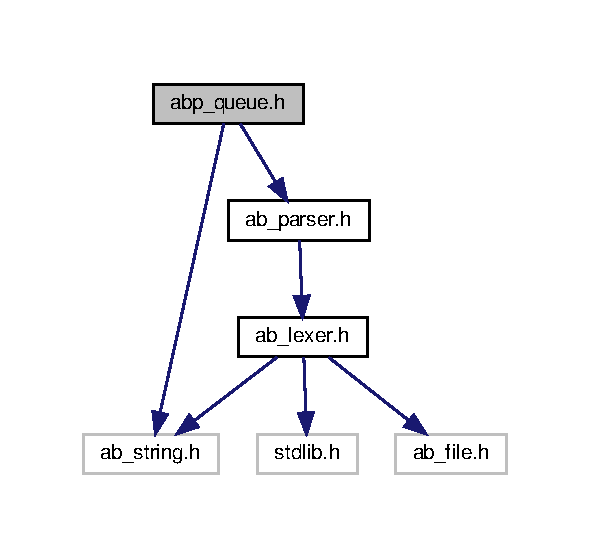
\includegraphics[width=350pt]{d6/d00/abp__queue_8h__incl}
\end{center}
\end{figure}
This graph shows which files directly or indirectly include this file\+:\nopagebreak
\begin{figure}[H]
\begin{center}
\leavevmode
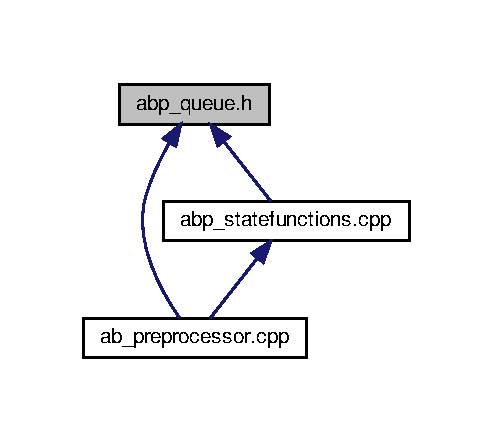
\includegraphics[width=237pt]{d6/dc7/abp__queue_8h__dep__incl}
\end{center}
\end{figure}
\doxysubsection*{Functions}
\begin{DoxyCompactItemize}
\item 
void \mbox{\hyperlink{abp__queue_8h_af0c59e83e14269261deebc96560ee1bb}{Write\+Queue\+Functions}} (abs\+\_\+stringptr Queue\+Item\+Name, u32 Queue\+Size, memory\+\_\+arena $\ast$Memory, \mbox{\hyperlink{structoutput__data}{output\+\_\+data}} $\ast$Headers, \mbox{\hyperlink{structoutput__data}{output\+\_\+data}} $\ast$Definitions)
\end{DoxyCompactItemize}


\doxysubsection{Function Documentation}
\mbox{\Hypertarget{abp__queue_8h_af0c59e83e14269261deebc96560ee1bb}\label{abp__queue_8h_af0c59e83e14269261deebc96560ee1bb}} 
\index{abp\_queue.h@{abp\_queue.h}!WriteQueueFunctions@{WriteQueueFunctions}}
\index{WriteQueueFunctions@{WriteQueueFunctions}!abp\_queue.h@{abp\_queue.h}}
\doxysubsubsection{\texorpdfstring{WriteQueueFunctions()}{WriteQueueFunctions()}}
{\footnotesize\ttfamily void Write\+Queue\+Functions (\begin{DoxyParamCaption}\item[{abs\+\_\+stringptr}]{Queue\+Item\+Name,  }\item[{u32}]{Queue\+Size,  }\item[{memory\+\_\+arena $\ast$}]{Memory,  }\item[{\mbox{\hyperlink{structoutput__data}{output\+\_\+data}} $\ast$}]{Headers,  }\item[{\mbox{\hyperlink{structoutput__data}{output\+\_\+data}} $\ast$}]{Definitions }\end{DoxyParamCaption})}


\hypertarget{abp__statefunctions_8cpp}{}\section{abp\+\_\+statefunctions.\+cpp File Reference}
\label{abp__statefunctions_8cpp}\index{abp\+\_\+statefunctions.\+cpp@{abp\+\_\+statefunctions.\+cpp}}
{\ttfamily \#include \char`\"{}abp\+\_\+queue.\+h\char`\"{}}\newline
Include dependency graph for abp\+\_\+statefunctions.\+cpp\+:\nopagebreak
\begin{figure}[H]
\begin{center}
\leavevmode
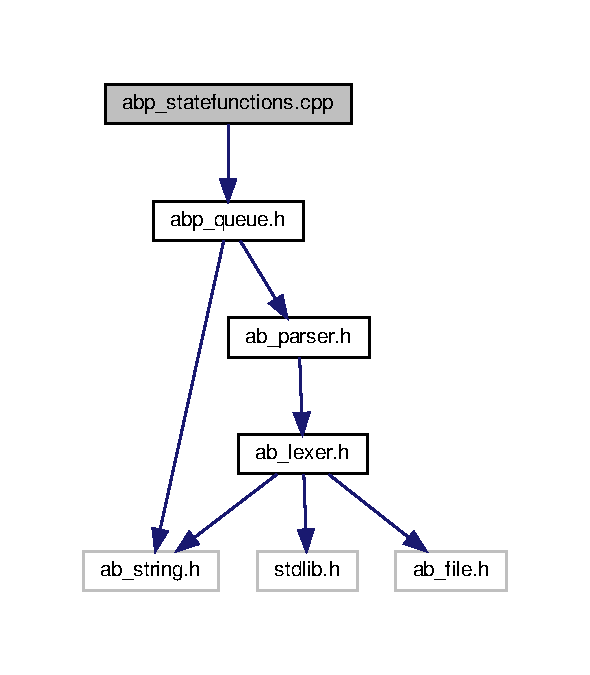
\includegraphics[width=350pt]{dc/dbe/abp__statefunctions_8cpp__incl}
\end{center}
\end{figure}
This graph shows which files directly or indirectly include this file\+:\nopagebreak
\begin{figure}[H]
\begin{center}
\leavevmode
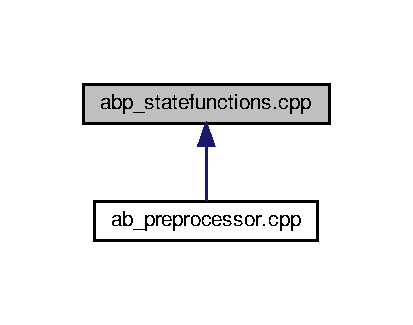
\includegraphics[width=198pt]{da/dac/abp__statefunctions_8cpp__dep__incl}
\end{center}
\end{figure}
\subsection*{Functions}
\begin{DoxyCompactItemize}
\item 
void \hyperlink{abp__statefunctions_8cpp_a26d1e099fd560e842eeb4ab5c9a39e87}{Process\+State\+Functions} (\hyperlink{structterm__statemachine}{term\+\_\+statemachine} $\ast$Machine\+List\+Sentinal, \hyperlink{structterm__definedfunction}{term\+\_\+definedfunction} $\ast$Defined\+Function\+List\+Sentinal, \hyperlink{structmemory__arena}{memory\+\_\+arena} $\ast$Memory, \hyperlink{structoutput__data}{output\+\_\+data} $\ast$Headers, \hyperlink{structoutput__data}{output\+\_\+data} $\ast$Definitions)
\end{DoxyCompactItemize}


\subsection{Function Documentation}
\mbox{\Hypertarget{abp__statefunctions_8cpp_a26d1e099fd560e842eeb4ab5c9a39e87}\label{abp__statefunctions_8cpp_a26d1e099fd560e842eeb4ab5c9a39e87}} 
\index{abp\+\_\+statefunctions.\+cpp@{abp\+\_\+statefunctions.\+cpp}!Process\+State\+Functions@{Process\+State\+Functions}}
\index{Process\+State\+Functions@{Process\+State\+Functions}!abp\+\_\+statefunctions.\+cpp@{abp\+\_\+statefunctions.\+cpp}}
\subsubsection{\texorpdfstring{Process\+State\+Functions()}{ProcessStateFunctions()}}
{\footnotesize\ttfamily void Process\+State\+Functions (\begin{DoxyParamCaption}\item[{\hyperlink{structterm__statemachine}{term\+\_\+statemachine} $\ast$}]{Machine\+List\+Sentinal,  }\item[{\hyperlink{structterm__definedfunction}{term\+\_\+definedfunction} $\ast$}]{Defined\+Function\+List\+Sentinal,  }\item[{\hyperlink{structmemory__arena}{memory\+\_\+arena} $\ast$}]{Memory,  }\item[{\hyperlink{structoutput__data}{output\+\_\+data} $\ast$}]{Headers,  }\item[{\hyperlink{structoutput__data}{output\+\_\+data} $\ast$}]{Definitions }\end{DoxyParamCaption})}


\hypertarget{abp__structs_8cpp}{}\doxysection{abp\+\_\+structs.\+cpp File Reference}
\label{abp__structs_8cpp}\index{abp\_structs.cpp@{abp\_structs.cpp}}


Struct/\+Union Class Tags.  


{\ttfamily \#include \char`\"{}ab\+\_\+string.\+h\char`\"{}}\newline
{\ttfamily \#include \char`\"{}ab\+\_\+memory.\+h\char`\"{}}\newline
{\ttfamily \#include \char`\"{}stb\+\_\+sprintf.\+h\char`\"{}}\newline
Include dependency graph for abp\+\_\+structs.\+cpp\+:\nopagebreak
\begin{figure}[H]
\begin{center}
\leavevmode
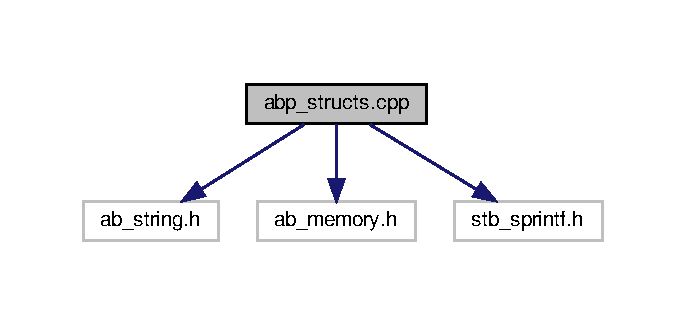
\includegraphics[width=329pt]{db/d79/abp__structs_8cpp__incl}
\end{center}
\end{figure}
This graph shows which files directly or indirectly include this file\+:\nopagebreak
\begin{figure}[H]
\begin{center}
\leavevmode
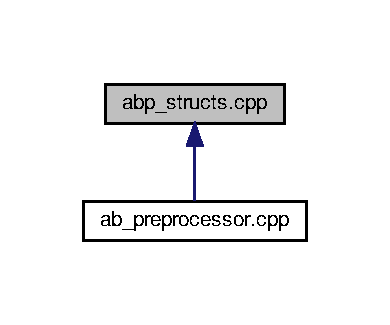
\includegraphics[width=187pt]{d8/d8f/abp__structs_8cpp__dep__incl}
\end{center}
\end{figure}
\doxysubsection*{Functions}
\begin{DoxyCompactItemize}
\item 
void \mbox{\hyperlink{abp__structs_8cpp_a9d82f4e668411580de7952f3c0089336}{Create\+Struct\+Json}} (\mbox{\hyperlink{structterm__struct}{term\+\_\+struct}} $\ast$Struct, \mbox{\hyperlink{structtag}{tag}} $\ast$Tag, memory\+\_\+arena $\ast$Memory, \mbox{\hyperlink{structoutput__data}{output\+\_\+data}} $\ast$Headers, \mbox{\hyperlink{structoutput__data}{output\+\_\+data}} $\ast$Definitions)
\begin{DoxyCompactList}\small\item\em J\+S\+ON tag processing. \end{DoxyCompactList}\item 
void \mbox{\hyperlink{abp__structs_8cpp_a0c8c66e0c511338fa2b1df03d78a52ae}{Process\+Structs}} (\mbox{\hyperlink{structterm__struct}{term\+\_\+struct}} $\ast$Struct\+List\+Sentinal, memory\+\_\+arena $\ast$Memory, \mbox{\hyperlink{structoutput__data}{output\+\_\+data}} $\ast$Headers, \mbox{\hyperlink{structoutput__data}{output\+\_\+data}} $\ast$Definitions)
\begin{DoxyCompactList}\small\item\em Handle the tags and call the struct create functions. \end{DoxyCompactList}\end{DoxyCompactItemize}


\doxysubsection{Detailed Description}
Struct/\+Union Class Tags. 

\begin{DoxyAuthor}{Author}
Amos Buchanan 
\end{DoxyAuthor}
\begin{DoxyVersion}{Version}
1.\+0 
\end{DoxyVersion}
\begin{DoxyDate}{Date}
2020 
\end{DoxyDate}
\begin{DoxyCopyright}{Copyright}
\href{https://opensource.org/licenses/MIT}{\texttt{ M\+IT Public License}}
\end{DoxyCopyright}
This is the source file for the tags used in structs and unions. All struct/union tag definitions go here. There is no difference between struct and union for this purpose.

See the \mbox{\hyperlink{index}{Readme.md}} file for more information on usage.

To add a new tag\+:
\begin{DoxyItemize}
\item Write a function to create the header and function portion of the struct functions and definitions..
\item Update the \mbox{\hyperlink{abp__structs_8cpp_a0c8c66e0c511338fa2b1df03d78a52ae}{Process\+Structs}} function with the tag and new function.
\end{DoxyItemize}\hypertarget{abp__structs_8cpp_autotoc_md4}{}\doxysubsection{M\+I\+T License}\label{abp__structs_8cpp_autotoc_md4}
\href{https://opensource.org/licenses/MIT}{\texttt{ https\+://opensource.\+org/licenses/\+M\+IT}}

Copyright 2020 Amos Buchanan

Permission is hereby granted, free of charge, to any person obtaining a copy of this software and associated documentation files (the \char`\"{}\+Software\char`\"{}), to deal in the Software without restriction, including without limitation the rights to use, copy, modify, merge, publish, distribute, sublicense, and/or sell copies of the Software, and to permit persons to whom the Software is furnished to do so, subject to the following conditions\+:

The above copyright notice and this permission notice shall be included in all copies or substantial portions of the Software.

T\+HE S\+O\+F\+T\+W\+A\+RE IS P\+R\+O\+V\+I\+D\+ED \char`\"{}\+A\+S I\+S\char`\"{}, W\+I\+T\+H\+O\+UT W\+A\+R\+R\+A\+N\+TY OF A\+NY K\+I\+ND, E\+X\+P\+R\+E\+SS OR I\+M\+P\+L\+I\+ED, I\+N\+C\+L\+U\+D\+I\+NG B\+UT N\+OT L\+I\+M\+I\+T\+ED TO T\+HE W\+A\+R\+R\+A\+N\+T\+I\+ES OF M\+E\+R\+C\+H\+A\+N\+T\+A\+B\+I\+L\+I\+TY, F\+I\+T\+N\+E\+SS F\+OR A P\+A\+R\+T\+I\+C\+U\+L\+AR P\+U\+R\+P\+O\+SE A\+ND N\+O\+N\+I\+N\+F\+R\+I\+N\+G\+E\+M\+E\+NT. IN NO E\+V\+E\+NT S\+H\+A\+LL T\+HE A\+U\+T\+H\+O\+RS OR C\+O\+P\+Y\+R\+I\+G\+HT H\+O\+L\+D\+E\+RS BE L\+I\+A\+B\+LE F\+OR A\+NY C\+L\+A\+IM, D\+A\+M\+A\+G\+ES OR O\+T\+H\+ER L\+I\+A\+B\+I\+L\+I\+TY, W\+H\+E\+T\+H\+ER IN AN A\+C\+T\+I\+ON OF C\+O\+N\+T\+R\+A\+CT, T\+O\+RT OR O\+T\+H\+E\+R\+W\+I\+SE, A\+R\+I\+S\+I\+NG F\+R\+OM, O\+UT OF OR IN C\+O\+N\+N\+E\+C\+T\+I\+ON W\+I\+TH T\+HE S\+O\+F\+T\+W\+A\+RE OR T\+HE U\+SE OR O\+T\+H\+ER D\+E\+A\+L\+I\+N\+GS IN T\+HE S\+O\+F\+T\+W\+A\+RE. 

\doxysubsection{Function Documentation}
\mbox{\Hypertarget{abp__structs_8cpp_a9d82f4e668411580de7952f3c0089336}\label{abp__structs_8cpp_a9d82f4e668411580de7952f3c0089336}} 
\index{abp\_structs.cpp@{abp\_structs.cpp}!CreateStructJson@{CreateStructJson}}
\index{CreateStructJson@{CreateStructJson}!abp\_structs.cpp@{abp\_structs.cpp}}
\doxysubsubsection{\texorpdfstring{CreateStructJson()}{CreateStructJson()}}
{\footnotesize\ttfamily void Create\+Struct\+Json (\begin{DoxyParamCaption}\item[{\mbox{\hyperlink{structterm__struct}{term\+\_\+struct}} $\ast$}]{Struct,  }\item[{\mbox{\hyperlink{structtag}{tag}} $\ast$}]{Tag,  }\item[{memory\+\_\+arena $\ast$}]{Memory,  }\item[{\mbox{\hyperlink{structoutput__data}{output\+\_\+data}} $\ast$}]{Headers,  }\item[{\mbox{\hyperlink{structoutput__data}{output\+\_\+data}} $\ast$}]{Definitions }\end{DoxyParamCaption})}



J\+S\+ON tag processing. 

Processes the J\+S\+ON tag. Usage\+:


\begin{DoxyCode}{0}
\DoxyCodeLine{\mbox{\hyperlink{PreprocTest_8h_a2606cd56d2d8f567785bde5848176722}{TAG}}(JSON);}
\DoxyCodeLine{\textcolor{keyword}{struct }SomeStruct}
\DoxyCodeLine{\{}
\DoxyCodeLine{    b8 isBoolean;}
\DoxyCodeLine{    u32 UnsignedInt;}
\DoxyCodeLine{    r32 Real32;}
\DoxyCodeLine{\};}
\end{DoxyCode}
 Object to Json Function\mbox{\Hypertarget{abp__structs_8cpp_a0c8c66e0c511338fa2b1df03d78a52ae}\label{abp__structs_8cpp_a0c8c66e0c511338fa2b1df03d78a52ae}} 
\index{abp\_structs.cpp@{abp\_structs.cpp}!ProcessStructs@{ProcessStructs}}
\index{ProcessStructs@{ProcessStructs}!abp\_structs.cpp@{abp\_structs.cpp}}
\doxysubsubsection{\texorpdfstring{ProcessStructs()}{ProcessStructs()}}
{\footnotesize\ttfamily void Process\+Structs (\begin{DoxyParamCaption}\item[{\mbox{\hyperlink{structterm__struct}{term\+\_\+struct}} $\ast$}]{Struct\+List\+Sentinal,  }\item[{memory\+\_\+arena $\ast$}]{Memory,  }\item[{\mbox{\hyperlink{structoutput__data}{output\+\_\+data}} $\ast$}]{Headers,  }\item[{\mbox{\hyperlink{structoutput__data}{output\+\_\+data}} $\ast$}]{Definitions }\end{DoxyParamCaption})}



Handle the tags and call the struct create functions. 

This is the main function for calling out to the functions that handle each tag. 
\hypertarget{Generated__Test_8h}{}\section{Generated\+\_\+\+Test.\+h File Reference}
\label{Generated__Test_8h}\index{Generated\+\_\+\+Test.\+h@{Generated\+\_\+\+Test.\+h}}
{\ttfamily \#include $<$stdlib.\+h$>$}\newline
{\ttfamily \#include \char`\"{}ab\+\_\+memory.\+h\char`\"{}}\newline
{\ttfamily \#include \char`\"{}ab\+\_\+string.\+h\char`\"{}}\newline
{\ttfamily \#include \char`\"{}stb\+\_\+sprintf.\+h\char`\"{}}\newline
{\ttfamily \#include \char`\"{}Preproc\+Test.\+h\char`\"{}}\newline
{\ttfamily \#include \char`\"{}ab\+\_\+json.\+h\char`\"{}}\newline
Include dependency graph for Generated\+\_\+\+Test.\+h\+:\nopagebreak
\begin{figure}[H]
\begin{center}
\leavevmode
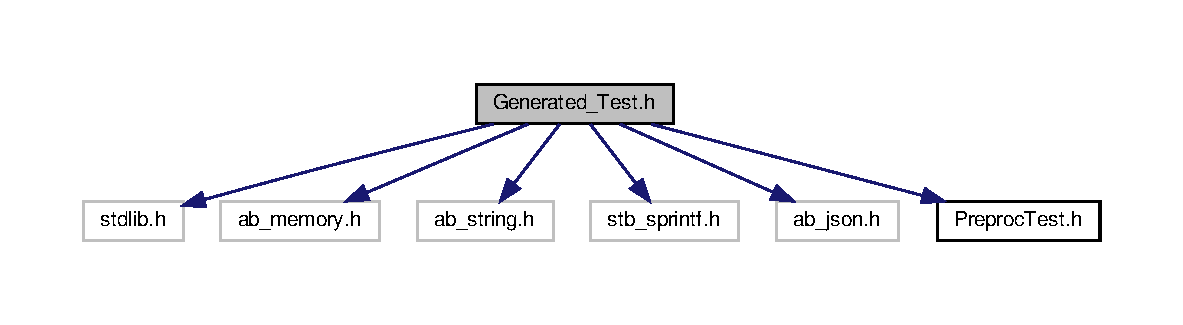
\includegraphics[width=350pt]{de/da9/Generated__Test_8h__incl}
\end{center}
\end{figure}
This graph shows which files directly or indirectly include this file\+:\nopagebreak
\begin{figure}[H]
\begin{center}
\leavevmode
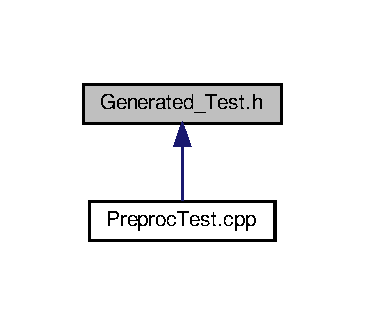
\includegraphics[width=175pt]{dd/d12/Generated__Test_8h__dep__incl}
\end{center}
\end{figure}
\subsection*{Classes}
\begin{DoxyCompactItemize}
\item 
struct \hyperlink{structtest__cmd__queue}{test\+\_\+cmd\+\_\+queue}
\item 
struct \hyperlink{structmy__json__test__existlist}{my\+\_\+json\+\_\+test\+\_\+existlist}
\end{DoxyCompactItemize}
\subsection*{Macros}
\begin{DoxyCompactItemize}
\item 
\#define \hyperlink{Generated__Test_8h_ad9b15e5b6d9b1ed55b76d9916ff6dec2}{T\+AG}(...)
\item 
\#define \hyperlink{Generated__Test_8h_ad16363f6583678566864d70afebc6a41}{S\+T\+A\+T\+E\+M\+A\+C\+H\+I\+NE}(...)
\item 
\#define \hyperlink{Generated__Test_8h_a674d40d2d82bc2df72c865d466d90a77}{\+\_\+\+G\+E\+N\+E\+R\+A\+T\+E\+D\+\_\+\+H\+E\+A\+D\+E\+R\+\_\+}
\item 
\#define \hyperlink{Generated__Test_8h_a249bf3ceb9df5c1fec7be5efe674a1ba}{\+\_\+\+A\+B\+\_\+\+G\+E\+N\+E\+R\+A\+T\+E\+D\+\_\+\+H\+E\+A\+D\+E\+R\+\_\+\+G\+E\+N\+E\+R\+A\+T\+E\+D\+\_\+\+T\+E\+S\+T\+\_\+}
\item 
\#define \hyperlink{Generated__Test_8h_a60e76ed427c4968689b9571af7254547}{T\+E\+S\+T\+\_\+\+S\+T\+A\+T\+E\+M\+A\+C\+H\+I\+NE}(name)~void name(\hyperlink{structtest__type}{test\+\_\+type} $\ast$State, \hyperlink{PreprocTest_8h_a55ed691059222a58555cf9992ec14431}{test\+\_\+cmd} Cmd, int Int, char const $\ast$String)
\end{DoxyCompactItemize}
\subsection*{Functions}
\begin{DoxyCompactItemize}
\item 
{\footnotesize template$<$typename T $>$ }\\auto \hyperlink{Generated__Test_8h_a9a60bb3cdfd4c044939d80c8e1edd6dd}{String\+To\+Enum} (const char $\ast$String) -\/$>$ T
\item 
{\footnotesize template$<$typename T $>$ }\\auto \hyperlink{Generated__Test_8h_ac56b1acaa9bd587f623d2983f921ad50}{String\+To\+Enum} (\hyperlink{structabs__stringptr}{abs\+\_\+stringptr} String) -\/$>$ T
\item 
void \hyperlink{Generated__Test_8h_a43822849924e4365ec1ad146736a7967}{Initialize\+Queue} (\hyperlink{structtest__cmd__queue}{test\+\_\+cmd\+\_\+queue} $\ast$Queue)
\item 
\hyperlink{ab__common_8h_a70e369648385b50f2d0588e8e8745275}{b8} \hyperlink{Generated__Test_8h_a24b3c990497a61d0d6aca57105e2c86a}{is\+Queue\+Empty} (\hyperlink{structtest__cmd__queue}{test\+\_\+cmd\+\_\+queue} $\ast$Queue)
\item 
\hyperlink{ab__common_8h_a70e369648385b50f2d0588e8e8745275}{b8} \hyperlink{Generated__Test_8h_a5074b01af8cb1f2124b7d04399a48c82}{is\+Queue\+Full} (\hyperlink{structtest__cmd__queue}{test\+\_\+cmd\+\_\+queue} $\ast$Queue)
\item 
\hyperlink{ab__common_8h_a70e369648385b50f2d0588e8e8745275}{b8} \hyperlink{Generated__Test_8h_a9ca011b44b1d493d71b8414f84af2f69}{Enqueue\+Command} (\hyperlink{structtest__cmd__queue}{test\+\_\+cmd\+\_\+queue} $\ast$Queue, \hyperlink{PreprocTest_8h_a55ed691059222a58555cf9992ec14431}{test\+\_\+cmd} Cmd)
\item 
\hyperlink{PreprocTest_8h_a55ed691059222a58555cf9992ec14431}{test\+\_\+cmd} \hyperlink{Generated__Test_8h_aa15eaba01fecffd4380ff2f1b4018a3a}{Dequeue\+Command} (\hyperlink{structtest__cmd__queue}{test\+\_\+cmd\+\_\+queue} $\ast$Queue)
\item 
typedef \hyperlink{Generated__Test_8h_a5b28cc9825a80c7d578bce92d5152de4}{T\+E\+S\+T\+\_\+\+S\+T\+A\+T\+E\+M\+A\+C\+H\+I\+NE} (test\+\_\+statemachine)
\item 
\hyperlink{ab__common_8h_a70e369648385b50f2d0588e8e8745275}{b8} \hyperlink{Generated__Test_8h_ad4b73e92f4af2b501841ce35b274f71c}{Go\+To\+State} (\hyperlink{structtest__type}{test\+\_\+type} $\ast$State, test\+\_\+statemachine $\ast$New\+State)
\item 
char const  $\ast$ \hyperlink{Generated__Test_8h_a36c15d4c27a71b37003bfc22b75964be}{Get\+State\+Name} (test\+\_\+statemachine $\ast$State\+Name)
\item 
\hyperlink{ab__common_8h_a70e369648385b50f2d0588e8e8745275}{b8} \hyperlink{Generated__Test_8h_aacf77a00c47b027a4331328a1071854c}{Enqueue\+Command} (\hyperlink{structtest__type}{test\+\_\+type} $\ast$State, \hyperlink{PreprocTest_8h_a55ed691059222a58555cf9992ec14431}{test\+\_\+cmd} Cmd)
\item 
\hyperlink{PreprocTest_8h_a55ed691059222a58555cf9992ec14431}{test\+\_\+cmd} \hyperlink{Generated__Test_8h_aa431f033dae8e03ce9f9e76c5897d077}{Dequeue\+Command} (\hyperlink{structtest__type}{test\+\_\+type} $\ast$State)
\item 
\hyperlink{Generated__Test_8h_ab6c57dcff4bca075ce03bbe119d0b4dd}{T\+E\+S\+T\+\_\+\+S\+T\+A\+T\+E\+M\+A\+C\+H\+I\+NE} (Idle)
\item 
\hyperlink{Generated__Test_8h_aed31da543c10eab9ca01e8b7f1e299cd}{T\+E\+S\+T\+\_\+\+S\+T\+A\+T\+E\+M\+A\+C\+H\+I\+NE} (Running)
\item 
{\footnotesize template$<$$>$ }\\auto \hyperlink{Generated__Test_8h_a3918139d94601cfee23f622cd557582f}{String\+To\+Enum$<$ test\+\_\+cmd $>$} (const char $\ast$String) -\/$>$ \hyperlink{PreprocTest_8h_a55ed691059222a58555cf9992ec14431}{test\+\_\+cmd}
\item 
{\footnotesize template$<$$>$ }\\auto \hyperlink{Generated__Test_8h_a196b200d9f8e70d10669c8841f0ece91}{String\+To\+Enum$<$ test\+\_\+cmd $>$} (\hyperlink{structabs__stringptr}{abs\+\_\+stringptr} String) -\/$>$ \hyperlink{PreprocTest_8h_a55ed691059222a58555cf9992ec14431}{test\+\_\+cmd}
\item 
constexpr \hyperlink{structabs__stringptr}{abs\+\_\+stringptr} \hyperlink{Generated__Test_8h_a6087c1644a941337a7e8ac43157a30b3}{Enum\+To\+String} (\hyperlink{PreprocTest_8h_a55ed691059222a58555cf9992ec14431}{test\+\_\+cmd} Enum\+Token)
\item 
constexpr char const  $\ast$ \hyperlink{Generated__Test_8h_a37220bfe6977f9507cffa3283af7f09b}{Enum\+To\+C\+String} (\hyperlink{PreprocTest_8h_a55ed691059222a58555cf9992ec14431}{test\+\_\+cmd} Enum\+Token)
\item 
{\footnotesize template$<$$>$ }\\auto \hyperlink{Generated__Test_8h_ad369bcb4826dc155da6b130a0fa97d13}{String\+To\+Enum$<$ en\+Colours $>$} (const char $\ast$String) -\/$>$ \hyperlink{PreprocTest_8h_a081cf1a0e70d6e2bd48c98f457742877}{en\+Colours}
\item 
{\footnotesize template$<$$>$ }\\auto \hyperlink{Generated__Test_8h_a768f3f6a292bf1dee6bd92fc1f0648e9}{String\+To\+Enum$<$ en\+Colours $>$} (\hyperlink{structabs__stringptr}{abs\+\_\+stringptr} String) -\/$>$ \hyperlink{PreprocTest_8h_a081cf1a0e70d6e2bd48c98f457742877}{en\+Colours}
\item 
constexpr \hyperlink{structabs__stringptr}{abs\+\_\+stringptr} \hyperlink{Generated__Test_8h_af1c959d0e9481a0fb8345289c1ef463a}{Enum\+To\+String} (\hyperlink{PreprocTest_8h_a081cf1a0e70d6e2bd48c98f457742877}{en\+Colours} Enum\+Token)
\item 
constexpr char const  $\ast$ \hyperlink{Generated__Test_8h_ac94b257fa3ae7dabdbdc07db0ac072c4}{Enum\+To\+C\+String} (\hyperlink{PreprocTest_8h_a081cf1a0e70d6e2bd48c98f457742877}{en\+Colours} Enum\+Token)
\item 
const char $\ast$ \hyperlink{Generated__Test_8h_a9b8638e967a81b3c211b77df49d85034}{Enum\+To\+Label\+\_\+\+Object} (\hyperlink{PreprocTest_8h_a081cf1a0e70d6e2bd48c98f457742877}{en\+Colours} Enum\+Token)
\end{DoxyCompactItemize}
\subsection*{Variables}
\begin{DoxyCompactItemize}
\item 
struct \hyperlink{structtest__cmd__queue}{test\+\_\+cmd\+\_\+queue} \hyperlink{Generated__Test_8h_a3ee2f2be736dcd0ff7e75d6ff8d2e6d5}{Initialize\+Queue}
\item 
const \hyperlink{ab__common_8h_afaa62991928fb9fb18ff0db62a040aba}{u32} \hyperlink{Generated__Test_8h_a1d64dbc5eb5071c30cc178bb11db36f7}{test\+\_\+cmd\+\_\+\+Count} = 6
\item 
const \hyperlink{ab__common_8h_afaa62991928fb9fb18ff0db62a040aba}{u32} \hyperlink{Generated__Test_8h_abd85a89ac29df78a4d1b078c54016c79}{en\+Colours\+\_\+\+Count} = 3
\end{DoxyCompactItemize}


\subsection{Macro Definition Documentation}
\mbox{\Hypertarget{Generated__Test_8h_a249bf3ceb9df5c1fec7be5efe674a1ba}\label{Generated__Test_8h_a249bf3ceb9df5c1fec7be5efe674a1ba}} 
\index{Generated\+\_\+\+Test.\+h@{Generated\+\_\+\+Test.\+h}!\+\_\+\+A\+B\+\_\+\+G\+E\+N\+E\+R\+A\+T\+E\+D\+\_\+\+H\+E\+A\+D\+E\+R\+\_\+\+G\+E\+N\+E\+R\+A\+T\+E\+D\+\_\+\+T\+E\+S\+T\+\_\+@{\+\_\+\+A\+B\+\_\+\+G\+E\+N\+E\+R\+A\+T\+E\+D\+\_\+\+H\+E\+A\+D\+E\+R\+\_\+\+G\+E\+N\+E\+R\+A\+T\+E\+D\+\_\+\+T\+E\+S\+T\+\_\+}}
\index{\+\_\+\+A\+B\+\_\+\+G\+E\+N\+E\+R\+A\+T\+E\+D\+\_\+\+H\+E\+A\+D\+E\+R\+\_\+\+G\+E\+N\+E\+R\+A\+T\+E\+D\+\_\+\+T\+E\+S\+T\+\_\+@{\+\_\+\+A\+B\+\_\+\+G\+E\+N\+E\+R\+A\+T\+E\+D\+\_\+\+H\+E\+A\+D\+E\+R\+\_\+\+G\+E\+N\+E\+R\+A\+T\+E\+D\+\_\+\+T\+E\+S\+T\+\_\+}!Generated\+\_\+\+Test.\+h@{Generated\+\_\+\+Test.\+h}}
\subsubsection{\texorpdfstring{\+\_\+\+A\+B\+\_\+\+G\+E\+N\+E\+R\+A\+T\+E\+D\+\_\+\+H\+E\+A\+D\+E\+R\+\_\+\+G\+E\+N\+E\+R\+A\+T\+E\+D\+\_\+\+T\+E\+S\+T\+\_\+}{\_AB\_GENERATED\_HEADER\_GENERATED\_TEST\_}}
{\footnotesize\ttfamily \#define \+\_\+\+A\+B\+\_\+\+G\+E\+N\+E\+R\+A\+T\+E\+D\+\_\+\+H\+E\+A\+D\+E\+R\+\_\+\+G\+E\+N\+E\+R\+A\+T\+E\+D\+\_\+\+T\+E\+S\+T\+\_\+}

\mbox{\Hypertarget{Generated__Test_8h_a674d40d2d82bc2df72c865d466d90a77}\label{Generated__Test_8h_a674d40d2d82bc2df72c865d466d90a77}} 
\index{Generated\+\_\+\+Test.\+h@{Generated\+\_\+\+Test.\+h}!\+\_\+\+G\+E\+N\+E\+R\+A\+T\+E\+D\+\_\+\+H\+E\+A\+D\+E\+R\+\_\+@{\+\_\+\+G\+E\+N\+E\+R\+A\+T\+E\+D\+\_\+\+H\+E\+A\+D\+E\+R\+\_\+}}
\index{\+\_\+\+G\+E\+N\+E\+R\+A\+T\+E\+D\+\_\+\+H\+E\+A\+D\+E\+R\+\_\+@{\+\_\+\+G\+E\+N\+E\+R\+A\+T\+E\+D\+\_\+\+H\+E\+A\+D\+E\+R\+\_\+}!Generated\+\_\+\+Test.\+h@{Generated\+\_\+\+Test.\+h}}
\subsubsection{\texorpdfstring{\+\_\+\+G\+E\+N\+E\+R\+A\+T\+E\+D\+\_\+\+H\+E\+A\+D\+E\+R\+\_\+}{\_GENERATED\_HEADER\_}}
{\footnotesize\ttfamily \#define \+\_\+\+G\+E\+N\+E\+R\+A\+T\+E\+D\+\_\+\+H\+E\+A\+D\+E\+R\+\_\+}

\mbox{\Hypertarget{Generated__Test_8h_ad16363f6583678566864d70afebc6a41}\label{Generated__Test_8h_ad16363f6583678566864d70afebc6a41}} 
\index{Generated\+\_\+\+Test.\+h@{Generated\+\_\+\+Test.\+h}!S\+T\+A\+T\+E\+M\+A\+C\+H\+I\+NE@{S\+T\+A\+T\+E\+M\+A\+C\+H\+I\+NE}}
\index{S\+T\+A\+T\+E\+M\+A\+C\+H\+I\+NE@{S\+T\+A\+T\+E\+M\+A\+C\+H\+I\+NE}!Generated\+\_\+\+Test.\+h@{Generated\+\_\+\+Test.\+h}}
\subsubsection{\texorpdfstring{S\+T\+A\+T\+E\+M\+A\+C\+H\+I\+NE}{STATEMACHINE}}
{\footnotesize\ttfamily \#define S\+T\+A\+T\+E\+M\+A\+C\+H\+I\+NE(\begin{DoxyParamCaption}\item[{}]{... }\end{DoxyParamCaption})}

\mbox{\Hypertarget{Generated__Test_8h_ad9b15e5b6d9b1ed55b76d9916ff6dec2}\label{Generated__Test_8h_ad9b15e5b6d9b1ed55b76d9916ff6dec2}} 
\index{Generated\+\_\+\+Test.\+h@{Generated\+\_\+\+Test.\+h}!T\+AG@{T\+AG}}
\index{T\+AG@{T\+AG}!Generated\+\_\+\+Test.\+h@{Generated\+\_\+\+Test.\+h}}
\subsubsection{\texorpdfstring{T\+AG}{TAG}}
{\footnotesize\ttfamily \#define T\+AG(\begin{DoxyParamCaption}\item[{}]{... }\end{DoxyParamCaption})}

G\+E\+N\+E\+R\+A\+T\+ED Code Generator Version\+: 1.\+0

This file was autogenerated. Do not edit directly, your changes will get over-\/written. This is a single file include. To include the source, add

\#define G\+E\+N\+E\+R\+A\+T\+E\+D\+\_\+\+T\+E\+S\+T\+\_\+\+S\+RC \begin{DoxyVerb}before including this this file.

If you are using JSON parsing, add 
\end{DoxyVerb}


\#define G\+E\+N\+\_\+\+J\+S\+M\+N\+\_\+\+H\+E\+A\+D\+ER \begin{DoxyVerb}Ensure the jsmn.h header is in your include directory.\end{DoxyVerb}
 \mbox{\Hypertarget{Generated__Test_8h_a60e76ed427c4968689b9571af7254547}\label{Generated__Test_8h_a60e76ed427c4968689b9571af7254547}} 
\index{Generated\+\_\+\+Test.\+h@{Generated\+\_\+\+Test.\+h}!T\+E\+S\+T\+\_\+\+S\+T\+A\+T\+E\+M\+A\+C\+H\+I\+NE@{T\+E\+S\+T\+\_\+\+S\+T\+A\+T\+E\+M\+A\+C\+H\+I\+NE}}
\index{T\+E\+S\+T\+\_\+\+S\+T\+A\+T\+E\+M\+A\+C\+H\+I\+NE@{T\+E\+S\+T\+\_\+\+S\+T\+A\+T\+E\+M\+A\+C\+H\+I\+NE}!Generated\+\_\+\+Test.\+h@{Generated\+\_\+\+Test.\+h}}
\subsubsection{\texorpdfstring{T\+E\+S\+T\+\_\+\+S\+T\+A\+T\+E\+M\+A\+C\+H\+I\+NE}{TEST\_STATEMACHINE}}
{\footnotesize\ttfamily \#define T\+E\+S\+T\+\_\+\+S\+T\+A\+T\+E\+M\+A\+C\+H\+I\+NE(\begin{DoxyParamCaption}\item[{}]{name }\end{DoxyParamCaption})~void name(\hyperlink{structtest__type}{test\+\_\+type} $\ast$State, \hyperlink{PreprocTest_8h_a55ed691059222a58555cf9992ec14431}{test\+\_\+cmd} Cmd, int Int, char const $\ast$String)}



\subsection{Function Documentation}
\mbox{\Hypertarget{Generated__Test_8h_aa15eaba01fecffd4380ff2f1b4018a3a}\label{Generated__Test_8h_aa15eaba01fecffd4380ff2f1b4018a3a}} 
\index{Generated\+\_\+\+Test.\+h@{Generated\+\_\+\+Test.\+h}!Dequeue\+Command@{Dequeue\+Command}}
\index{Dequeue\+Command@{Dequeue\+Command}!Generated\+\_\+\+Test.\+h@{Generated\+\_\+\+Test.\+h}}
\subsubsection{\texorpdfstring{Dequeue\+Command()}{DequeueCommand()}\hspace{0.1cm}{\footnotesize\ttfamily [1/2]}}
{\footnotesize\ttfamily \hyperlink{PreprocTest_8h_a55ed691059222a58555cf9992ec14431}{test\+\_\+cmd} Dequeue\+Command (\begin{DoxyParamCaption}\item[{\hyperlink{structtest__cmd__queue}{test\+\_\+cmd\+\_\+queue} $\ast$}]{Queue }\end{DoxyParamCaption})}

\mbox{\Hypertarget{Generated__Test_8h_aa431f033dae8e03ce9f9e76c5897d077}\label{Generated__Test_8h_aa431f033dae8e03ce9f9e76c5897d077}} 
\index{Generated\+\_\+\+Test.\+h@{Generated\+\_\+\+Test.\+h}!Dequeue\+Command@{Dequeue\+Command}}
\index{Dequeue\+Command@{Dequeue\+Command}!Generated\+\_\+\+Test.\+h@{Generated\+\_\+\+Test.\+h}}
\subsubsection{\texorpdfstring{Dequeue\+Command()}{DequeueCommand()}\hspace{0.1cm}{\footnotesize\ttfamily [2/2]}}
{\footnotesize\ttfamily \hyperlink{PreprocTest_8h_a55ed691059222a58555cf9992ec14431}{test\+\_\+cmd} Dequeue\+Command (\begin{DoxyParamCaption}\item[{\hyperlink{structtest__type}{test\+\_\+type} $\ast$}]{State }\end{DoxyParamCaption})}

\mbox{\Hypertarget{Generated__Test_8h_a9ca011b44b1d493d71b8414f84af2f69}\label{Generated__Test_8h_a9ca011b44b1d493d71b8414f84af2f69}} 
\index{Generated\+\_\+\+Test.\+h@{Generated\+\_\+\+Test.\+h}!Enqueue\+Command@{Enqueue\+Command}}
\index{Enqueue\+Command@{Enqueue\+Command}!Generated\+\_\+\+Test.\+h@{Generated\+\_\+\+Test.\+h}}
\subsubsection{\texorpdfstring{Enqueue\+Command()}{EnqueueCommand()}\hspace{0.1cm}{\footnotesize\ttfamily [1/2]}}
{\footnotesize\ttfamily \hyperlink{ab__common_8h_a70e369648385b50f2d0588e8e8745275}{b8} Enqueue\+Command (\begin{DoxyParamCaption}\item[{\hyperlink{structtest__cmd__queue}{test\+\_\+cmd\+\_\+queue} $\ast$}]{Queue,  }\item[{\hyperlink{PreprocTest_8h_a55ed691059222a58555cf9992ec14431}{test\+\_\+cmd}}]{Cmd }\end{DoxyParamCaption})}

\mbox{\Hypertarget{Generated__Test_8h_aacf77a00c47b027a4331328a1071854c}\label{Generated__Test_8h_aacf77a00c47b027a4331328a1071854c}} 
\index{Generated\+\_\+\+Test.\+h@{Generated\+\_\+\+Test.\+h}!Enqueue\+Command@{Enqueue\+Command}}
\index{Enqueue\+Command@{Enqueue\+Command}!Generated\+\_\+\+Test.\+h@{Generated\+\_\+\+Test.\+h}}
\subsubsection{\texorpdfstring{Enqueue\+Command()}{EnqueueCommand()}\hspace{0.1cm}{\footnotesize\ttfamily [2/2]}}
{\footnotesize\ttfamily \hyperlink{ab__common_8h_a70e369648385b50f2d0588e8e8745275}{b8} Enqueue\+Command (\begin{DoxyParamCaption}\item[{\hyperlink{structtest__type}{test\+\_\+type} $\ast$}]{State,  }\item[{\hyperlink{PreprocTest_8h_a55ed691059222a58555cf9992ec14431}{test\+\_\+cmd}}]{Cmd }\end{DoxyParamCaption})}

\mbox{\Hypertarget{Generated__Test_8h_a37220bfe6977f9507cffa3283af7f09b}\label{Generated__Test_8h_a37220bfe6977f9507cffa3283af7f09b}} 
\index{Generated\+\_\+\+Test.\+h@{Generated\+\_\+\+Test.\+h}!Enum\+To\+C\+String@{Enum\+To\+C\+String}}
\index{Enum\+To\+C\+String@{Enum\+To\+C\+String}!Generated\+\_\+\+Test.\+h@{Generated\+\_\+\+Test.\+h}}
\subsubsection{\texorpdfstring{Enum\+To\+C\+String()}{EnumToCString()}\hspace{0.1cm}{\footnotesize\ttfamily [1/2]}}
{\footnotesize\ttfamily constexpr char const$\ast$ Enum\+To\+C\+String (\begin{DoxyParamCaption}\item[{\hyperlink{PreprocTest_8h_a55ed691059222a58555cf9992ec14431}{test\+\_\+cmd}}]{Enum\+Token }\end{DoxyParamCaption})}

\mbox{\Hypertarget{Generated__Test_8h_ac94b257fa3ae7dabdbdc07db0ac072c4}\label{Generated__Test_8h_ac94b257fa3ae7dabdbdc07db0ac072c4}} 
\index{Generated\+\_\+\+Test.\+h@{Generated\+\_\+\+Test.\+h}!Enum\+To\+C\+String@{Enum\+To\+C\+String}}
\index{Enum\+To\+C\+String@{Enum\+To\+C\+String}!Generated\+\_\+\+Test.\+h@{Generated\+\_\+\+Test.\+h}}
\subsubsection{\texorpdfstring{Enum\+To\+C\+String()}{EnumToCString()}\hspace{0.1cm}{\footnotesize\ttfamily [2/2]}}
{\footnotesize\ttfamily constexpr char const$\ast$ Enum\+To\+C\+String (\begin{DoxyParamCaption}\item[{\hyperlink{PreprocTest_8h_a081cf1a0e70d6e2bd48c98f457742877}{en\+Colours}}]{Enum\+Token }\end{DoxyParamCaption})}

\mbox{\Hypertarget{Generated__Test_8h_a9b8638e967a81b3c211b77df49d85034}\label{Generated__Test_8h_a9b8638e967a81b3c211b77df49d85034}} 
\index{Generated\+\_\+\+Test.\+h@{Generated\+\_\+\+Test.\+h}!Enum\+To\+Label\+\_\+\+Object@{Enum\+To\+Label\+\_\+\+Object}}
\index{Enum\+To\+Label\+\_\+\+Object@{Enum\+To\+Label\+\_\+\+Object}!Generated\+\_\+\+Test.\+h@{Generated\+\_\+\+Test.\+h}}
\subsubsection{\texorpdfstring{Enum\+To\+Label\+\_\+\+Object()}{EnumToLabel\_Object()}}
{\footnotesize\ttfamily const char$\ast$ Enum\+To\+Label\+\_\+\+Object (\begin{DoxyParamCaption}\item[{\hyperlink{PreprocTest_8h_a081cf1a0e70d6e2bd48c98f457742877}{en\+Colours}}]{Enum\+Token }\end{DoxyParamCaption})}

\mbox{\Hypertarget{Generated__Test_8h_a6087c1644a941337a7e8ac43157a30b3}\label{Generated__Test_8h_a6087c1644a941337a7e8ac43157a30b3}} 
\index{Generated\+\_\+\+Test.\+h@{Generated\+\_\+\+Test.\+h}!Enum\+To\+String@{Enum\+To\+String}}
\index{Enum\+To\+String@{Enum\+To\+String}!Generated\+\_\+\+Test.\+h@{Generated\+\_\+\+Test.\+h}}
\subsubsection{\texorpdfstring{Enum\+To\+String()}{EnumToString()}\hspace{0.1cm}{\footnotesize\ttfamily [1/2]}}
{\footnotesize\ttfamily constexpr \hyperlink{structabs__stringptr}{abs\+\_\+stringptr} Enum\+To\+String (\begin{DoxyParamCaption}\item[{\hyperlink{PreprocTest_8h_a55ed691059222a58555cf9992ec14431}{test\+\_\+cmd}}]{Enum\+Token }\end{DoxyParamCaption})}

\mbox{\Hypertarget{Generated__Test_8h_af1c959d0e9481a0fb8345289c1ef463a}\label{Generated__Test_8h_af1c959d0e9481a0fb8345289c1ef463a}} 
\index{Generated\+\_\+\+Test.\+h@{Generated\+\_\+\+Test.\+h}!Enum\+To\+String@{Enum\+To\+String}}
\index{Enum\+To\+String@{Enum\+To\+String}!Generated\+\_\+\+Test.\+h@{Generated\+\_\+\+Test.\+h}}
\subsubsection{\texorpdfstring{Enum\+To\+String()}{EnumToString()}\hspace{0.1cm}{\footnotesize\ttfamily [2/2]}}
{\footnotesize\ttfamily constexpr \hyperlink{structabs__stringptr}{abs\+\_\+stringptr} Enum\+To\+String (\begin{DoxyParamCaption}\item[{\hyperlink{PreprocTest_8h_a081cf1a0e70d6e2bd48c98f457742877}{en\+Colours}}]{Enum\+Token }\end{DoxyParamCaption})}

\mbox{\Hypertarget{Generated__Test_8h_a36c15d4c27a71b37003bfc22b75964be}\label{Generated__Test_8h_a36c15d4c27a71b37003bfc22b75964be}} 
\index{Generated\+\_\+\+Test.\+h@{Generated\+\_\+\+Test.\+h}!Get\+State\+Name@{Get\+State\+Name}}
\index{Get\+State\+Name@{Get\+State\+Name}!Generated\+\_\+\+Test.\+h@{Generated\+\_\+\+Test.\+h}}
\subsubsection{\texorpdfstring{Get\+State\+Name()}{GetStateName()}}
{\footnotesize\ttfamily char const$\ast$ Get\+State\+Name (\begin{DoxyParamCaption}\item[{test\+\_\+statemachine $\ast$}]{State\+Name }\end{DoxyParamCaption})}

\mbox{\Hypertarget{Generated__Test_8h_ad4b73e92f4af2b501841ce35b274f71c}\label{Generated__Test_8h_ad4b73e92f4af2b501841ce35b274f71c}} 
\index{Generated\+\_\+\+Test.\+h@{Generated\+\_\+\+Test.\+h}!Go\+To\+State@{Go\+To\+State}}
\index{Go\+To\+State@{Go\+To\+State}!Generated\+\_\+\+Test.\+h@{Generated\+\_\+\+Test.\+h}}
\subsubsection{\texorpdfstring{Go\+To\+State()}{GoToState()}}
{\footnotesize\ttfamily \hyperlink{ab__common_8h_a70e369648385b50f2d0588e8e8745275}{b8} Go\+To\+State (\begin{DoxyParamCaption}\item[{\hyperlink{structtest__type}{test\+\_\+type} $\ast$}]{State,  }\item[{test\+\_\+statemachine $\ast$}]{New\+State }\end{DoxyParamCaption})\hspace{0.3cm}{\ttfamily [inline]}}

\mbox{\Hypertarget{Generated__Test_8h_a43822849924e4365ec1ad146736a7967}\label{Generated__Test_8h_a43822849924e4365ec1ad146736a7967}} 
\index{Generated\+\_\+\+Test.\+h@{Generated\+\_\+\+Test.\+h}!Initialize\+Queue@{Initialize\+Queue}}
\index{Initialize\+Queue@{Initialize\+Queue}!Generated\+\_\+\+Test.\+h@{Generated\+\_\+\+Test.\+h}}
\subsubsection{\texorpdfstring{Initialize\+Queue()}{InitializeQueue()}}
{\footnotesize\ttfamily void Initialize\+Queue (\begin{DoxyParamCaption}\item[{\hyperlink{structtest__cmd__queue}{test\+\_\+cmd\+\_\+queue} $\ast$}]{Queue }\end{DoxyParamCaption})\hspace{0.3cm}{\ttfamily [inline]}}

\mbox{\Hypertarget{Generated__Test_8h_a24b3c990497a61d0d6aca57105e2c86a}\label{Generated__Test_8h_a24b3c990497a61d0d6aca57105e2c86a}} 
\index{Generated\+\_\+\+Test.\+h@{Generated\+\_\+\+Test.\+h}!is\+Queue\+Empty@{is\+Queue\+Empty}}
\index{is\+Queue\+Empty@{is\+Queue\+Empty}!Generated\+\_\+\+Test.\+h@{Generated\+\_\+\+Test.\+h}}
\subsubsection{\texorpdfstring{is\+Queue\+Empty()}{isQueueEmpty()}}
{\footnotesize\ttfamily \hyperlink{ab__common_8h_a70e369648385b50f2d0588e8e8745275}{b8} is\+Queue\+Empty (\begin{DoxyParamCaption}\item[{\hyperlink{structtest__cmd__queue}{test\+\_\+cmd\+\_\+queue} $\ast$}]{Queue }\end{DoxyParamCaption})\hspace{0.3cm}{\ttfamily [inline]}}

\mbox{\Hypertarget{Generated__Test_8h_a5074b01af8cb1f2124b7d04399a48c82}\label{Generated__Test_8h_a5074b01af8cb1f2124b7d04399a48c82}} 
\index{Generated\+\_\+\+Test.\+h@{Generated\+\_\+\+Test.\+h}!is\+Queue\+Full@{is\+Queue\+Full}}
\index{is\+Queue\+Full@{is\+Queue\+Full}!Generated\+\_\+\+Test.\+h@{Generated\+\_\+\+Test.\+h}}
\subsubsection{\texorpdfstring{is\+Queue\+Full()}{isQueueFull()}}
{\footnotesize\ttfamily \hyperlink{ab__common_8h_a70e369648385b50f2d0588e8e8745275}{b8} is\+Queue\+Full (\begin{DoxyParamCaption}\item[{\hyperlink{structtest__cmd__queue}{test\+\_\+cmd\+\_\+queue} $\ast$}]{Queue }\end{DoxyParamCaption})\hspace{0.3cm}{\ttfamily [inline]}}

\mbox{\Hypertarget{Generated__Test_8h_a9a60bb3cdfd4c044939d80c8e1edd6dd}\label{Generated__Test_8h_a9a60bb3cdfd4c044939d80c8e1edd6dd}} 
\index{Generated\+\_\+\+Test.\+h@{Generated\+\_\+\+Test.\+h}!String\+To\+Enum@{String\+To\+Enum}}
\index{String\+To\+Enum@{String\+To\+Enum}!Generated\+\_\+\+Test.\+h@{Generated\+\_\+\+Test.\+h}}
\subsubsection{\texorpdfstring{String\+To\+Enum()}{StringToEnum()}\hspace{0.1cm}{\footnotesize\ttfamily [1/2]}}
{\footnotesize\ttfamily template$<$typename T $>$ \\
auto String\+To\+Enum (\begin{DoxyParamCaption}\item[{const char $\ast$}]{String }\end{DoxyParamCaption}) -\/$>$  T}

\mbox{\Hypertarget{Generated__Test_8h_ac56b1acaa9bd587f623d2983f921ad50}\label{Generated__Test_8h_ac56b1acaa9bd587f623d2983f921ad50}} 
\index{Generated\+\_\+\+Test.\+h@{Generated\+\_\+\+Test.\+h}!String\+To\+Enum@{String\+To\+Enum}}
\index{String\+To\+Enum@{String\+To\+Enum}!Generated\+\_\+\+Test.\+h@{Generated\+\_\+\+Test.\+h}}
\subsubsection{\texorpdfstring{String\+To\+Enum()}{StringToEnum()}\hspace{0.1cm}{\footnotesize\ttfamily [2/2]}}
{\footnotesize\ttfamily template$<$typename T $>$ \\
auto String\+To\+Enum (\begin{DoxyParamCaption}\item[{\hyperlink{structabs__stringptr}{abs\+\_\+stringptr}}]{String }\end{DoxyParamCaption}) -\/$>$  T}

\mbox{\Hypertarget{Generated__Test_8h_ad369bcb4826dc155da6b130a0fa97d13}\label{Generated__Test_8h_ad369bcb4826dc155da6b130a0fa97d13}} 
\index{Generated\+\_\+\+Test.\+h@{Generated\+\_\+\+Test.\+h}!String\+To\+Enum$<$ en\+Colours $>$@{String\+To\+Enum$<$ en\+Colours $>$}}
\index{String\+To\+Enum$<$ en\+Colours $>$@{String\+To\+Enum$<$ en\+Colours $>$}!Generated\+\_\+\+Test.\+h@{Generated\+\_\+\+Test.\+h}}
\subsubsection{\texorpdfstring{String\+To\+Enum$<$ en\+Colours $>$()}{StringToEnum< enColours >()}\hspace{0.1cm}{\footnotesize\ttfamily [1/2]}}
{\footnotesize\ttfamily template$<$$>$ \\
auto \hyperlink{Generated__Test_8h_ac56b1acaa9bd587f623d2983f921ad50}{String\+To\+Enum}$<$ \hyperlink{PreprocTest_8h_a081cf1a0e70d6e2bd48c98f457742877}{en\+Colours} $>$ (\begin{DoxyParamCaption}\item[{const char $\ast$}]{String }\end{DoxyParamCaption}) -\/$>$  \hyperlink{PreprocTest_8h_a081cf1a0e70d6e2bd48c98f457742877}{en\+Colours}}

\mbox{\Hypertarget{Generated__Test_8h_a768f3f6a292bf1dee6bd92fc1f0648e9}\label{Generated__Test_8h_a768f3f6a292bf1dee6bd92fc1f0648e9}} 
\index{Generated\+\_\+\+Test.\+h@{Generated\+\_\+\+Test.\+h}!String\+To\+Enum$<$ en\+Colours $>$@{String\+To\+Enum$<$ en\+Colours $>$}}
\index{String\+To\+Enum$<$ en\+Colours $>$@{String\+To\+Enum$<$ en\+Colours $>$}!Generated\+\_\+\+Test.\+h@{Generated\+\_\+\+Test.\+h}}
\subsubsection{\texorpdfstring{String\+To\+Enum$<$ en\+Colours $>$()}{StringToEnum< enColours >()}\hspace{0.1cm}{\footnotesize\ttfamily [2/2]}}
{\footnotesize\ttfamily template$<$$>$ \\
auto \hyperlink{Generated__Test_8h_ac56b1acaa9bd587f623d2983f921ad50}{String\+To\+Enum}$<$ \hyperlink{PreprocTest_8h_a081cf1a0e70d6e2bd48c98f457742877}{en\+Colours} $>$ (\begin{DoxyParamCaption}\item[{\hyperlink{structabs__stringptr}{abs\+\_\+stringptr}}]{String }\end{DoxyParamCaption}) -\/$>$  \hyperlink{PreprocTest_8h_a081cf1a0e70d6e2bd48c98f457742877}{en\+Colours}}

\mbox{\Hypertarget{Generated__Test_8h_a3918139d94601cfee23f622cd557582f}\label{Generated__Test_8h_a3918139d94601cfee23f622cd557582f}} 
\index{Generated\+\_\+\+Test.\+h@{Generated\+\_\+\+Test.\+h}!String\+To\+Enum$<$ test\+\_\+cmd $>$@{String\+To\+Enum$<$ test\+\_\+cmd $>$}}
\index{String\+To\+Enum$<$ test\+\_\+cmd $>$@{String\+To\+Enum$<$ test\+\_\+cmd $>$}!Generated\+\_\+\+Test.\+h@{Generated\+\_\+\+Test.\+h}}
\subsubsection{\texorpdfstring{String\+To\+Enum$<$ test\+\_\+cmd $>$()}{StringToEnum< test\_cmd >()}\hspace{0.1cm}{\footnotesize\ttfamily [1/2]}}
{\footnotesize\ttfamily template$<$$>$ \\
auto \hyperlink{Generated__Test_8h_ac56b1acaa9bd587f623d2983f921ad50}{String\+To\+Enum}$<$ \hyperlink{PreprocTest_8h_a55ed691059222a58555cf9992ec14431}{test\+\_\+cmd} $>$ (\begin{DoxyParamCaption}\item[{const char $\ast$}]{String }\end{DoxyParamCaption}) -\/$>$  \hyperlink{PreprocTest_8h_a55ed691059222a58555cf9992ec14431}{test\+\_\+cmd}}

\mbox{\Hypertarget{Generated__Test_8h_a196b200d9f8e70d10669c8841f0ece91}\label{Generated__Test_8h_a196b200d9f8e70d10669c8841f0ece91}} 
\index{Generated\+\_\+\+Test.\+h@{Generated\+\_\+\+Test.\+h}!String\+To\+Enum$<$ test\+\_\+cmd $>$@{String\+To\+Enum$<$ test\+\_\+cmd $>$}}
\index{String\+To\+Enum$<$ test\+\_\+cmd $>$@{String\+To\+Enum$<$ test\+\_\+cmd $>$}!Generated\+\_\+\+Test.\+h@{Generated\+\_\+\+Test.\+h}}
\subsubsection{\texorpdfstring{String\+To\+Enum$<$ test\+\_\+cmd $>$()}{StringToEnum< test\_cmd >()}\hspace{0.1cm}{\footnotesize\ttfamily [2/2]}}
{\footnotesize\ttfamily template$<$$>$ \\
auto \hyperlink{Generated__Test_8h_ac56b1acaa9bd587f623d2983f921ad50}{String\+To\+Enum}$<$ \hyperlink{PreprocTest_8h_a55ed691059222a58555cf9992ec14431}{test\+\_\+cmd} $>$ (\begin{DoxyParamCaption}\item[{\hyperlink{structabs__stringptr}{abs\+\_\+stringptr}}]{String }\end{DoxyParamCaption}) -\/$>$  \hyperlink{PreprocTest_8h_a55ed691059222a58555cf9992ec14431}{test\+\_\+cmd}}

\mbox{\Hypertarget{Generated__Test_8h_a5b28cc9825a80c7d578bce92d5152de4}\label{Generated__Test_8h_a5b28cc9825a80c7d578bce92d5152de4}} 
\index{Generated\+\_\+\+Test.\+h@{Generated\+\_\+\+Test.\+h}!T\+E\+S\+T\+\_\+\+S\+T\+A\+T\+E\+M\+A\+C\+H\+I\+NE@{T\+E\+S\+T\+\_\+\+S\+T\+A\+T\+E\+M\+A\+C\+H\+I\+NE}}
\index{T\+E\+S\+T\+\_\+\+S\+T\+A\+T\+E\+M\+A\+C\+H\+I\+NE@{T\+E\+S\+T\+\_\+\+S\+T\+A\+T\+E\+M\+A\+C\+H\+I\+NE}!Generated\+\_\+\+Test.\+h@{Generated\+\_\+\+Test.\+h}}
\subsubsection{\texorpdfstring{T\+E\+S\+T\+\_\+\+S\+T\+A\+T\+E\+M\+A\+C\+H\+I\+N\+E()}{TEST\_STATEMACHINE()}\hspace{0.1cm}{\footnotesize\ttfamily [1/3]}}
{\footnotesize\ttfamily typedef T\+E\+S\+T\+\_\+\+S\+T\+A\+T\+E\+M\+A\+C\+H\+I\+NE (\begin{DoxyParamCaption}\item[{test\+\_\+statemachine}]{ }\end{DoxyParamCaption})}

\mbox{\Hypertarget{Generated__Test_8h_ab6c57dcff4bca075ce03bbe119d0b4dd}\label{Generated__Test_8h_ab6c57dcff4bca075ce03bbe119d0b4dd}} 
\index{Generated\+\_\+\+Test.\+h@{Generated\+\_\+\+Test.\+h}!T\+E\+S\+T\+\_\+\+S\+T\+A\+T\+E\+M\+A\+C\+H\+I\+NE@{T\+E\+S\+T\+\_\+\+S\+T\+A\+T\+E\+M\+A\+C\+H\+I\+NE}}
\index{T\+E\+S\+T\+\_\+\+S\+T\+A\+T\+E\+M\+A\+C\+H\+I\+NE@{T\+E\+S\+T\+\_\+\+S\+T\+A\+T\+E\+M\+A\+C\+H\+I\+NE}!Generated\+\_\+\+Test.\+h@{Generated\+\_\+\+Test.\+h}}
\subsubsection{\texorpdfstring{T\+E\+S\+T\+\_\+\+S\+T\+A\+T\+E\+M\+A\+C\+H\+I\+N\+E()}{TEST\_STATEMACHINE()}\hspace{0.1cm}{\footnotesize\ttfamily [2/3]}}
{\footnotesize\ttfamily T\+E\+S\+T\+\_\+\+S\+T\+A\+T\+E\+M\+A\+C\+H\+I\+NE (\begin{DoxyParamCaption}\item[{Idle}]{ }\end{DoxyParamCaption})}

\mbox{\Hypertarget{Generated__Test_8h_aed31da543c10eab9ca01e8b7f1e299cd}\label{Generated__Test_8h_aed31da543c10eab9ca01e8b7f1e299cd}} 
\index{Generated\+\_\+\+Test.\+h@{Generated\+\_\+\+Test.\+h}!T\+E\+S\+T\+\_\+\+S\+T\+A\+T\+E\+M\+A\+C\+H\+I\+NE@{T\+E\+S\+T\+\_\+\+S\+T\+A\+T\+E\+M\+A\+C\+H\+I\+NE}}
\index{T\+E\+S\+T\+\_\+\+S\+T\+A\+T\+E\+M\+A\+C\+H\+I\+NE@{T\+E\+S\+T\+\_\+\+S\+T\+A\+T\+E\+M\+A\+C\+H\+I\+NE}!Generated\+\_\+\+Test.\+h@{Generated\+\_\+\+Test.\+h}}
\subsubsection{\texorpdfstring{T\+E\+S\+T\+\_\+\+S\+T\+A\+T\+E\+M\+A\+C\+H\+I\+N\+E()}{TEST\_STATEMACHINE()}\hspace{0.1cm}{\footnotesize\ttfamily [3/3]}}
{\footnotesize\ttfamily T\+E\+S\+T\+\_\+\+S\+T\+A\+T\+E\+M\+A\+C\+H\+I\+NE (\begin{DoxyParamCaption}\item[{Running}]{ }\end{DoxyParamCaption})}



\subsection{Variable Documentation}
\mbox{\Hypertarget{Generated__Test_8h_abd85a89ac29df78a4d1b078c54016c79}\label{Generated__Test_8h_abd85a89ac29df78a4d1b078c54016c79}} 
\index{Generated\+\_\+\+Test.\+h@{Generated\+\_\+\+Test.\+h}!en\+Colours\+\_\+\+Count@{en\+Colours\+\_\+\+Count}}
\index{en\+Colours\+\_\+\+Count@{en\+Colours\+\_\+\+Count}!Generated\+\_\+\+Test.\+h@{Generated\+\_\+\+Test.\+h}}
\subsubsection{\texorpdfstring{en\+Colours\+\_\+\+Count}{enColours\_Count}}
{\footnotesize\ttfamily const \hyperlink{ab__common_8h_afaa62991928fb9fb18ff0db62a040aba}{u32} en\+Colours\+\_\+\+Count = 3}

\mbox{\Hypertarget{Generated__Test_8h_a3ee2f2be736dcd0ff7e75d6ff8d2e6d5}\label{Generated__Test_8h_a3ee2f2be736dcd0ff7e75d6ff8d2e6d5}} 
\index{Generated\+\_\+\+Test.\+h@{Generated\+\_\+\+Test.\+h}!Initialize\+Queue@{Initialize\+Queue}}
\index{Initialize\+Queue@{Initialize\+Queue}!Generated\+\_\+\+Test.\+h@{Generated\+\_\+\+Test.\+h}}
\subsubsection{\texorpdfstring{Initialize\+Queue}{InitializeQueue}}
{\footnotesize\ttfamily struct \hyperlink{structtest__cmd__queue}{test\+\_\+cmd\+\_\+queue} Initialize\+Queue}

\mbox{\Hypertarget{Generated__Test_8h_a1d64dbc5eb5071c30cc178bb11db36f7}\label{Generated__Test_8h_a1d64dbc5eb5071c30cc178bb11db36f7}} 
\index{Generated\+\_\+\+Test.\+h@{Generated\+\_\+\+Test.\+h}!test\+\_\+cmd\+\_\+\+Count@{test\+\_\+cmd\+\_\+\+Count}}
\index{test\+\_\+cmd\+\_\+\+Count@{test\+\_\+cmd\+\_\+\+Count}!Generated\+\_\+\+Test.\+h@{Generated\+\_\+\+Test.\+h}}
\subsubsection{\texorpdfstring{test\+\_\+cmd\+\_\+\+Count}{test\_cmd\_Count}}
{\footnotesize\ttfamily const \hyperlink{ab__common_8h_afaa62991928fb9fb18ff0db62a040aba}{u32} test\+\_\+cmd\+\_\+\+Count = 6}


\hypertarget{PreprocTest_8cpp}{}\doxysection{Preproc\+Test.\+cpp File Reference}
\label{PreprocTest_8cpp}\index{PreprocTest.cpp@{PreprocTest.cpp}}
{\ttfamily \#include \char`\"{}ab\+\_\+common.\+h\char`\"{}}\newline
{\ttfamily \#include \char`\"{}stdio.\+h\char`\"{}}\newline
{\ttfamily \#include \char`\"{}Generated\+\_\+\+Test.\+h\char`\"{}}\newline
{\ttfamily \#include \char`\"{}Preproc\+Test.\+h\char`\"{}}\newline
{\ttfamily \#include \char`\"{}jsmn.\+h\char`\"{}}\newline
{\ttfamily \#include \char`\"{}stb\+\_\+sprintf.\+h\char`\"{}}\newline
Include dependency graph for Preproc\+Test.\+cpp\+:\nopagebreak
\begin{figure}[H]
\begin{center}
\leavevmode
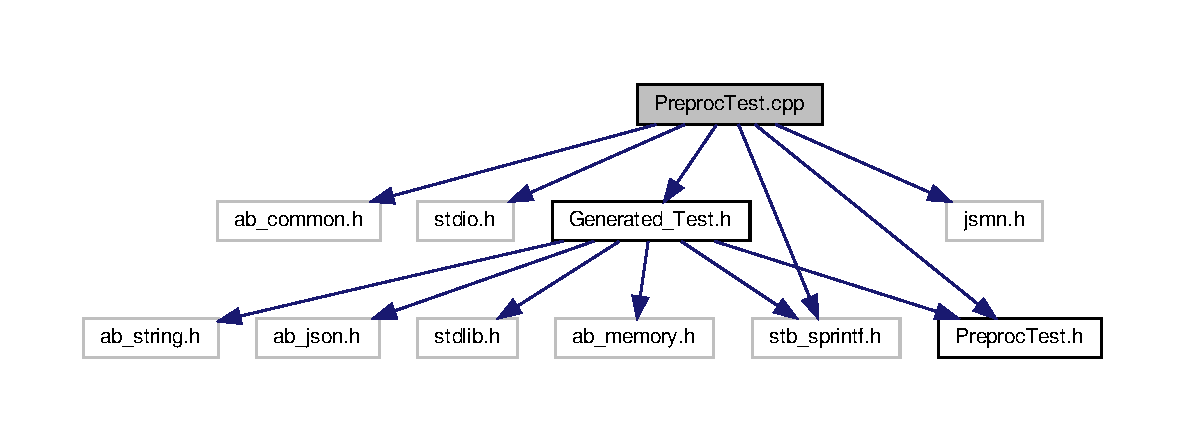
\includegraphics[width=350pt]{d7/d9c/PreprocTest_8cpp__incl}
\end{center}
\end{figure}
\doxysubsection*{Macros}
\begin{DoxyCompactItemize}
\item 
\#define \mbox{\hyperlink{PreprocTest_8cpp_a84802074473c7ddf6f95866d540f6e9a}{A\+B\+\_\+\+S\+T\+R\+I\+N\+G\+\_\+\+S\+RC}}
\item 
\#define \mbox{\hyperlink{PreprocTest_8cpp_a5a9e94a82063f4627c3af07f531c9bfc}{A\+B\+\_\+\+M\+E\+M\+O\+R\+Y\+\_\+\+S\+RC}}
\item 
\#define \mbox{\hyperlink{PreprocTest_8cpp_a72e86a5637e8283e65c1e3143948cf55}{A\+B\+\_\+\+J\+S\+O\+N\+\_\+\+S\+RC}}
\item 
\#define \mbox{\hyperlink{PreprocTest_8cpp_a400a089a07d326740f3e10fceec916c3}{G\+E\+N\+\_\+\+J\+S\+M\+N\+\_\+\+H\+E\+A\+D\+ER}}
\item 
\#define \mbox{\hyperlink{PreprocTest_8cpp_a82a16301fbc2b5f82923762b30a26b11}{G\+E\+N\+E\+R\+A\+T\+E\+D\+\_\+\+T\+E\+S\+T\+\_\+\+S\+RC}}
\item 
\#define \mbox{\hyperlink{PreprocTest_8cpp_aa3df03d3e4d8ee0f7f2c7ec39f4adb4b}{J\+S\+M\+N\+\_\+\+S\+RC}}
\item 
\#define \mbox{\hyperlink{PreprocTest_8cpp_a840dcc5088daf9a542cceb05e306855c}{S\+T\+B\+\_\+\+S\+P\+R\+I\+N\+T\+F\+\_\+\+I\+M\+P\+L\+E\+M\+E\+N\+T\+A\+T\+I\+ON}}
\end{DoxyCompactItemize}
\doxysubsection*{Functions}
\begin{DoxyCompactItemize}
\item 
\mbox{\hyperlink{PreprocTest_8cpp_a47061d27749d7e9de66e4e834ab28848}{S\+T\+A\+T\+E\+M\+A\+C\+H\+I\+NE}} (test\+\_\+statemachine, \mbox{\hyperlink{structtest__type}{test\+\_\+type}}, \mbox{\hyperlink{PreprocTest_8h_a55ed691059222a58555cf9992ec14431}{test\+\_\+cmd}}, int Int, char const $\ast$String)
\item 
\mbox{\hyperlink{PreprocTest_8cpp_ab6c57dcff4bca075ce03bbe119d0b4dd}{T\+E\+S\+T\+\_\+\+S\+T\+A\+T\+E\+M\+A\+C\+H\+I\+NE}} (Idle)
\begin{DoxyCompactList}\small\item\em Forward declaration for Idle(). \end{DoxyCompactList}\item 
\mbox{\hyperlink{PreprocTest_8cpp_aed31da543c10eab9ca01e8b7f1e299cd}{T\+E\+S\+T\+\_\+\+S\+T\+A\+T\+E\+M\+A\+C\+H\+I\+NE}} (Running)
\begin{DoxyCompactList}\small\item\em Forward declaration for Running(). \end{DoxyCompactList}\item 
void \mbox{\hyperlink{PreprocTest_8cpp_a211bd71013d900e07a4105d067d0d864}{Print\+Queue}} (\mbox{\hyperlink{structtest__cmd__queue}{test\+\_\+cmd\+\_\+queue}} $\ast$Queue)
\item 
int \mbox{\hyperlink{PreprocTest_8cpp_a0ddf1224851353fc92bfbff6f499fa97}{main}} (int argc, char $\ast$argv\mbox{[}$\,$\mbox{]})
\end{DoxyCompactItemize}


\doxysubsection{Macro Definition Documentation}
\mbox{\Hypertarget{PreprocTest_8cpp_a72e86a5637e8283e65c1e3143948cf55}\label{PreprocTest_8cpp_a72e86a5637e8283e65c1e3143948cf55}} 
\index{PreprocTest.cpp@{PreprocTest.cpp}!AB\_JSON\_SRC@{AB\_JSON\_SRC}}
\index{AB\_JSON\_SRC@{AB\_JSON\_SRC}!PreprocTest.cpp@{PreprocTest.cpp}}
\doxysubsubsection{\texorpdfstring{AB\_JSON\_SRC}{AB\_JSON\_SRC}}
{\footnotesize\ttfamily \#define A\+B\+\_\+\+J\+S\+O\+N\+\_\+\+S\+RC}

\mbox{\Hypertarget{PreprocTest_8cpp_a5a9e94a82063f4627c3af07f531c9bfc}\label{PreprocTest_8cpp_a5a9e94a82063f4627c3af07f531c9bfc}} 
\index{PreprocTest.cpp@{PreprocTest.cpp}!AB\_MEMORY\_SRC@{AB\_MEMORY\_SRC}}
\index{AB\_MEMORY\_SRC@{AB\_MEMORY\_SRC}!PreprocTest.cpp@{PreprocTest.cpp}}
\doxysubsubsection{\texorpdfstring{AB\_MEMORY\_SRC}{AB\_MEMORY\_SRC}}
{\footnotesize\ttfamily \#define A\+B\+\_\+\+M\+E\+M\+O\+R\+Y\+\_\+\+S\+RC}

\mbox{\Hypertarget{PreprocTest_8cpp_a84802074473c7ddf6f95866d540f6e9a}\label{PreprocTest_8cpp_a84802074473c7ddf6f95866d540f6e9a}} 
\index{PreprocTest.cpp@{PreprocTest.cpp}!AB\_STRING\_SRC@{AB\_STRING\_SRC}}
\index{AB\_STRING\_SRC@{AB\_STRING\_SRC}!PreprocTest.cpp@{PreprocTest.cpp}}
\doxysubsubsection{\texorpdfstring{AB\_STRING\_SRC}{AB\_STRING\_SRC}}
{\footnotesize\ttfamily \#define A\+B\+\_\+\+S\+T\+R\+I\+N\+G\+\_\+\+S\+RC}

\mbox{\Hypertarget{PreprocTest_8cpp_a400a089a07d326740f3e10fceec916c3}\label{PreprocTest_8cpp_a400a089a07d326740f3e10fceec916c3}} 
\index{PreprocTest.cpp@{PreprocTest.cpp}!GEN\_JSMN\_HEADER@{GEN\_JSMN\_HEADER}}
\index{GEN\_JSMN\_HEADER@{GEN\_JSMN\_HEADER}!PreprocTest.cpp@{PreprocTest.cpp}}
\doxysubsubsection{\texorpdfstring{GEN\_JSMN\_HEADER}{GEN\_JSMN\_HEADER}}
{\footnotesize\ttfamily \#define G\+E\+N\+\_\+\+J\+S\+M\+N\+\_\+\+H\+E\+A\+D\+ER}

\mbox{\Hypertarget{PreprocTest_8cpp_a82a16301fbc2b5f82923762b30a26b11}\label{PreprocTest_8cpp_a82a16301fbc2b5f82923762b30a26b11}} 
\index{PreprocTest.cpp@{PreprocTest.cpp}!GENERATED\_TEST\_SRC@{GENERATED\_TEST\_SRC}}
\index{GENERATED\_TEST\_SRC@{GENERATED\_TEST\_SRC}!PreprocTest.cpp@{PreprocTest.cpp}}
\doxysubsubsection{\texorpdfstring{GENERATED\_TEST\_SRC}{GENERATED\_TEST\_SRC}}
{\footnotesize\ttfamily \#define G\+E\+N\+E\+R\+A\+T\+E\+D\+\_\+\+T\+E\+S\+T\+\_\+\+S\+RC}

\mbox{\Hypertarget{PreprocTest_8cpp_aa3df03d3e4d8ee0f7f2c7ec39f4adb4b}\label{PreprocTest_8cpp_aa3df03d3e4d8ee0f7f2c7ec39f4adb4b}} 
\index{PreprocTest.cpp@{PreprocTest.cpp}!JSMN\_SRC@{JSMN\_SRC}}
\index{JSMN\_SRC@{JSMN\_SRC}!PreprocTest.cpp@{PreprocTest.cpp}}
\doxysubsubsection{\texorpdfstring{JSMN\_SRC}{JSMN\_SRC}}
{\footnotesize\ttfamily \#define J\+S\+M\+N\+\_\+\+S\+RC}

\mbox{\Hypertarget{PreprocTest_8cpp_a840dcc5088daf9a542cceb05e306855c}\label{PreprocTest_8cpp_a840dcc5088daf9a542cceb05e306855c}} 
\index{PreprocTest.cpp@{PreprocTest.cpp}!STB\_SPRINTF\_IMPLEMENTATION@{STB\_SPRINTF\_IMPLEMENTATION}}
\index{STB\_SPRINTF\_IMPLEMENTATION@{STB\_SPRINTF\_IMPLEMENTATION}!PreprocTest.cpp@{PreprocTest.cpp}}
\doxysubsubsection{\texorpdfstring{STB\_SPRINTF\_IMPLEMENTATION}{STB\_SPRINTF\_IMPLEMENTATION}}
{\footnotesize\ttfamily \#define S\+T\+B\+\_\+\+S\+P\+R\+I\+N\+T\+F\+\_\+\+I\+M\+P\+L\+E\+M\+E\+N\+T\+A\+T\+I\+ON}



\doxysubsection{Function Documentation}
\mbox{\Hypertarget{PreprocTest_8cpp_a0ddf1224851353fc92bfbff6f499fa97}\label{PreprocTest_8cpp_a0ddf1224851353fc92bfbff6f499fa97}} 
\index{PreprocTest.cpp@{PreprocTest.cpp}!main@{main}}
\index{main@{main}!PreprocTest.cpp@{PreprocTest.cpp}}
\doxysubsubsection{\texorpdfstring{main()}{main()}}
{\footnotesize\ttfamily int main (\begin{DoxyParamCaption}\item[{int}]{argc,  }\item[{char $\ast$}]{argv\mbox{[}$\,$\mbox{]} }\end{DoxyParamCaption})}

\mbox{\Hypertarget{PreprocTest_8cpp_a211bd71013d900e07a4105d067d0d864}\label{PreprocTest_8cpp_a211bd71013d900e07a4105d067d0d864}} 
\index{PreprocTest.cpp@{PreprocTest.cpp}!PrintQueue@{PrintQueue}}
\index{PrintQueue@{PrintQueue}!PreprocTest.cpp@{PreprocTest.cpp}}
\doxysubsubsection{\texorpdfstring{PrintQueue()}{PrintQueue()}}
{\footnotesize\ttfamily void Print\+Queue (\begin{DoxyParamCaption}\item[{\mbox{\hyperlink{structtest__cmd__queue}{test\+\_\+cmd\+\_\+queue}} $\ast$}]{Queue }\end{DoxyParamCaption})}

\mbox{\Hypertarget{PreprocTest_8cpp_a47061d27749d7e9de66e4e834ab28848}\label{PreprocTest_8cpp_a47061d27749d7e9de66e4e834ab28848}} 
\index{PreprocTest.cpp@{PreprocTest.cpp}!STATEMACHINE@{STATEMACHINE}}
\index{STATEMACHINE@{STATEMACHINE}!PreprocTest.cpp@{PreprocTest.cpp}}
\doxysubsubsection{\texorpdfstring{STATEMACHINE()}{STATEMACHINE()}}
{\footnotesize\ttfamily S\+T\+A\+T\+E\+M\+A\+C\+H\+I\+NE (\begin{DoxyParamCaption}\item[{test\+\_\+statemachine}]{,  }\item[{\mbox{\hyperlink{structtest__type}{test\+\_\+type}}}]{,  }\item[{\mbox{\hyperlink{PreprocTest_8h_a55ed691059222a58555cf9992ec14431}{test\+\_\+cmd}}}]{,  }\item[{int}]{Int,  }\item[{char const $\ast$}]{String }\end{DoxyParamCaption})}

\mbox{\Hypertarget{PreprocTest_8cpp_ab6c57dcff4bca075ce03bbe119d0b4dd}\label{PreprocTest_8cpp_ab6c57dcff4bca075ce03bbe119d0b4dd}} 
\index{PreprocTest.cpp@{PreprocTest.cpp}!TEST\_STATEMACHINE@{TEST\_STATEMACHINE}}
\index{TEST\_STATEMACHINE@{TEST\_STATEMACHINE}!PreprocTest.cpp@{PreprocTest.cpp}}
\doxysubsubsection{\texorpdfstring{TEST\_STATEMACHINE()}{TEST\_STATEMACHINE()}\hspace{0.1cm}{\footnotesize\ttfamily [1/2]}}
{\footnotesize\ttfamily T\+E\+S\+T\+\_\+\+S\+T\+A\+T\+E\+M\+A\+C\+H\+I\+NE (\begin{DoxyParamCaption}\item[{Idle}]{ }\end{DoxyParamCaption})}



Forward declaration for Idle(). 

\mbox{\Hypertarget{PreprocTest_8cpp_aed31da543c10eab9ca01e8b7f1e299cd}\label{PreprocTest_8cpp_aed31da543c10eab9ca01e8b7f1e299cd}} 
\index{PreprocTest.cpp@{PreprocTest.cpp}!TEST\_STATEMACHINE@{TEST\_STATEMACHINE}}
\index{TEST\_STATEMACHINE@{TEST\_STATEMACHINE}!PreprocTest.cpp@{PreprocTest.cpp}}
\doxysubsubsection{\texorpdfstring{TEST\_STATEMACHINE()}{TEST\_STATEMACHINE()}\hspace{0.1cm}{\footnotesize\ttfamily [2/2]}}
{\footnotesize\ttfamily T\+E\+S\+T\+\_\+\+S\+T\+A\+T\+E\+M\+A\+C\+H\+I\+NE (\begin{DoxyParamCaption}\item[{Running}]{ }\end{DoxyParamCaption})}



Forward declaration for Running(). 


\hypertarget{PreprocTest_8h}{}\doxysection{Preproc\+Test.\+h File Reference}
\label{PreprocTest_8h}\index{PreprocTest.h@{PreprocTest.h}}
This graph shows which files directly or indirectly include this file\+:
\nopagebreak
\begin{figure}[H]
\begin{center}
\leavevmode
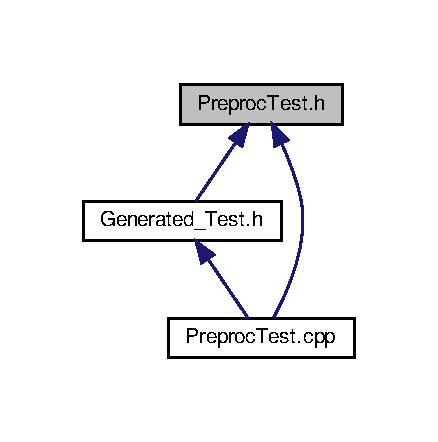
\includegraphics[width=330pt]{dc/dd7/PreprocTest_8h__dep__incl}
\end{center}
\end{figure}
\doxysubsection*{Classes}
\begin{DoxyCompactItemize}
\item 
struct \mbox{\hyperlink{structtest__type}{test\+\_\+type}}
\item 
struct \mbox{\hyperlink{structmy__json__test}{my\+\_\+json\+\_\+test}}
\end{DoxyCompactItemize}
\doxysubsection*{Enumerations}
\begin{DoxyCompactItemize}
\item 
enum \mbox{\hyperlink{PreprocTest_8h_a55ed691059222a58555cf9992ec14431}{test\+\_\+cmd}} \{ \newline
\mbox{\hyperlink{PreprocTest_8h_a55ed691059222a58555cf9992ec14431a1a004f5abe2b334db21328be1ea6b593}{test\+\_\+cmd\+::\+N\+OP}}, 
\mbox{\hyperlink{PreprocTest_8h_a55ed691059222a58555cf9992ec14431a1ed25d14e3a228b0089b334bdbca5769}{test\+\_\+cmd\+::\+Command1}}, 
\mbox{\hyperlink{PreprocTest_8h_a55ed691059222a58555cf9992ec14431a0c33f49f722805e5a6f6f759b491fa2a}{test\+\_\+cmd\+::\+Command2}}, 
\mbox{\hyperlink{PreprocTest_8h_a55ed691059222a58555cf9992ec14431a732a6c81e81f68d48d63e795bd06ab22}{test\+\_\+cmd\+::\+Command3}}, 
\newline
\mbox{\hyperlink{PreprocTest_8h_a55ed691059222a58555cf9992ec14431aeb4001380fa7b2b0c963a882c2305280}{test\+\_\+cmd\+::\+Command4}}, 
\mbox{\hyperlink{PreprocTest_8h_a55ed691059222a58555cf9992ec14431ad55b30607c2a9a2616347d6edb789f6b}{test\+\_\+cmd\+::\+Last}}
 \}
\item 
enum \mbox{\hyperlink{PreprocTest_8h_a081cf1a0e70d6e2bd48c98f457742877}{en\+Colours}} \{ \mbox{\hyperlink{PreprocTest_8h_a081cf1a0e70d6e2bd48c98f457742877aee38e4d5dd68c4e440825018d549cb47}{en\+Colours\+::\+Red}}, 
\mbox{\hyperlink{PreprocTest_8h_a081cf1a0e70d6e2bd48c98f457742877ad382816a3cbeed082c9e216e7392eed1}{en\+Colours\+::\+Green}}, 
\mbox{\hyperlink{PreprocTest_8h_a081cf1a0e70d6e2bd48c98f457742877a9594eec95be70e7b1710f730fdda33d9}{en\+Colours\+::\+Blue}}
 \}
\end{DoxyCompactItemize}
\doxysubsection*{Functions}
\begin{DoxyCompactItemize}
\item 
\mbox{\hyperlink{PreprocTest_8h_a2606cd56d2d8f567785bde5848176722}{T\+AG}} (J\+S\+ON, Strings, Label\+:\+Object)
\end{DoxyCompactItemize}


\doxysubsection{Enumeration Type Documentation}
\mbox{\Hypertarget{PreprocTest_8h_a081cf1a0e70d6e2bd48c98f457742877}\label{PreprocTest_8h_a081cf1a0e70d6e2bd48c98f457742877}} 
\index{PreprocTest.h@{PreprocTest.h}!enColours@{enColours}}
\index{enColours@{enColours}!PreprocTest.h@{PreprocTest.h}}
\doxysubsubsection{\texorpdfstring{enColours}{enColours}}
{\footnotesize\ttfamily enum \mbox{\hyperlink{PreprocTest_8h_a081cf1a0e70d6e2bd48c98f457742877}{en\+Colours}}\hspace{0.3cm}{\ttfamily [strong]}}

\begin{DoxyEnumFields}{Enumerator}
\raisebox{\heightof{T}}[0pt][0pt]{\index{Red@{Red}!PreprocTest.h@{PreprocTest.h}}\index{PreprocTest.h@{PreprocTest.h}!Red@{Red}}}\mbox{\Hypertarget{PreprocTest_8h_a081cf1a0e70d6e2bd48c98f457742877aee38e4d5dd68c4e440825018d549cb47}\label{PreprocTest_8h_a081cf1a0e70d6e2bd48c98f457742877aee38e4d5dd68c4e440825018d549cb47}} 
Red&\\
\hline

\raisebox{\heightof{T}}[0pt][0pt]{\index{Green@{Green}!PreprocTest.h@{PreprocTest.h}}\index{PreprocTest.h@{PreprocTest.h}!Green@{Green}}}\mbox{\Hypertarget{PreprocTest_8h_a081cf1a0e70d6e2bd48c98f457742877ad382816a3cbeed082c9e216e7392eed1}\label{PreprocTest_8h_a081cf1a0e70d6e2bd48c98f457742877ad382816a3cbeed082c9e216e7392eed1}} 
Green&\\
\hline

\raisebox{\heightof{T}}[0pt][0pt]{\index{Blue@{Blue}!PreprocTest.h@{PreprocTest.h}}\index{PreprocTest.h@{PreprocTest.h}!Blue@{Blue}}}\mbox{\Hypertarget{PreprocTest_8h_a081cf1a0e70d6e2bd48c98f457742877a9594eec95be70e7b1710f730fdda33d9}\label{PreprocTest_8h_a081cf1a0e70d6e2bd48c98f457742877a9594eec95be70e7b1710f730fdda33d9}} 
Blue&\\
\hline

\end{DoxyEnumFields}
\mbox{\Hypertarget{PreprocTest_8h_a55ed691059222a58555cf9992ec14431}\label{PreprocTest_8h_a55ed691059222a58555cf9992ec14431}} 
\index{PreprocTest.h@{PreprocTest.h}!test\_cmd@{test\_cmd}}
\index{test\_cmd@{test\_cmd}!PreprocTest.h@{PreprocTest.h}}
\doxysubsubsection{\texorpdfstring{test\_cmd}{test\_cmd}}
{\footnotesize\ttfamily enum \mbox{\hyperlink{PreprocTest_8h_a55ed691059222a58555cf9992ec14431}{test\+\_\+cmd}}\hspace{0.3cm}{\ttfamily [strong]}}

\begin{DoxyEnumFields}{Enumerator}
\raisebox{\heightof{T}}[0pt][0pt]{\index{NOP@{NOP}!PreprocTest.h@{PreprocTest.h}}\index{PreprocTest.h@{PreprocTest.h}!NOP@{NOP}}}\mbox{\Hypertarget{PreprocTest_8h_a55ed691059222a58555cf9992ec14431a1a004f5abe2b334db21328be1ea6b593}\label{PreprocTest_8h_a55ed691059222a58555cf9992ec14431a1a004f5abe2b334db21328be1ea6b593}} 
N\+OP&\\
\hline

\raisebox{\heightof{T}}[0pt][0pt]{\index{Command1@{Command1}!PreprocTest.h@{PreprocTest.h}}\index{PreprocTest.h@{PreprocTest.h}!Command1@{Command1}}}\mbox{\Hypertarget{PreprocTest_8h_a55ed691059222a58555cf9992ec14431a1ed25d14e3a228b0089b334bdbca5769}\label{PreprocTest_8h_a55ed691059222a58555cf9992ec14431a1ed25d14e3a228b0089b334bdbca5769}} 
Command1&\\
\hline

\raisebox{\heightof{T}}[0pt][0pt]{\index{Command2@{Command2}!PreprocTest.h@{PreprocTest.h}}\index{PreprocTest.h@{PreprocTest.h}!Command2@{Command2}}}\mbox{\Hypertarget{PreprocTest_8h_a55ed691059222a58555cf9992ec14431a0c33f49f722805e5a6f6f759b491fa2a}\label{PreprocTest_8h_a55ed691059222a58555cf9992ec14431a0c33f49f722805e5a6f6f759b491fa2a}} 
Command2&\\
\hline

\raisebox{\heightof{T}}[0pt][0pt]{\index{Command3@{Command3}!PreprocTest.h@{PreprocTest.h}}\index{PreprocTest.h@{PreprocTest.h}!Command3@{Command3}}}\mbox{\Hypertarget{PreprocTest_8h_a55ed691059222a58555cf9992ec14431a732a6c81e81f68d48d63e795bd06ab22}\label{PreprocTest_8h_a55ed691059222a58555cf9992ec14431a732a6c81e81f68d48d63e795bd06ab22}} 
Command3&\\
\hline

\raisebox{\heightof{T}}[0pt][0pt]{\index{Command4@{Command4}!PreprocTest.h@{PreprocTest.h}}\index{PreprocTest.h@{PreprocTest.h}!Command4@{Command4}}}\mbox{\Hypertarget{PreprocTest_8h_a55ed691059222a58555cf9992ec14431aeb4001380fa7b2b0c963a882c2305280}\label{PreprocTest_8h_a55ed691059222a58555cf9992ec14431aeb4001380fa7b2b0c963a882c2305280}} 
Command4&\\
\hline

\raisebox{\heightof{T}}[0pt][0pt]{\index{Last@{Last}!PreprocTest.h@{PreprocTest.h}}\index{PreprocTest.h@{PreprocTest.h}!Last@{Last}}}\mbox{\Hypertarget{PreprocTest_8h_a55ed691059222a58555cf9992ec14431ad55b30607c2a9a2616347d6edb789f6b}\label{PreprocTest_8h_a55ed691059222a58555cf9992ec14431ad55b30607c2a9a2616347d6edb789f6b}} 
Last&\\
\hline

\end{DoxyEnumFields}


\doxysubsection{Function Documentation}
\mbox{\Hypertarget{PreprocTest_8h_a2606cd56d2d8f567785bde5848176722}\label{PreprocTest_8h_a2606cd56d2d8f567785bde5848176722}} 
\index{PreprocTest.h@{PreprocTest.h}!TAG@{TAG}}
\index{TAG@{TAG}!PreprocTest.h@{PreprocTest.h}}
\doxysubsubsection{\texorpdfstring{TAG()}{TAG()}}
{\footnotesize\ttfamily T\+AG (\begin{DoxyParamCaption}\item[{J\+S\+ON}]{,  }\item[{Strings}]{,  }\item[{Label\+:\+Object}]{ }\end{DoxyParamCaption})}


\hypertarget{Readme_8md}{}\doxysection{Readme.\+md File Reference}
\label{Readme_8md}\index{Readme.md@{Readme.md}}

\hypertarget{test__preprocessor_8cpp}{}\section{test\+\_\+preprocessor.\+cpp File Reference}
\label{test__preprocessor_8cpp}\index{test\+\_\+preprocessor.\+cpp@{test\+\_\+preprocessor.\+cpp}}
{\ttfamily \#include \char`\"{}mwp\+\_\+302-\/preprocessor.\+h\char`\"{}}\newline
{\ttfamily \#include $<$string.\+h$>$}\newline
Include dependency graph for test\+\_\+preprocessor.\+cpp\+:
\nopagebreak
\begin{figure}[H]
\begin{center}
\leavevmode
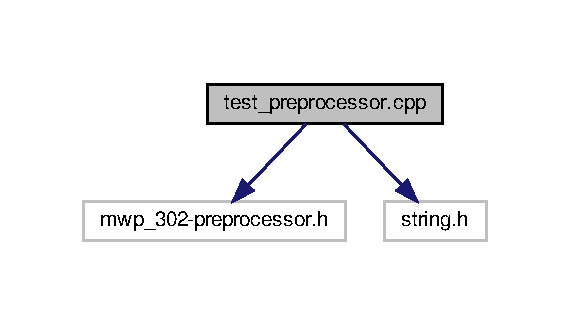
\includegraphics[width=274pt]{d0/dca/test__preprocessor_8cpp__incl}
\end{center}
\end{figure}
\subsection*{Classes}
\begin{DoxyCompactItemize}
\item 
struct \hyperlink{structtest__token__list__item}{test\+\_\+token\+\_\+list\+\_\+item}
\item 
struct \hyperlink{structtest__suite__token__list__item}{test\+\_\+suite\+\_\+token\+\_\+list\+\_\+item}
\item 
struct \hyperlink{structdata}{data}
\end{DoxyCompactItemize}
\subsection*{Functions}
\begin{DoxyCompactItemize}
\item 
void \hyperlink{test__preprocessor_8cpp_a8cf6633d3d75aceae72ac20116f1ea64}{Parse\+Test\+Function\+Name} (tokenizer $\ast$Tokenizer, memory\+\_\+arena $\ast$Memory, \hyperlink{structtest__token__list__item}{test\+\_\+token\+\_\+list\+\_\+item} $\ast$Tests\+Head)
\begin{DoxyCompactList}\small\item\em Parsing Functions. \end{DoxyCompactList}\item 
b8 \hyperlink{test__preprocessor_8cpp_a520eb11766981c66222227c38ec5dd64}{Parse\+Suite\+List} (tokenizer $\ast$Tokenizer, \hyperlink{structdata}{data} $\ast$Data, \hyperlink{structtest__suite__token__list__item}{test\+\_\+suite\+\_\+token\+\_\+list\+\_\+item} $\ast$$\ast$Current\+Suite\+Out)
\item 
void \hyperlink{test__preprocessor_8cpp_a1c60a3447e242ae37be6dd67dea3c2ad}{Parse\+Steps\+In\+Function} (tokenizer $\ast$Tokenizer, memory\+\_\+arena $\ast$Memory, token\+\_\+list\+\_\+item $\ast$Steps\+Head)
\item 
b8 \hyperlink{test__preprocessor_8cpp_afc4b46bb2585cb0823527d2f2d9b2ef1}{Parse\+Test\+Function} (tokenizer $\ast$Tokenizer, memory\+\_\+arena $\ast$Memory, \hyperlink{structtest__suite__token__list__item}{test\+\_\+suite\+\_\+token\+\_\+list\+\_\+item} $\ast$Current\+Suite)
\item 
b8 \hyperlink{test__preprocessor_8cpp_af44fc9931e29323dd32b922f8ebce6f6}{Get\+Token\+From\+Define} (tokenizer $\ast$Tokenizer, \hyperlink{structtoken}{token} $\ast$Function\+Name\+Out)
\item 
b8 \hyperlink{test__preprocessor_8cpp_a03c849c4aa8eac0edbed867344b6d7fd}{Parse\+Test\+Suite\+Init\+Function} (tokenizer $\ast$Tokenizer, memory\+\_\+arena $\ast$Memory, \hyperlink{structtest__suite__token__list__item}{test\+\_\+suite\+\_\+token\+\_\+list\+\_\+item} $\ast$Current\+Suite)
\item 
b8 \hyperlink{test__preprocessor_8cpp_ad8f61a6c142f245e827c7b22cd180764}{Parse\+Test\+Suite\+Shutdown\+Function} (tokenizer $\ast$Tokenizer, memory\+\_\+arena $\ast$Memory, \hyperlink{structtest__suite__token__list__item}{test\+\_\+suite\+\_\+token\+\_\+list\+\_\+item} $\ast$Current\+Suite)
\item 
int \hyperlink{test__preprocessor_8cpp_a3c04138a5bfe5d72780bb7e82a18e627}{main} (int argc, char $\ast$$\ast$argv)
\end{DoxyCompactItemize}


\subsection{Function Documentation}
\mbox{\Hypertarget{test__preprocessor_8cpp_af44fc9931e29323dd32b922f8ebce6f6}\label{test__preprocessor_8cpp_af44fc9931e29323dd32b922f8ebce6f6}} 
\index{test\+\_\+preprocessor.\+cpp@{test\+\_\+preprocessor.\+cpp}!Get\+Token\+From\+Define@{Get\+Token\+From\+Define}}
\index{Get\+Token\+From\+Define@{Get\+Token\+From\+Define}!test\+\_\+preprocessor.\+cpp@{test\+\_\+preprocessor.\+cpp}}
\subsubsection{\texorpdfstring{Get\+Token\+From\+Define()}{GetTokenFromDefine()}}
{\footnotesize\ttfamily b8 Get\+Token\+From\+Define (\begin{DoxyParamCaption}\item[{tokenizer $\ast$}]{Tokenizer,  }\item[{\hyperlink{structtoken}{token} $\ast$}]{Function\+Name\+Out }\end{DoxyParamCaption})}

\mbox{\Hypertarget{test__preprocessor_8cpp_a3c04138a5bfe5d72780bb7e82a18e627}\label{test__preprocessor_8cpp_a3c04138a5bfe5d72780bb7e82a18e627}} 
\index{test\+\_\+preprocessor.\+cpp@{test\+\_\+preprocessor.\+cpp}!main@{main}}
\index{main@{main}!test\+\_\+preprocessor.\+cpp@{test\+\_\+preprocessor.\+cpp}}
\subsubsection{\texorpdfstring{main()}{main()}}
{\footnotesize\ttfamily int main (\begin{DoxyParamCaption}\item[{int}]{argc,  }\item[{char $\ast$$\ast$}]{argv }\end{DoxyParamCaption})}

\mbox{\Hypertarget{test__preprocessor_8cpp_a1c60a3447e242ae37be6dd67dea3c2ad}\label{test__preprocessor_8cpp_a1c60a3447e242ae37be6dd67dea3c2ad}} 
\index{test\+\_\+preprocessor.\+cpp@{test\+\_\+preprocessor.\+cpp}!Parse\+Steps\+In\+Function@{Parse\+Steps\+In\+Function}}
\index{Parse\+Steps\+In\+Function@{Parse\+Steps\+In\+Function}!test\+\_\+preprocessor.\+cpp@{test\+\_\+preprocessor.\+cpp}}
\subsubsection{\texorpdfstring{Parse\+Steps\+In\+Function()}{ParseStepsInFunction()}}
{\footnotesize\ttfamily void Parse\+Steps\+In\+Function (\begin{DoxyParamCaption}\item[{tokenizer $\ast$}]{Tokenizer,  }\item[{memory\+\_\+arena $\ast$}]{Memory,  }\item[{token\+\_\+list\+\_\+item $\ast$}]{Steps\+Head }\end{DoxyParamCaption})}

\mbox{\Hypertarget{test__preprocessor_8cpp_a520eb11766981c66222227c38ec5dd64}\label{test__preprocessor_8cpp_a520eb11766981c66222227c38ec5dd64}} 
\index{test\+\_\+preprocessor.\+cpp@{test\+\_\+preprocessor.\+cpp}!Parse\+Suite\+List@{Parse\+Suite\+List}}
\index{Parse\+Suite\+List@{Parse\+Suite\+List}!test\+\_\+preprocessor.\+cpp@{test\+\_\+preprocessor.\+cpp}}
\subsubsection{\texorpdfstring{Parse\+Suite\+List()}{ParseSuiteList()}}
{\footnotesize\ttfamily b8 Parse\+Suite\+List (\begin{DoxyParamCaption}\item[{tokenizer $\ast$}]{Tokenizer,  }\item[{\hyperlink{structdata}{data} $\ast$}]{Data,  }\item[{\hyperlink{structtest__suite__token__list__item}{test\+\_\+suite\+\_\+token\+\_\+list\+\_\+item} $\ast$$\ast$}]{Current\+Suite\+Out }\end{DoxyParamCaption})}

\mbox{\Hypertarget{test__preprocessor_8cpp_afc4b46bb2585cb0823527d2f2d9b2ef1}\label{test__preprocessor_8cpp_afc4b46bb2585cb0823527d2f2d9b2ef1}} 
\index{test\+\_\+preprocessor.\+cpp@{test\+\_\+preprocessor.\+cpp}!Parse\+Test\+Function@{Parse\+Test\+Function}}
\index{Parse\+Test\+Function@{Parse\+Test\+Function}!test\+\_\+preprocessor.\+cpp@{test\+\_\+preprocessor.\+cpp}}
\subsubsection{\texorpdfstring{Parse\+Test\+Function()}{ParseTestFunction()}}
{\footnotesize\ttfamily b8 Parse\+Test\+Function (\begin{DoxyParamCaption}\item[{tokenizer $\ast$}]{Tokenizer,  }\item[{memory\+\_\+arena $\ast$}]{Memory,  }\item[{\hyperlink{structtest__suite__token__list__item}{test\+\_\+suite\+\_\+token\+\_\+list\+\_\+item} $\ast$}]{Current\+Suite }\end{DoxyParamCaption})}

\mbox{\Hypertarget{test__preprocessor_8cpp_a8cf6633d3d75aceae72ac20116f1ea64}\label{test__preprocessor_8cpp_a8cf6633d3d75aceae72ac20116f1ea64}} 
\index{test\+\_\+preprocessor.\+cpp@{test\+\_\+preprocessor.\+cpp}!Parse\+Test\+Function\+Name@{Parse\+Test\+Function\+Name}}
\index{Parse\+Test\+Function\+Name@{Parse\+Test\+Function\+Name}!test\+\_\+preprocessor.\+cpp@{test\+\_\+preprocessor.\+cpp}}
\subsubsection{\texorpdfstring{Parse\+Test\+Function\+Name()}{ParseTestFunctionName()}}
{\footnotesize\ttfamily void Parse\+Test\+Function\+Name (\begin{DoxyParamCaption}\item[{tokenizer $\ast$}]{Tokenizer,  }\item[{memory\+\_\+arena $\ast$}]{Memory,  }\item[{\hyperlink{structtest__token__list__item}{test\+\_\+token\+\_\+list\+\_\+item} $\ast$}]{Tests\+Head }\end{DoxyParamCaption})}



Parsing Functions. 

\mbox{\Hypertarget{test__preprocessor_8cpp_a03c849c4aa8eac0edbed867344b6d7fd}\label{test__preprocessor_8cpp_a03c849c4aa8eac0edbed867344b6d7fd}} 
\index{test\+\_\+preprocessor.\+cpp@{test\+\_\+preprocessor.\+cpp}!Parse\+Test\+Suite\+Init\+Function@{Parse\+Test\+Suite\+Init\+Function}}
\index{Parse\+Test\+Suite\+Init\+Function@{Parse\+Test\+Suite\+Init\+Function}!test\+\_\+preprocessor.\+cpp@{test\+\_\+preprocessor.\+cpp}}
\subsubsection{\texorpdfstring{Parse\+Test\+Suite\+Init\+Function()}{ParseTestSuiteInitFunction()}}
{\footnotesize\ttfamily b8 Parse\+Test\+Suite\+Init\+Function (\begin{DoxyParamCaption}\item[{tokenizer $\ast$}]{Tokenizer,  }\item[{memory\+\_\+arena $\ast$}]{Memory,  }\item[{\hyperlink{structtest__suite__token__list__item}{test\+\_\+suite\+\_\+token\+\_\+list\+\_\+item} $\ast$}]{Current\+Suite }\end{DoxyParamCaption})}

\mbox{\Hypertarget{test__preprocessor_8cpp_ad8f61a6c142f245e827c7b22cd180764}\label{test__preprocessor_8cpp_ad8f61a6c142f245e827c7b22cd180764}} 
\index{test\+\_\+preprocessor.\+cpp@{test\+\_\+preprocessor.\+cpp}!Parse\+Test\+Suite\+Shutdown\+Function@{Parse\+Test\+Suite\+Shutdown\+Function}}
\index{Parse\+Test\+Suite\+Shutdown\+Function@{Parse\+Test\+Suite\+Shutdown\+Function}!test\+\_\+preprocessor.\+cpp@{test\+\_\+preprocessor.\+cpp}}
\subsubsection{\texorpdfstring{Parse\+Test\+Suite\+Shutdown\+Function()}{ParseTestSuiteShutdownFunction()}}
{\footnotesize\ttfamily b8 Parse\+Test\+Suite\+Shutdown\+Function (\begin{DoxyParamCaption}\item[{tokenizer $\ast$}]{Tokenizer,  }\item[{memory\+\_\+arena $\ast$}]{Memory,  }\item[{\hyperlink{structtest__suite__token__list__item}{test\+\_\+suite\+\_\+token\+\_\+list\+\_\+item} $\ast$}]{Current\+Suite }\end{DoxyParamCaption})}


%--- End generated contents ---

% Index
\backmatter
\newpage
\phantomsection
\clearemptydoublepage
\addcontentsline{toc}{chapter}{Index}
\printindex

\end{document}
